%-----------
% thesis.tex
%-----------
% This is a template which hopefully is useful to anyone putting together their
% thesis.  It is usually a good idea to have one main file (such as this) which
% includes all your chapters.  That way you can work on separate chapters
% without having to compile your whole thesis.  I would also recommend not
% calling your files chap1.tex, chap2.tex etc., since you are bound to want to
% change the order around, and then the numberings will just cause confusion!
% My thesis can be downloaded from my website to see how this template could be
% used (http://www.staff.ncl.ac.uk/a.j.youd/), or you can e-mail me
% (anthony.youd@newcastle.ac.uk).  Questions/comments to this address as well.
%------------------------------------------------------------------------------

%------------------------------------------------------------------------------
% Set the class and font size.  The article class does not allow chapters, so
% you'll want to avoid that.  I used 11pt for final submission.
\documentclass[11pt,openright]{report}
%------------------------------------------------------------------------------

%------------------------------------------------------------------------------
% Set the left and right margins.  Remember, you will need to leave more space
% on the left, to allow for binding, when it comes to submission.  You can
% easily change the margins as you like, but I think there must be at least a
% 30mm margin on the binding edge.
%
% One-sided.
\usepackage[a4paper,left=35mm,right=25mm,top=40mm,bottom=35mm]{geometry}
%
% Two-sided.
%\usepackage[a4paper,twoside,left=35mm,right=25mm,top=40mm,bottom=35mm]{geometry}
%
% Centred.
%\usepackage[a4paper,left=30mm,right=30mm,top=40mm,bottom=35mm]{geometry}
%little 
%\usepackage[papersize={6in,9in},twoside,left=0.75in,right=0.5in,top=0.5in,bottom=0.5in,includehead, includefoot]{geometry}
%------------------------------------------------------------------------------

%------------------------------------------------------------------------------
% Uncomment the two lines below if you would prefer blank lines for paragraph
% breaks, rather than indents.
%\setlength{\parindent}{0em}
%\setlength{\parskip}{1ex}
%------------------------------------------------------------------------------

%------------------------------------------------------------------------------
% This line prevents LaTeX complaining about \headheight being too small.
\setlength{\headheight}{15pt}
%------------------------------------------------------------------------------

%------------------------------------------------------------------------------
% If you only want to include certain chapters in the final output, do
% something like the commented line below.  Note that the entire document must
% have been compiled at least once for references to work correctly.
%\includeonly{./conclusions/chapter}
%------------------------------------------------------------------------------

% The masthesis style file itself.  Many additional packages are already
% defined in the style file (inputs/masthesis.sty).  Either add your own
% packages there, or below the following line.
\usepackage{masthesis}

%blank page before chapter start
\makeatletter
\def\cleardoublepage{\clearpage\if@twoside \ifodd\c@page\else
\hbox{}
\vspace*{\fill}
\vspace{\fill}
\thispagestyle{empty}
\newpage
\if@twocolumn\hbox{}\newpage\fi\fi\fi}
\makeatother

% One-and-a-half or double-line spacing.  I used 1.5 for final submission.
\onehalfspacing
%\doublespacing

%\makeindex

\begin{document}
  \pagenumbering{roman}
  \phdtitle{A Numerical Study of Vortices and Turbulence in Quantum Fluids} % Title.
           {George William Stagg}       % Author.
           {fig/logo}                 % Graphic for the title page.
           {June $2016$}                % Date.

  \thispagestyle{empty}
  \cleardoublepage
  \begin{acknowledgements}
 I would like to thank \ldots [TO BE ADDED]
\end{acknowledgements}
\thispagestyle{empty}
                   % Acknowledgements.
  \newpage
  \begin{abstract}
An intriguing feature of quantum fluids is lack of excitations when the fluid velocity is slower than a critical value; above this velocity the flow becomes dissipative and, due to a direct consequence of quantum mechanical effects, macroscopic excitations are created in the form of quantised vortices with fixed circulation $\kappa$, proportional to Planck's constant. Quantum fluids also exhibit superfluidity; flow with the absence of viscosity. Recent experimental, numerical and theoretical studies have highlighted unexpected and remarkable similarities between turbulence in quantum fluids (consisting of the motion of many quantised vortices) and turbulence in ordinary classical fluids, despite the lack of viscosity and constrained vorticity.

In this thesis we quantitatively and qualitatively study the dynamics of these phenomena, from the production of a single vortex pair to the complex and chaotic motion of turbulent vortex tangles, in both superfluid Helium II and atomic Bose-Einstein condensates. We model the quantum fluids both at zero temperature and beyond through use of the Gross-Pitaevskii equation and its variants, in both two and three dimensions. Extensive numerical simulation of the Gross-Pitaevskii equation is performed, providing insight into the dynamics of quantum fluids in the presence of quantum turbulence.

We study the wake that forms behind various obstacle shapes in the presence of a superfluid flow, modelling ultra low temperature atomic BEC experiments.

We study the decay of quantum turbulence, generated by a large obstacle in an atomic BEC.

We consider a Bose gas at finite-temperature, and discuss how the thermal component affect vortex nucleation. 

Finally we study the effect of rough surfaces on superfluid flow, modelling the vibrating wire experiments in Helium II.


\end{abstract}
\thispagestyle{empty}
\cleardoublepage
                      % Abstract.
  \clearpage
  \thispagestyle{empty}
  \cleardoublepage
  \microtypesetup{protrusion=false}
  \tableofcontents

  %\listoffigures

  %\listoftables
  \microtypesetup{protrusion=true}

  \clearpage                            % End the current page making sure all
  \thispagestyle{empty}                 % tables/figures are printed.
  \cleardoublepage                      % Necessary for correct page numbering.

  \pagenumbering{arabic}                % Reset the page numbering style.

  \part{Introduction and Theory}
  \begin{chapter}{\label{cha:bose_gases}Introduction}
In quantum mechanics there are two classes of particle: bosons and fermions. Fermionic particles (such as electrons) follow Fermi-Dirac statistics, have half-integer spin, and obey the Pauli exclusion principle. Bosonic particles (such as photons) have integer spin, follow Bose-Einstein statistics and, unlike fermions, any number are permitted to occupy the same quantum state. In certain conditions, this latter property allows a large fraction of bosons to occupy the ground state macroscopically, a phenomenon known as Bose-Einstein condensation (BEC) \cite{Pethick,stringari}. Bose-Einstein condensation is as diverse as it is astonishing, appearing in all manner of physics from atomic physics to condensed matter to astrophysics, manifesting as unexpected phenomena such as superfluidity, quantised circulation and superconductivity \cite{griffin1996bose,tilley1990superfluidity}. These effects derive directly from quantum mechanics, and so the fluids that exhibit them are known as ``quantum fluids''.

\section{Bose-Einstein condensation}\label{section:becinintro}
The roots of the original prediction of Bose-Einstein condensation lies with Indian scientist, Satyendra Nath Bose. In 1924 Bose re-derived Planck's law of black-body radiation, developing a theory of the statistical mechanics of photons by treating them as a collection of identical particles \cite{bose}. Albert Einstein helped Bose publish his work and went on to generalise his photon distribution law to an ideal gas of $N$ non-interacting massive bosons \cite{Einstein24} creating the Bose-Einstein distribution,
\begin{equation}
	f(\epsilon_i) = \frac{1}{e^{(\epsilon_i - \mu) / k_{\rm B}T} - 1},
\end{equation}
where $\epsilon_i$, is the energy of level $i$, $\mu$ is the chemical potential, $k_{\rm B}$ is the Boltzmann constant, T is the temperature of the system and the resulting $f(\epsilon_i)$ is the statistical distrubition of bosons over the single particle energy states. The total number of particles in the system can be written as a sum over the mean occupation of each energy level,
\begin{equation}
	N = \sum\limits_i N_i = \sum\limits_i g(\epsilon_i)f(\epsilon_i),
\end{equation}
where $N_i$ is the mean occupation of level $i$ and $g(\epsilon_i)$ is the degeneracy of energy level $i$. Under the Bose-Einstein distribution the occupation of the ground state diverges in the limit of zero temperature, leading to the macroscopic occupation that defines the BEC. While it is impossible to reach this limit of $T=0$ in reality, the macroscopic occupation occurs for temperatures less than a certain critical value $T<T_\lambda$. Schematically, Bose-Einstein condensation is shown in Figure \ref{fig:beclevels}.

\begin{figure}
\centering
    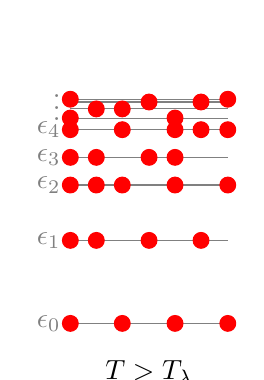
\begin{tikzpicture}
    \draw[gray] (2cm,0em) -- (0cm,0em) node[left] {$\epsilon_0$};
    \draw[gray] (2cm,3em) -- (0cm,3em) node[left] {$\epsilon_1$};
    \draw[gray] (2cm,5em) -- (0cm,5em) node[left] {$\epsilon_2$};
    \draw[gray] (2cm,6em) -- (0cm,6em) node[left] {$\epsilon_3$};
	\draw[gray] (2cm,7em) -- (0cm,7em) node[left] {$\epsilon_4$};
	\draw[gray] (2cm,7.42em) -- (0cm,7.42em) node[left] {$ $};
	\draw[gray] (2cm,7.75em) -- (0cm,7.75em) node[left] {$ $};
	\draw[gray] (2cm,8em) -- (0cm,8em) node[left] {$ $};
	\draw[gray] (2cm,8.1em) -- (0cm,8.1em) node[left] {$\vdots$};
	\draw[red,fill=red] (0.66cm,0em) circle (0.1cm);
	\draw[red,fill=red] (1.33cm,0em) circle (0.1cm);
	\draw[red,fill=red] (0cm,0em) circle (0.1cm);
	\draw[red,fill=red] (2cm,0em) circle (0.1cm);
	\draw[red,fill=red] (0cm,3em) circle (0.1cm);
	\draw[red,fill=red] (0.33cm,3em) circle (0.1cm);
	\draw[red,fill=red] (1cm,3em) circle (0.1cm);
	\draw[red,fill=red] (1.66cm,3em) circle (0.1cm);
	\draw[red,fill=red] (0cm,5em) circle (0.1cm);
	\draw[red,fill=red] (0.33cm,5em) circle (0.1cm);
	\draw[red,fill=red] (0.66cm,5em) circle (0.1cm);
	\draw[red,fill=red] (1.33cm,5em) circle (0.1cm);
	\draw[red,fill=red] (2cm,5em) circle (0.1cm);
	\draw[red,fill=red] (0cm,6em) circle (0.1cm);
	\draw[red,fill=red] (0.33cm,6em) circle (0.1cm);
	\draw[red,fill=red] (1cm,6em) circle (0.1cm);
	\draw[red,fill=red] (1.33cm,6em) circle (0.1cm);
	\draw[red,fill=red] (0cm,7em) circle (0.1cm);
	\draw[red,fill=red] (0.66cm,7em) circle (0.1cm);
	\draw[red,fill=red] (1.33cm,7em) circle (0.1cm);
	\draw[red,fill=red] (1.66cm,7em) circle (0.1cm);
	\draw[red,fill=red] (2cm,7em) circle (0.1cm);
	\draw[red,fill=red] (0cm,7.42em) circle (0.1cm);
	\draw[red,fill=red] (0.33cm,7.75em) circle (0.1cm);
	\draw[red,fill=red] (0.66cm,7.75em) circle (0.1cm);
	\draw[red,fill=red] (1cm,8em) circle (0.1cm);
	\draw[red,fill=red] (1.33cm,7.42em) circle (0.1cm);
	\draw[red,fill=red] (1.66cm,8em) circle (0.1cm);
	\draw[red,fill=red] (2cm,8.1em) circle (0.1cm);
	\draw[red,fill=red] (0cm,8.1em) circle (0.1cm);
	\draw (1cm,-1em) node[below] {$T>T_\lambda$};
    \end{tikzpicture}
    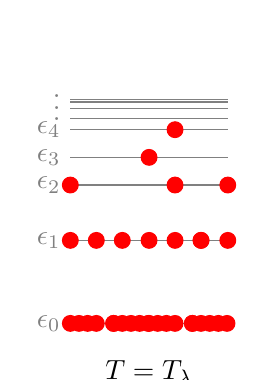
\begin{tikzpicture}
    \draw[gray] (2cm,0em) -- (0cm,0em) node[left] {$\epsilon_0$};
    \draw[gray] (2cm,3em) -- (0cm,3em) node[left] {$\epsilon_1$};
    \draw[gray] (2cm,5em) -- (0cm,5em) node[left] {$\epsilon_2$};
    \draw[gray] (2cm,6em) -- (0cm,6em) node[left] {$\epsilon_3$};
	\draw[gray] (2cm,7em) -- (0cm,7em) node[left] {$\epsilon_4$};
	\draw[gray] (2cm,7.42em) -- (0cm,7.42em) node[left] {$ $};
	\draw[gray] (2cm,7.75em) -- (0cm,7.75em) node[left] {$ $};
	\draw[gray] (2cm,8em) -- (0cm,8em) node[left] {$ $};
	\draw[gray] (2cm,8.1em) -- (0cm,8.1em) node[left] {$\vdots$};
	\draw[red,fill=red] (0cm,0em) circle (0.1cm);
	\draw[red,fill=red] (0.33cm,0em) circle (0.1cm);
	\draw[red,fill=red] (0.11cm,0em) circle (0.1cm);
	\draw[red,fill=red] (0.22cm,0em) circle (0.1cm);
	\draw[red,fill=red] (0.55cm,0em) circle (0.1cm);
	\draw[red,fill=red] (0.55cm,0em) circle (0.1cm);
	\draw[red,fill=red] (0.66cm,0em) circle (0.1cm);
	\draw[red,fill=red] (0.77cm,0em) circle (0.1cm);
	\draw[red,fill=red] (0.88cm,0em) circle (0.1cm);
	\draw[red,fill=red] (0.99cm,0em) circle (0.1cm);
	\draw[red,fill=red] (1cm,0em) circle (0.1cm);
	\draw[red,fill=red] (1.33cm,0em) circle (0.1cm);
	\draw[red,fill=red] (1.11cm,0em) circle (0.1cm);
	\draw[red,fill=red] (1.22cm,0em) circle (0.1cm);
	\draw[red,fill=red] (1.55cm,0em) circle (0.1cm);
	\draw[red,fill=red] (1.55cm,0em) circle (0.1cm);
	\draw[red,fill=red] (1.66cm,0em) circle (0.1cm);
	\draw[red,fill=red] (1.77cm,0em) circle (0.1cm);
	\draw[red,fill=red] (1.88cm,0em) circle (0.1cm);
	\draw[red,fill=red] (1.99cm,0em) circle (0.1cm);
	\draw[red,fill=red] (0cm,3em) circle (0.1cm);
	\draw[red,fill=red] (0.33cm,3em) circle (0.1cm);
	\draw[red,fill=red] (0.66cm,3em) circle (0.1cm);
	\draw[red,fill=red] (1cm,3em) circle (0.1cm);
	\draw[red,fill=red] (1.33cm,3em) circle (0.1cm);
	\draw[red,fill=red] (1.66cm,3em) circle (0.1cm);
	\draw[red,fill=red] (1.66cm,3em) circle (0.1cm);
	\draw[red,fill=red] (2cm,3em) circle (0.1cm);
	\draw[red,fill=red] (0cm,5em) circle (0.1cm);
	\draw[red,fill=red] (1.33cm,5em) circle (0.1cm);
	\draw[red,fill=red] (2cm,5em) circle (0.1cm);
	\draw[red,fill=red] (1cm,6em) circle (0.1cm);
	\draw[red,fill=red] (1.33cm,7em) circle (0.1cm);
	\draw (1cm,-1em) node[below] {$T=T_\lambda$};
  \end{tikzpicture}
  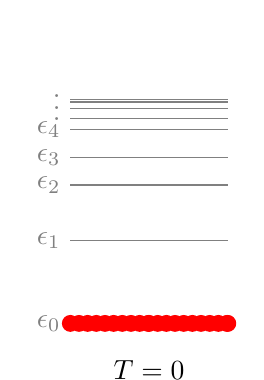
\begin{tikzpicture}
    \draw[gray] (2cm,0em) -- (0cm,0em) node[left] {$\epsilon_0$};
    \draw[gray] (2cm,3em) -- (0cm,3em) node[left] {$\epsilon_1$};
    \draw[gray] (2cm,5em) -- (0cm,5em) node[left] {$\epsilon_2$};
    \draw[gray] (2cm,6em) -- (0cm,6em) node[left] {$\epsilon_3$};
	\draw[gray] (2cm,7em) -- (0cm,7em) node[left] {$\epsilon_4$};
	\draw[gray] (2cm,7.42em) -- (0cm,7.42em) node[left] {$ $};
	\draw[gray] (2cm,7.75em) -- (0cm,7.75em) node[left] {$ $};
	\draw[gray] (2cm,8em) -- (0cm,8em) node[left] {$ $};
	\draw[gray] (2cm,8.1em) -- (0cm,8.1em) node[left] {$\vdots$};
	\draw[red,fill=red] (0cm,0em) circle (0.1cm);
	\draw[red,fill=red] (0.33cm,0em) circle (0.1cm);
	\draw[red,fill=red] (0.11cm,0em) circle (0.1cm);
	\draw[red,fill=red] (0.22cm,0em) circle (0.1cm);
	\draw[red,fill=red] (0.44cm,0em) circle (0.1cm);
	\draw[red,fill=red] (0.55cm,0em) circle (0.1cm);
	\draw[red,fill=red] (0.66cm,0em) circle (0.1cm);
	\draw[red,fill=red] (0.77cm,0em) circle (0.1cm);
	\draw[red,fill=red] (0.88cm,0em) circle (0.1cm);
	\draw[red,fill=red] (0.99cm,0em) circle (0.1cm);
	\draw[red,fill=red] (1cm,0em) circle (0.1cm);
	\draw[red,fill=red] (1.33cm,0em) circle (0.1cm);
	\draw[red,fill=red] (1.11cm,0em) circle (0.1cm);
	\draw[red,fill=red] (1.22cm,0em) circle (0.1cm);
	\draw[red,fill=red] (1.55cm,0em) circle (0.1cm);
	\draw[red,fill=red] (1.44cm,0em) circle (0.1cm);
	\draw[red,fill=red] (1.66cm,0em) circle (0.1cm);
	\draw[red,fill=red] (1.77cm,0em) circle (0.1cm);
	\draw[red,fill=red] (1.88cm,0em) circle (0.1cm);
	\draw[red,fill=red] (1.99cm,0em) circle (0.1cm);
	\draw[red,fill=red] (2cm,0em) circle (0.1cm);
	\draw (1cm,-1em) node[below] {$\phantom{T_\lambda}T=0\phantom{T_\lambda}$};
  \end{tikzpicture}
  \caption{\label{fig:beclevels}Schematic depiction of Bose-Einstein condensation. The ground state $\epsilon_0$ becomes macroscopically occupied as the temperature is reduced to below the critical temperature for condensation. In the limit of $T=0$ all bosons occupy the ground state.}
\end{figure}

Consider a gas of non-interacting bosons in thermal equilibrium at temperature $T$. The thermal de Broglie wavelength for each particle characterises the spatial extent of its localised wavepacket, and is conventionally defined by
\begin{equation}
\lambda_{\rm dB} = \sqrt{\frac{2\pi \hbar^2}{mk_{\rm B}T}},
\label{eq:debroglie}
\end{equation}
where $m$ is the mass of the particle and $\hbar$ is Plank's reduced constant. The de Broglie wavelength is inversely proportional to the square root of the temperature $T$, so that at high temperatures the wavepacket of each particle is small compared to the average inter-particle distance. Here classical, particle-like behaviour dominates the dynamics of the gas and the particles follow the classical Boltzmann distribution. As the temperature of the particles is reduced, the wavelength associated with the particles grows. At a critical temperature, $T_\lambda$, the wavelength for each particle becomes comparable to the average inter-particle distance and the individual characteristics of particles are no longer apparent. Here the particles become indistinguishable and the idea of a particle trajectory no longer makes sense. The particles now behave in a truly quantum manner, forming a degenerate gas. The critical temperature for which this process occurs marks the onset of Bose-Einstein condensation.

For a gas of identical non-interacting Bosons in a uniform three-dimensional system of volume $V$ and number density $n=N/V$, Bose-Einstein condensation occurs when $n\lambda_{\rm dB}^3 \leq \zeta(3/2)$ \cite{huang1987statistical,Pethick}, where $\zeta(3/2)\approx2.612$ is the Riemann zeta function evaluated at $3/2$. By using this relation with Equation \ref{eq:debroglie} one finds the critical temperature,
\begin{equation}
T_\lambda = \frac{2\pi\hbar^2}{mk_{\rm B}} \left ( \frac{n}{\zeta(3/2)} \right )^{2/3},
\label{eq:tlambda}
\end{equation}
for the onset of Bose-Einstein condensation. The fraction of bosons condensed into the ground state can then be calculated as a function of temperature,
\begin{equation}
	\frac{N_0}{N} = 1 - \left( \frac{T}{T_\lambda}\right )^{3/2}.
\end{equation}

\section{Superfluid helium}
Many concepts relating to Bose-Einstein condensation and quantum gases were developed in the context of liquid $^4$He. Liquid helium is interesting in that when cooled to very low temperatures, the liquid does not crystallise or solidify at atmospheric pressures. In fact a pressure of over $25$ atmospheres is required to solidify $^4$He, even at its lowest temperatures \cite{Pethick}. 

Around 1930, Keesom {\it et. al} \cite{Keesom27,Keesom35} observed that when cooling liquid $^4$He, there exists a critical temperature known as the lambda point ($T_\lambda = 2.17$ K) at which the fluid undergoes a phase transition into a state known as helium II. It was later discovered by Kapitza \cite{Kapitza}, Allen and Misener \cite{Allen38} that helium II exhibits inviscid flow (one of several remarkable properties of helium II), and the fluid was deemed a ''superfluid''.

London \cite{London38,London38b} was the first to interpret the properties of helium II as a manifestation of Bose-Einstein condensation of helium atoms, but the idea was not widely accepted at first. The strongly-interacting liquid of helium atoms is a world away from Einstein's non-interacting gas of bosons. Instead, the two-fluid model of Landau \cite{Landau41} was the first successful description of helium II hydrodynamics, wherein two fluids exist alongside one another with densities depending on the temperature: an inviscid superfluid component and a viscous normal fluid component. The superfluid component's density tents to zero as the temperature tends to the lambda point, and the normal fluid's density tends to zero as the temperature tends to zero.

\subsection{Dispersion relation and excitations}
Landau showed that superfluid behaviour can be accounted for by a dispersion relation that is linear at low momenta \cite{Landau41}. Bogoliubov then showed that a weakly-interacting Bose gas supports exactly such a dispersion law \cite{bogo47}. This link between bosonic gases and helium II was a strong indicator that Bose-Einstein condensation was indeed the fundamental mechanism behind superfluidity, and finally gave traction to London's theory. Onsager \cite{Onsager49} and Feynman \cite{Feynman55} then predicted quantised circulation as an extension to London's work.

\begin{figure}
	\centering
	\begin{tikzpicture}
		\begin{axis}[samples=300,ylabel near ticks,xlabel near ticks,
				width=0.4\linewidth,
				height=0.45\linewidth,
				xlabel=$p$,
				ylabel=$\epsilon$,
				xmin=0,
				xmax=13,
				ymin=0.4,
				ymax=12,
				axis line style={-Latex[round]},
				axis y line*=left,
        axis x line*=bottom,
        yticklabels={,,},
        xticklabels={,,},
				major tick length = 0.00cm]
				\addplot[mark=none,thick,domain=0:12] {x^(0.25)*((x/2-4)*sin(deg(x/2-4)) + 4)};
		\end{axis}
	\end{tikzpicture}%
	\caption{\label{fig:hedisp}The dispersion relation for superfluid $^4$He, demonstrating the spectrum of elementary excitations. The linear dispersion of phonons can be seen at at low momenta and the roton minimum at higher momenta.}
\end{figure}

The dispersion relation for liquid helium $^4$He is shown in Figure \ref{fig:hedisp}. For small momenta the relation is indeed linear. The fundamental excitations associated with this part of the relation are sound waves, known as {\it phonons}. For larger momentum, however, $\epsilon(p)$ exhibits an approximately quadratic shaped dip and local minimum. The fundamental excitations of this part of the relation are known as {\it rotons}, with the centre of the dip corresponding to the smallest possible energy of a roton, the {\it roton minimum}. 

While Bose-Einstein condensation is now known to be the driving force behind helium II superfluidity, the strong interactions inherent in liquid helium restricts the condensed fraction of helium atoms to less than $10\%$ \cite{Donnelly} (even in the limit of zero temperature) and so a weakly-interacting Bose gas provides only a qualitative model of helium II superfluidity.

\section{Dilute weakly-interacting atomic gases}
Gases of alkali atoms such as rubidium, sodium and lithium are ideal candidates for condensation: they are weakly-interacting, can be easily trapped magnetically, and readily cooled using lasers. When considering these gases, Einstein's ideal gas predictions provide a good estimate of the critical temperature for Bose-Einstein condensation.  However, as the gas is cooled towards the critical temperature it is necessary to avoid the transition into a liquid or solid. This can be done by reducing the atomic density such that the gas is dilute enough that elastic binary collisions in the gas dominate over three-body collisions. The required atomic densities are around $n \sim 10^{14}~{\rm cm}^{-3}$ \footnote{Compare this to the density of dry air at room temperature, $n \sim 10^{19}~{\rm cm}^{-3}$.}, and so by using Equation \ref{eq:tlambda} one predicts that the ultra-low temperatures of $T \sim 10^{-6}~{\rm K}$ are required for the onset of Bose-Einstein condensation.

\subsection{Experimental realisation}
The requirement of such low temperatures delayed the realisation of a true atomic BEC until 1995, when advances in atom cooling and trapping \cite{billphillips,chu98,Cohen-Tannoudji} lead to the condensation in vapours of rubidium ($^{87}$Rb) by the group of Professors Carl Wieman and Eric Cornell at the University of Colorado \cite{Anderson198}, and sodium ($^{23}$Na) by the group of W. Ketterle at MIT \cite{PhysRevLett.75.3969}. Wieman, Cornell and Ketterle were awarded the 2001 Nobel Prize in Physics for ``{\it the achievement of Bose-Einstein condensation in dilute gases of alkali atoms, and for early fundamental studies of the properties of the condensates}'' \cite{nobel01}.

A variety of cooling techniques, including laser \cite{billphillips,chu98,Cohen-Tannoudji} and evaporative \cite{PhysRevB.34.3476} cooling developed in the attempt to condense spin-polarised hydrogen \cite{Hecht59, PhysRevLett.44.164, Silvera86}, are used to reach the ultra-low temperatures required for atomic Bose-Einstein condensation \cite{Pethick,RevModPhys.74.1131,RevModPhys.74.875}. A typical atomic condensate begins life as around $10^9$ atoms which are cooled to around 1K by a Zeeman slower: a laser beam propagating opposite to the atom flow reduces the velocity of the atoms from around $800~\rm{m/s}$ to $30~\rm{m/s}$. The atoms are transferred to a magneto-optical trap (MOT) formed by laser beams and magnetic fields and further cooled through Doppler cooling, where the Doppler effect is employed to reduce the momentum of atoms. A limit of this method is reached at around $1\,\mu$K \cite{Pethick} at which point evaporative cooling is required to cool the gas even further. Here the confining trap is carefully modified so that the high energy atoms escape the system. The remaining lower energy atoms rethermalise at a reduced temperature and lower density due to the loss of atoms. Using this technique, the gas can be cooled to the nK regime. The BEC then emerges marked by a spike at the zero of the velocity distribution for the atoms, indicating a macroscopic occupation of the ground state. 

Since the first experiments in 1995, an explosion of ultra-cold atomic physics has followed. Many species of atom are now routinely condensed by over 50 experimental groups all over the world. The list grows continuously: many alkalis \cite{Anderson198,PhysRevLett.75.3969,PhysRevLett.75.1687,PhysRevLett.78.985,PhysRevLett.85.1795,Modugno,Robert461,Weber232}, calcium \cite{PhysRevLett.103.130401}, dysprosium \cite{PhysRevLett.107.190401}, strontium \cite{PhysRevLett.103.200401,PhysRevLett.103.200402, PhysRevA.82.041602, PhysRevA.81.051601}, ytterbium \cite{PhysRevLett.91.040404}, chromium \cite{PhysRevLett.94.160401}, spin-polarised hydrogen \cite{PhysRevLett.81.3811}, metastable helium \cite{PhysRevLett.86.3459}, magnons \cite{Mathew11}, exciton-polaritons \cite{Kasprzak06} and even mixtures of different species \cite{PhysRevLett.89.053202, PhysRevLett.89.190404, PhysRevLett.100.210402,PhysRevA.84.011603}. Each expanding the richness of fascinating phenomena available to experimentalists, with their unique atomic properties and range of interactions.

The experimental advances of controlling the trapping potential has allowed for direct interaction with the condensate using time-dependent magnetic fields and lasers. Localised laser beams can punch a `hole' in a condensate to create almost arbitrarily shaped obstacles \cite{Henderson09}. Exotic trapping potentials such as ring traps \cite{persistent,Ramanathan11}, uniform box traps \cite{gaunt_2013,chomaz_2015}, optical lattices \cite{Greiner02} and double-well \cite{PhysRevLett.106.025302} potentials can be realised with relative ease. The route has even opened to experimentation in reduced dimensionality \cite{Gorlitz,PhysRevLett.87.080403,PhysRevLett.91.250402,PhysRevLett.92.173003}. By significantly trapping the gas alone one dimension it is possible to make a disc shaped, effectively two dimensional condensate, useful \cite{Neely,Freilich2010} for the study of vortex dynamics. A further trapping along a second dimension creates an elongated, effectively one dimensional condensate such that solitons are stable.

\subsection{Scattering length and interactions}
The atomic binary collisions in dilute gases are characterised by the $s$-wave scattering length, $a_s$. Higher energy $p$-wave and $d$-wave scattering is suppressed. Geometrically, a positive $a_s$ (as in a rubidium or sodium BEC) can be thought of as a measure of the effective radius of repulsive atoms. For gases with density in the region required, $n^{1/3}a_s \ll 1$, and so $a_s$ is much smaller than the average inter-atomic distance. This implies that the gas is weakly-interacting and around $99\%$ of the atoms can become Bose-condensed, resulting in a condensate fraction much greater than the theoretical maximum for helium II. This makes ultra-cold dilute atomic gases the purest form of BEC that can also be easily controlled and manipulated in the lab.

The scattering length may also be negative (as in a lithium BEC \cite{PhysRevLett.75.1687, PhysRevLett.78.985}), in this case the atoms are attractive, rather than repulsive, and the BEC is only stable up to a certain atom number. Importantly, it is possible to control the inter-atomic interaction, and therefore the scattering length, through the entire range of the parameter space using techniques such as {\it Feshbach resonance} (theoretically laid out in \cite{weiner2003cold} and experimentally demonstrated in \cite{Inouye1998,PhysRevLett.82.2422,PhysRevLett.85.1795}), providing further experimental control over BEC dynamics.

With the unique level of purity and control available in the lab, weakly-interacting dilute atomic gases have become the ideal test-bed for studying Bose-Einstein condensation and for observation of quantum effects on a macroscopic scale.


\section{Macroscopic nonlinear excitations: vortices and solitons}
The rise of interest in Bose-Einstein condensation has lead to a great amount of theoretical work. It can be argued that the greatest success in this area is the development of an effective mean-field theory which provides the so-called Gross-Pitaevskii equation (GPE) \cite{Pethick,Pitaevskii61,Gross61,RevModPhys.71.463}, a classical evolution equation and a variant of the nonlinear-Schr\"oedinger equation used in many areas of physics, including plasmas and optics. The GPE is much simpler than modelling a BEC using the full many-body Schr\"oedinger equation, yet accurately captures the statics and dynamics \cite{Denschlag97, Burger99, PhysRevLett.86.2926, Dutton27072001} of a BEC over a range of realistic experimental parameters. Section \ref{cha:theoretical_model} describes the mean-field formulation  in detail and formally derives the GPE from the starting point of the many-body Schr\"oedinger equation.

The non-linearity in the GPE arises from atom-atom interactions and gives rise a great deal of interesting effects, both from a mathematical standpoint and when applied to an atomic BEC. A selection of the interesting and experimentally relevant nonlinear phenomena are described in this section.

\subsection{Vortices}
One of the non-linear excitations supported by the GPE is {\it quantum vortices}, which arise via topological defects in the wavefunction that parametrises the condensate. Solutions with quantum vortices contain structures identified by a localised density dip, the vortex core, masking a phase singularity in its centre. The phase singularity forms a velocity field such that fluid circulates around the vortex core.

Quantum vortices are carriers of vorticity in an irrotational superfluid system, and can arise naturally during the formation of a BEC or by directly interacting with a condensate using magnetic fields or lasers. A standard method of generating vortices, relevant to condensates and helium II, is by rotation of the superfluid. At lower angular speeds the rotation has no effect, however, past a critical value the presence of vortices lowers the energy of the system. In this case, one or more vortices nucleate into the system. The nucleated vortices form a lattice in the centre of the system. Another example is the formation of vortices as a result of broken symmetry after a fast quench into the BEC regime. Through the Kibble-Zurek mechanism, pockets of phase coherence form, separated in space. As the phase coherence grows in the condensate, boundaries are created and discontinuities along these boundaries leads to the formation of vortex lines. Further methods of generating vortices include artificial phase imprinting of the topological defect via laser light, or by stirring a BEC with a localised laser beam.

Quantised vortices have much in common with the classical vortices observed at many scales in nature. However, while classical vortices can be created with any degree of fluid rotation, characterised by the circulation $\Gamma$, quantised vortices differ in that their circulation is constrained (as a direct consequence of quantum mechanics) to integer multiples of the {\it quantum of circulation}, $\kappa$, with a value dependent on the system.

Experimentally, quantum vortices have been realised in many different configurations and for various dimensionality. In three-dimensions vortex lines, vortex rings and even tangles of vortices have been observed in BECs. In quasi-two-dimensional BECs, quantum vortices have been realised from the level of a single vortex, as vortex pairs and dipoles, through to many vortices of mixed circulation in turbulence. There has also been observation of vortex lattices, giant vortices, and multiply charged vortices in condensates with a variety of trap geometries.

Quantum vortices have also been observed in superfluid helium. In 1979, the first clear and direct image of a quantised vortex lattice in rotating helium II was provided by Packard {\it et. al}. Here electrons were trapped inside vortex cores and accelerated towards a florescent screen to mark the position of the vortex. The resulting images are shown in Figure {\ref{fig:hevorts}} for different rotation speeds.

\begin{figure}
\includegraphics[width=\linewidth]{intro/packard}
\caption{\label{fig:hevorts} Results of the superfluid helium experiments of Packard, with (a-l) corresponding to increasing rotation velocities of the helium II container. Vortex line position is marked by the glowing dots.}
\end{figure}

\subsection{Solitons}
Solitons are a non-linear localised excitation, supported by the one dimensional GPE. Soliton solutions contain localised propagating wavepackets that are self-reinforcing due to the non-linearity of the system balancing dispersive effects. When in a homogeneous medium they travel at zero or finite constant speed, and have the property that they undergo non-destructive collisions. There are two species of soliton that we consider, bright and dark solitons. Their behaviour in optics, leading to a bright collection or dark absence of light, is the origin of these names. Solitons are an active area of research in several diverse areas of non-linear mathematics and physics, and are well known for their applications in optical and fluid systems.

For these reasons solitons have been of great interest since the first experimental realisation of atomic BECs. In three-dimensional BECs, solitons take the form of solitonic waves, but are not solitons in the strict mathematical sense; the structures are unstable and proceed to decay. In weakly-interacting BECs with quasi-1D geometries, however, solitons are stable and have been observed with long lifetimes and in agreement with numerical simulations.

\subsubsection{Bright solitons}
Bright solitons arise in fluid, plasma, acoustical, and optical physics and can be easily pictured by the classical example of a hump travelling along the surface of shallow water, as first reported in 1845. The non-dispersal and destruction-less collision properties of bright solitons make them particularly important in applications for optical communications.

Bright solitons are supported in condensates for the case of effectively attractive interactions ($a_s < 0$), and have been generated and experimentally observed in lithium in a quasi-one-dimensional optical trap.

\subsubsection{Dark solitons}
In general, dark solitons are less prevalent than the bright species, but are of particular interest in the context of weakly-interacting BECs as they are are formed in the case of repulsive interactions ($a_s > 0$). They consist of a density dip and phase slip of varying size, depending on the speed of the soliton propagation. Dark solitons were first realised in 1987 in the context of non-linear optics, followed by their creation in shallow liquids, as discrete mechanical standing waves, and in magnetic films.

More recently, dark solitons have been engineered in repulsive atomic BECs in a controlled manner through phase imprinting methods and by perturbing the condensate density. They have also been produced through dynamical processes, in one case by sweeping a repulsive barrier, generated via a laser beam, through the condensate.

Dark solitons that have been generated in higher than quasi-1D geometries have been observed to decay into vortex rings, due to their known instability to transverse excitations.


\section{Quantum turbulence}
Classical turbulence is a complicated flow regime characterised by chaotic and highly irregular flow and the appearance of unsteady vortices on many length scales interacting with one another. In classical isotropic turbulence, most of the kinetic energy is contained in large-scale structures and is distributed following the famous Kolmogorov energy spectrum.

{\it Quantum} turbulence is a state dominated by an irregular tangle of quantised vortex lines. The quantised circulation and inviscid flow characteristics of superfluidity provides a simplified platform to study complicated vortex dynamics in general, and so the nature of turbulence in superfluids is the subject of much experimental and theoretical study. Despite the fundamental differences between superfluids and classical fluids, the observations of Kolmogorov energy spectra in superfluid turbulence are suggestive of a deep connection between them. 

\subsection{Turbulence in helium II}
Quantum vortices are carriers of vorticity in superfluids and play an important role in the behaviour of the superfluid component of helium II. They have been experimentally and theoretically studied in helium II from around 1950, but clearly visualising individual vortex lines within a tangle still provides a challenge in the present day. The large normal fluid component and a vortex core size of only a few Angstr\"oms limits visualisation techniques.

A large disordered collection of vortex lines is thought to be the driving force of the turbulence. However, within the tangle the vortex core size is small compared to the average inter-vortex spacing. For this reason the standard method of modelling of vortex dynamics at large-scales is handled by approximating the vortices as infinitesimally thin vortex filaments, with motion described by the Biot-Savart law. The limitation of the vortex filament model is that all phenomena that occur on the length-scale of the vortex core (of which we are interested in) is lost. Features like vortex reconnection can be manually introduced into this model, but the full microscopic description is lost.

On the other hand, the GPE model for a weakly-interacting Bose gas provides a microscopic model of helium II on a qualitative level. As already discussed, the strongly-interacting helium atoms, existence of high momenta rotons, and relatively low fraction of condensed atoms limits the accuracy of the model. Nevertheless, the GPE excels at describing the micro-scale phenomena such as vortex nucleation and reconnection, sound emission, and Kelvin wave excitation, and so we will use the GPE throughout this thesis to model helium II dynamics.

Typically turbulence in helium II is generated using mechanical methods, creating turbulence with oscillating obstacles, including grids, wires, spheres and others, or by rotation of the container. Non-mechanical methods have been also been devised, such as using ion bubbles or thermal counterflow to generate turbulence. It is understood that a mutual friction exists between the normal and superfluid components of the fluid, which leads to a dissipation of the vortex tangle in the superfluid at finite temperatures. In the limit of very low temperatures the mutual friction tends to zero. It is expected that in this limit Kelvin wave excitations and vortex reconnections leads to dissipation via sound waves, but the entire mechanism is not yet fully understood.

\subsection{Turbulence in BECs}

Weakly interacting atomic BECs present a key improvement over helium II superfluidity for the study of quantum turbulence. Although the spatial extent of BECs support much fewer vortices than for superfluid helium, the structure of individual vortices and their turbulent dynamics can be experimentally resolved much easier. This is due to the relatively large vortex core size, on the scale of a micron, available to atomic BECs and the fact that BECs can be readily visualised through imaging techniques so that the state of the entire atomic gas can be probed. Expansion imaging has provided a technical leap in this area, allowing individual vortex cores to be directly observed [Madison  2000;  Raman  2001]. Improved real time and non-destructive imaging of condensates has also recently been made available [Freilich 2010] allowing for observation of turbulent vortex trajectories. A further recent improvement in this area has allowed for the imaging of vortex polarity, as well as its location in space. These technical leaps in imaging have made atomic condensates an extremely attractive medium for exploiting quantum vortex dynamics and turbulence. 

The range of length scales available to classical turbulence and superfluid helium turbulence far outshines those currently available to atomic BECs, and much theory of classical turbulence is defined by the distribution of kinetic energy over the large number of length scales available. Nevertheless, numerical studies show quantum turbulence can distribute the kinetic energy in a condensate in agreement with Kolmogorov's $k^{-5/3}$ law (Nore, 1997; Berloff Svistunov, 2002;Kobayashi Tsubota, 2005; Yepez, 2009).



\end{chapter}

  \begin{chapter}{\label{cha:theoretical_model}Theoretical Modelling of BEC}
\section{\label{section:meanfield} Mean-field description}
We aim to accurately model the dynamics of a closed system containing a dilute, weakly interacting Bose gas of $N$ atoms, at extremely low temperatures. One could model the entire system by constructing a N-body quantum wavefunction, which would follow the Schr\"odinger equation, but the complexity of this method makes it extremely unwieldy to model the large number of particles used in Bose-Einstein condensate (BEC) experiments happening all around the world.

We instead model the system with a mean-field theory, in which there are essentially two main approximations. Firstly, justified by the dilute property of the gas, any binary interaction between particles is assumed to be a contact delta function,
\begin{equation*}
V(\mathbf{r}-\mathbf{r}') = g \delta(\mathbf{r}-\mathbf{r}').
\end{equation*}
Interactions involving a higher number of particles are ignored. Secondly, we assume all particles in the condensate are macroscopically described by a single wavefunction, $\psi(\mathbf{r},t)$. As the particles all share the same phase and quantum state, $\psi(\mathbf{r},t)$ is a classical field. This second approximation also assumes that there are no particles contributing to thermal or quantum fluctuations beyond the classical field, and so is only strictly justified when the temperature, $T$, is exactly $0\mathrm{K}$.

\section{\label{section:gpe} The Gross-Pitaevskii Equation}
The result of this methodology is the Gross-Pitaevskii equation (GPE), 
\begin{equation}
\mathrm{i} \hbar \frac{\partial\Psi({\bf r},t)}{\partial t} = \left(-\frac{\hbar^2}{2m}\nabla^2 + V({\bf r},t) + g|\Psi({\bf r},t)|^2 - \mu \right) \Psi({\bf r},t),
\label{eq:gpe}
\end{equation}
where $V({\bf r},t) = V_{\mathrm{obj}}({\bf r},t) + V_{\mathrm{trap}}({\bf r},t)$. When trapped, the trap is harmonic and of the form $V_{\mathrm{trap}}({\bf r},t)=m\omega^2r^2/2$, otherwise $V_{\mathrm{trap}}({\bf r},t)=0$.

Taking into account the fact that the GPE is only valid at $T=0$, it turns out the equation is surprisingly successful at quantitatively modelling ultra-cold gasses, even up to a temperature of $T=\frac{T_c}{2}$, where $T_c$ is the critical temperature for Bose-Einstein condensation. The GPE is also successful at qualitatively modelling BEC based effects in higher temperature superfluids, such as liquid helium II.

A detailed explanation of the mean-field formulation of the model and the full derivation of the GPE is shown in Section \ref{appsection:gpeqft}.

\section{\label{section:quasi2dgpe} Quasi-Two-Dimensional Gross-Pitaevskii Equation}
	When $\omega_z >> \omega_r$ and $\hbar\omega_z >> \mu$ the condensate becomes highly oblate. Tight $z$ confinement causes the dynamics to become essentially two dimensional.
	In this case a 2DGPE can be used to model the system where $g_{2D} = g/\left( \sqrt{2\pi}l_z\right )$. [CITE PARKER THESIS] The chemical potential is also modified. See Section \ref{section:mu} for details on $\mu$.

	To effectively reduce the system to two-dimensions, the BEC is assumed to be confined by a harmonic trapping potential in the axial ($z$) direction, $V(z)=\frac{1}{2}m \omega_z^2 z^2$, where $m$ is the atomic mass.  For sufficiently strong trapping, which requires $\hbar \omega_z \gg \mu$, where $\mu$ is the chemical potential of the 3D condensate, the axial wavefunction becomes ``frozen" into the time-independent harmonic oscillator ground state $\pi^{-1/4} l_z^{-1/2} \exp\left(-z^2/2l_z^2\right)$, where $l_z=\sqrt{\hbar/m \omega_z}$ is the axial harmonic oscillator length. Under these conditions, the condensate becomes effectively two-dimensional, as achieved experimentally \cite{Gorlitz}.  It is then described by an 2D GPE, corresponding to Equation (\ref{eq:gpe1}) with $g \rightarrow g/2\pi l_z^2$ and where $\Psi$, ${\bf r}$, $V$ and $n$ become two-dimensional quantities.  

\section{\label{section:gpedimless} Dimensionless Gross-Pitaevskii Equations}
	Bose-Einstein condensates can be formed with almost any size or scale. An ultra-cold BECs topology or atom interaction strength can be fairly easily changed with magnetic/optical potentials and Feshbach resonances. Superfluid helium can have vortex core sizes of $\sim$1 or $\sim$100 angstroms, depending on the isotope of helium used. The cores of neutron stars are even theorised to be superfluid. For this reason, it is desirable to rescale the length scales used in the GPE so that any of the calculations performed can be easily reformulated into any length scale desired. We make this process easier by doing all calculations with dimensionless parameters. 
	\subsection{\label{section:gpedimlesshomg} Homogeneous GPE}
		When discussing a homogeneous condensate we drop the dimensionless modifiers for each quantity and use the equation,
		\begin{equation}\label{eq:dimgpehomg}
		\mathrm{i}\frac{\partial\psi({\bf r},t)}{\partial t} = \left( -\frac{1}{2}\nabla^2 + |\psi({\bf r},t)|^2 + V_{\mathrm{obj}}({\bf r},t) - 1 \right) \psi({\bf r},t).
		\end{equation}
	\subsection{\label{section:gpedimlesstrap} Trapped GPE}
		When discussing the a trapped condensate we drop the dimensionless modifiers for each quantity and use the equation,
		\begin{equation}\label{eq:dimgpetrapped}
		\mathrm{i}\frac{\partial\phi({\bf r},t)}{\partial t} = \left( -\frac{1}{2}\nabla^2 + g|\phi({\bf r},t)|^2 + V({\bf r},t) - 1 \right) \phi({\bf r},t).
		\end{equation}
		Where $V({\bf r},t) = \frac{r^2}{2} + V_{\mathrm{obj}}({\bf r},t)$

\section{\label{section:dgpe} The Dissipative Gross-Pitaevskii Equation}
	\subsection{\label{section:gamma} Phenomenological dissipation}
	The GPE can be modified to provide a simple phenomenological model of a condensate's interaction with the thermal cloud. The phenomenological damping term, $\gamma$, is added to the right hand side of the GPE with the effect that the energy in the system no longer remains constant. The energy will instead vary over time to approach some constant value. This has the effect of damping out any excitations made to the condensate, and over time the wavefunction approaches the steady state. A microscopic justification for this model was provided by Penckwitt et al [CITE] and Gardiner at al [CITE]; by studying the growth of a condensate in the presence of a rotating thermal cloud an expression for $\gamma$ was found.
		\begin{equation}\label{eq:dissgamma}
		\gamma = \frac{4m\tilde{g}a^2kT}{\pi\hbar^2} \approx 0.01,
		\end{equation}
	where $k$ is Boltzmann's constant and $\tilde{g} = 3$ is a factor used for correction. As $\gamma$ is proportional to temperature, in this thesis various values of $\gamma$ will be used as a qualitative probe of finite-temperature dynamics with only marginally more complex numerical methods.
	In the case with a homogeneous condensate this leaves us with
		\begin{equation}\label{eq:dissgpehomg}
		(\mathrm{i} - \gamma)\frac{\partial\psi({\bf r},t)}{\partial t} = \left( -\frac{1}{2}\nabla^2 + |\psi({\bf r},t)|^2 + V_{\mathrm{obj}}({\bf r},t) - 1 \right) \psi({\bf r},t),
		\end{equation}
	and in the case with a trapped condensate this leaves us with
		\begin{equation}\label{eq:dissgpetrapped}
		(\mathrm{i}-\gamma)\frac{\partial\phi({\bf r},t)}{\partial t} = \left( -\frac{1}{2}\nabla^2 + g|\phi({\bf r},t)|^2 + V({\bf r},t) - 1 \right) \phi({\bf r},t).
		\end{equation}

	\subsection{\label{section:mu} The role of the chemical potential}
\section{\label{section:hydrodynamic} Hydrodynamic interpretation}
	Often it can be helpful to write the GPE, via the so called Madelung transformation, as a set of hydrodynamic equations. The transformation reinterprets the wavefunction $\Psi$ as a magnitude directly related to the fluid density and a phase which is directly related to the fluid velocity. We write the wavefunction in the form
	\begin{equation}
		\Psi({\bf r},t) = R({\bf r},t)\exp (\mathrm{i}\theta({\bf r},t)),
	\end{equation}
	 and identify the fluid density as $\rho=mR^2$ and the velocity as $\mathbf{v} = \frac{\hbar}{m}\nabla\theta$.
	In vector form we obtain a continuity equation
	\begin{equation}
	  \frac{\partial \rho}{\partial t} + \nabla(\rho{\bf v}) = 0,
	  \label{eq:MTcont}
	\end{equation}
	and an equation similar to the Euler equation for an inviscid fluid,
	\begin{equation}
	\rho\left( \frac{\partial \mathbf{v}}{\partial t} + \left( \mathbf{v} \cdot \nabla \right)\mathbf{v} \right) = -\nabla p - \nabla \mathbf{P} - \rho \nabla \left(\frac{V}{m}\right).
	\end{equation}
	where $P_{jk} = -\frac{\hbar^2}{4m^2}\rho\frac{\partial^2\ln{\rho}}{\partial x_j \partial x_k}$.
	A detailed derivation of this result can be found in Appendix \ref{appsection:madtrans}.

\section{\label{section:solutions} A selection of analytical solutions}
	\subsection{\label{section:wall} Density near a wall}
	\subsection{\label{section:soliton} Soliton solutions}
		\begin{equation}
		\Psi(x) = \Psi_0 \tanh \left( \frac{x}{\sqrt{2}\xi} \right)
		\label{eq:soliton}
		\end{equation}
	\subsection{\label{section:vortices} A note on vortex solutions}
\section{\label{section:inital} Initial Conditions}
	\subsection{\label{section:tftrap} Thomas Fermi profile of a trapped condensate}
	Fixed in time $\Psi$ and $V$.
	\begin{equation}
	\sqrt{\frac{\mu - V({\bf r})}{g}} =  \Psi({\bf r})
	\label{eq:TF}
	\end{equation}
	\subsection{\label{section:cfield} Classical Field approximation with a homogeneous condensate}
		\begin{equation}
		\psi({\bf r},t) = \sum_{\bf k} a_{\bf k} \exp (\mathrm{i}{\bf k}\cdot{\bf r}),
		\label{eq:cFieldIC}
		\end{equation}
		where the complex Fourier amplitudes $a_{\bf k}$ are related to the occupation numbers $n_{\bf k}$ through $\braket{a_{\bf k}^{\,}a_{\bf k'}^*} = n_{\bf k}\delta_{\bf kk'}$. The phase of the complex amplitudes $a_{\bf k}$ are distributed uniformly on $[0,2\pi]$ while $|a_{\bf k}|$ is distributed randomly with fixed mean equal to unity; it has been found that different distributions of $|a_{\bf k}|$ make no qualitative difference to the turbulent evolution[phys rev A 66 013603]. [TODO: write about choice of E and N here to get different condensate fractions]

		We also have the integral distribution function,
		\begin{equation}
		D_k = \sum_{k'<k}n_{\bf k}.
		\label{eq:intDistFunc}
		\end{equation}
		This is a coarse-grained characteristic of the particle distribution which shows how many particles have momenta less than $k$.

\section{\label{section:potentials}Creating obstacles with repulsive potentials}

\subsection{\label{section:3dobjpotential} Three-dimensional elliptical Gaussian}
In our 3D simulations, we solve the 3D GPE of Equation (1), where the localized 3D obstacle is modelled via a repulsive ellipsoidal Gaussian potential,
\begin{equation}
V({\bf r}, t)=V_0 \exp \left( -\frac{\varepsilon^2(x-x_0-vt)^2}{d^2} -\frac{(y-y_0)^2}{d^2}-\frac{(z-z_0)^2}{d^2}\right),
\label{eq:potential3D}
\end{equation}
where  $V_0$ is its (constant) amplitude, $d$ its width in the $y$ and $z$ directions, and $(x_0,y_0,z_0)$ its initial coordinates.  

\subsection{\label{section:3dcylinderpotential} Three-dimensional cylindrical Gaussian}
\subsection{\label{section:3dafmpotential} Three-dimensional `realistic' rough-surface}
\subsection{\label{section:2dobjpotential} Two-dimensional Gaussian}

In 2D, we model the obstacle via a moving repulsive Gaussian potential of the form,
\begin{equation}
V({\bf r}, t)=V_0 \exp \left( -\frac{\varepsilon^2(x-x_0-vt)^2}{d^2} -\frac{(y-y_0)^2}{d^2}\right).
\label{eq:potential2D}
\end{equation}




\subsection{\label{section:2dbitmappotential} Two-dimensional arbitrary bitmap}
\section{\label{section:movingframe} An alternative reference frame }
	The GPE is transformed into the reference frame moving with the obstacle (in $x$) via the addition of the Galilean term $ i\hbar v\frac{\partial}{\partial x} \Psi$ to the right-hand side of the GPE (\ref{eq:gpe1}), where $v$ is the frame velocity. 
\end{chapter}

  \begin{chapter}{\label{cha:numerics}Numerical Algorithms}
\section{\label{section:RK} Numerical procedures for 2D and 3D solutions}
	\subsection{\label{section:RK4} Fourth order Runge-Kutta scheme}
	The classical fourth-order Runge-Kutta formula (RK4) is described equivalently in many texts. We follow the description in \cite{NumericalRecipes}. Let an initial value problem be specified as
	
	\begin{align*}
		\frac{\partial \psi}{\partial t} &= f(\psi,t),\hspace{0.25in}\psi(t_0) = \psi_0.
	\end{align*}

A step-size, $h>0$, is chosen as the parameter controlling how the solution is advanced over $t$. The scheme for estimating $\psi(t_n)= \psi_n$ is then written
\begin{equation}
\begin{split}
		k_1 &= hf(t_n,\psi_n),\\
		k_2 &= hf(t_n+\frac{h}{2},\psi_n+\frac{k_1}{2}),\\
		k_3 &= hf(t_n+\frac{h}{2},\psi_n+\frac{k_2}{2}),\\
		k_4 &= hf(t_n+h,\psi_n+k_3),\\
		\psi_{n+1} &= \psi_n + \frac{k_1}{6}+ \frac{k_2}{3}+ \frac{k_3}{3} + \frac{k_4}{6} + O(h^5),\\
		t_{n+1}  &= t_n + h.
		\label{eq:rk4}
\end{split}
\end{equation}


	A full derivation and proof of accuracy for the RK4 scheme is outlined in Appendix \ref{appsection:rk4deriv}.
	In all of our relevant calculations the value of f is set as the right hand side of the homogeneous or trapped GPE. The main loop formulating the RK4 method may be repeated indefinitely to reach any $t>t_0$. The step size for a given set of parameters should be chosen small enough that smaller choices make no quantitative changes to the resulting solution.

	\subsection{\label{section:numericalParams} Numerical stability}
	We now systematically study the numerical stability of common simulated systems. Our aim is to find a suitable discretisaton of space and time so that while simulations are timely, our numerical solutions are converged and not overly sensitive to small changes computational parameters.

	We use energy to measure because in the undamped gpe energy is conserved.

	We run 100 units of imaginary time stepping to get density profile
	We run another 100 units for vortex IC
	We run 500 units in real time to study stability


\begin{figure}
	\centering
	\includegraphics[width=0.5\textwidth]{numerics/figures/homg_energy_cons.png}
\end{figure}

\section{\label{section:vortexidentifying} Identifying vortices}


\subsection{\label{section:gaussianblur} Image filters and the Gaussian kernel}

\section{\label{section:vortexclustering} Quantifying vortex clustering}
	\subsection{\label{section:reevesalgorithm} Recursive Cluster Algorithm (RCA) }
		


	\subsection{\label{section:ripleysk} Ripley's K function }
		\begin{equation}\label{eq:ripleysk}
		K(x) = \frac{A}{n^2}\sum\limits_{i \ne j} I\left (d_{ij}<x\right ),
		\end{equation}
		where $d_{ij}$ is the distance between the $i$th and $j$th points, $A$ is the area of the region containing every point, $n$ is the number of points, $x$ is the search radius, and I is the indicator function (1 if its argument is true, 0 otherwise). Should the points be distributed homogeneously in space, then $K(s)\approx\pi s^2$.
\section{\label{section:vortextracking} Tracking vortex trajectories}
\section{\label{section:vortexremoval} Removing vortices with phase unwrapping}
	

\end{chapter}

  \part{Numerical Studies}
  \begin{chapter}{\label{cha:wake}Classical-like wakes behind elliptical obstacles in Bose-Einstein condensates}

\section{Introduction}
\begin{figure}[!ht]
\centering
  \includegraphics[height=2.08cm,angle=180]{wake/3.png}
  \includegraphics[width=0.24\textwidth,angle=180]{wake/taneda41}
  \includegraphics[width=0.24\textwidth,angle=180]{wake/taneda112}
    \includegraphics[width=0.29\textwidth,angle=180]{wake/turb.jpg}
  \caption{Classical viscous flow past a cylinder. From left to right: laminar flow ($\Rey=3.64$) \cite{taneda41}; steady symmetric wake behind the cylinder ($\Rey=41$) \cite{taneda41}; time-dependent B\'enard--von K\'arm\'an vortex street ($\Rey = 112$) \cite{taneda112}; and chaotic downstream wake ($\Rey > 10^5$) \cite{nagib}.} 
  \label{fig:taneda-imgs}
\end{figure}
Recent experimental \cite{Tabeling,Salort}, 
numerical \cite{Nore,Kobayashi,Laurie} 
and theoretical studies \cite{Lvov}
have highlighted similarities between turbulence in quantum
fluids and turbulence in ordinary (classical) fluids \cite{Frisch}.
In particular, it is found that, in
the idealized case of homogeneous isotropic conditions away from
boundaries, the distribution of kinetic energy over the 
length scales obeys the celebrated Kolmogorov scaling of 
classical turbulence \cite{barenghi}. This similarity is remarkable,
because a superfluid has zero viscosity and vorticity is not a continuous
field. In the more realistic presence of boundaries such as an obstacle or confining channel
walls, superfluid hydrodynamics is less understood, despite the large number of experiments in such scenarios. 

In a classical viscous fluid \cite{Frisch}, the prototype problem with
a boundary is the flow 
around a cylinder or a sphere (or, changing the frame of reference, 
the motion of a cylinder or a sphere in a fluid at rest).
The nature of such flow is determined by the Reynolds 
number $\Rey = vd/\nu$, where $v$ is the (assumed uniform)
flow's velocity away from the obstacle, $d$ is the obstacle's size,
and $\nu$ is the fluid's
kinematic viscosity. If $\Rey\lesssim50$, a steady symmetric 
wake forms behind the obstacle; if $10^2\lesssim\Rey\lesssim10^5$ the wake 
becomes asymmetric and time dependent, forming the famous 
B\'enard--von K\'arm\'an vortex street structure. For even higher values of $\Rey$,
the flow becomes turbulent. These cases are depicted in Figure \ref{fig:taneda-imgs}.

What happens in a superfluid is not clear. Firstly, the superfluid has
zero viscosity ($\nu=0$) and hence $\Rey$ cannot be defined. Secondly,
experiments performed in superfluid helium confirm that the flow is affected
by the boundaries \cite{VanSciver1999,VanSciver2005}; unfortunately 
what is observed is not the flow pattern itself, but rather the
trajectories of tracer particles, whose
relation with the flow is still the subject
of investigations \cite{sergeev09}. Numerical simulations of three-dimensional (3D) superfluid flow around
an oscillating sphere performed using the vortex filament model
were not conclusive - quantum vortices did not appear to organise themselves
into a visible classical--like wake near the obstacle \cite{Hanninen,Fujiyama,goto08}.

Recent studies of the two-dimensional (2D) system have considered vortex emission and drag \cite{nore93,jma99,jma00,win00,huepe00}, the critical velocity \cite{zwerger00,crescimanno00,berloff2000,rica2001,pham2004}, the effect of inhomogeneous potentials \cite{win00,jackson98,fujimoto11}, the role of the obstacle parameters \cite{huepe00,jma00,aioi11}, and supersonic effects such as oblique dark solitons \cite{el06} and Cerenkov radiation \cite{carusotto06}. In this chapter we discuss the rich variety of quantum wake regimes, often in close analogue to the classical counterparts, which can be obtained via the simple modification of the obstacle to an {\it elliptical} shape. We explore these dynamics in a homogeneous system, which serves to demonstrate the salient behaviour of superfluid flow past an elliptical obstacle, away from boundaries and density inhomogeneities which influence the vortex dynamics.

\section{Model}

We consider an atomic Bose-Einstein condensate (BEC) moving relative to a laser-induced obstacle (imposed through 
an external potential), as realized experimentally in 3D \cite{Raman,Onofrio,Inouye,Neely} and quasi-2D condensates \cite{Neely}.  This scenario closely resembles that of the classical wake-problem \cite{taneda41,taneda112}.  On a much larger scale, a similar 
3D configuration has been experimentally realized in liquid helium 
\cite{VanSciver1999,VanSciver2005}.

The BEC, parametrised by the wavefunction $\psi(\mathbf{r},t)$ and assumed to be weakly-interacting and at ultracold temperature, is modelled through the GPE as described in Section \ref{section:gpedimlesshomg}, transformed into the moving frame as in Section \ref{section:linearmovframe}. The external potential acting on the system $V({\bf r}, t)$ is taken to be zero everywhere, apart from a localized repulsive potential which represents the obstacle with the Gaussian shape described in Section \ref{section:3dcylinderpotential}. A key feature of this work is that the obstacle is modified so that it has ellipticity $\varepsilon$, modifying the obstacle along the $x$ axis, parallel to the flow. Such a potential can be generated via the repulsive optical dipole force from an incident blue-detuned laser beam which is moved relative to the condensate either by deflection of the beam \cite{Raman,Onofrio,Inouye} or motion of the condensate itself when offset in a harmonic trap \cite{Neely,kwon_moon_14,kwon_2015a}.  While laser-induced obstacles generated to date have had a circular profile, elliptical modification of the Gaussian potential can be achieved via cylindrical focussing of the laser beam.   

The 2D (3D) system is simulated using the fourth-order Runge-Kutta method described in Section \ref{section:RK4} under periodic boundary conditions on a $2048 \times 512$ ($400 \times 150 \times 150$) grid with uniform spacing $\Delta_x=0.4\xi$. The computational box is sufficiently large that the boundary conditions do not play a role in vortex shedding.  The initial condition is the stationary state of the GPE (including obstacle potential) with $v=0$ as determined by the imaginary time convergence method described in Section \ref{section:imagTime}. Setting $V_0=100\,\mu$ throughout, the external potential closely approximates an impenetrable obstacle. A small amount of noise is added to the initial condition to break symmetry: a random number between $-0.0005$ and $0.0005$ is added to both the real and imaginary parts of the initial wavefunction. To minimize initial generation of waves, $v$ is ramped up in time along a hyperbolic tangent curve, from $v=0$ at $t=0$ to its terminal value at $t\approx200~(\xi/c)$.

\section{Two-Dimensional Wakes}
\subsection{Vortex emission from circular obstacles}\label{subsec:circular}
The 2D scenario of an obstacle moving through a superfluid offers a simplified platform to consolidate analogues and disparities between classical and quantum fluids. In their pioneering simulations of the 2D nonlinear Schr\"odinger equation, Frisch {\it et al.} \cite{frisch92} observed the formation of vortex pairs in the flow past a circular obstacle. Although Frisch {\it et al.} considered a ``hard'' cylinder, it is also natural to employ a ``soft'' Gaussian potential (usually used in the context of atomic condensates). In practice this changes the quantitative, but not the qualitative, behaviour.  Sasaki {\it et al.} \cite{saito10} recently provided an extensive picture of 2D superflow past such a Gaussian obstacle.   The flow regimes are depicted in Figure \ref{fig:denstypes}, based on simulations of the 2D GPE using similar parameters to \cite{saito10}.   At low flow velocity (a), the fluid undergoes smooth laminar flow around the obstacle.  The streamlines of this flow are symmetric about $x=0$, as in perfect potential flow.  At a critical flow velocity, the local fluid velocity (which is highest at the poles of the obstacle) exceeds the speed of sound, breaking Landau's criterion.  Vortex pairs of opposite sign are nucleated periodically and drift downstream, forming a collimated wake of vortex pairs which are widely separated from each other (b).  For higher velocities (c), alternating pairs of like-signed vortices are nucleated.  At even higher velocities, vortex nucleation becomes highly irregular (d), forming a chaotic downstream distribution of vortices and sound (density) waves.  These quantum fluid flow patterns bear some analogy to the classical flow patterns of Figure \ref{fig:taneda-imgs}, particularly for the laminar flow and chaotic regimes.  The alternating like-signed vortices form a somewhat primitive analogue of the B\'enard--von K\'arm\'an vortex street, while the vortex-antivortex pairs have no obvious classical analogue.  

\begin{figure}
(a) \hspace{7.2cm}(b)\\
\begin{tikzpicture}
  \begin{axis}[ylabel near ticks,xlabel near ticks,
      axis on top,
      width=0.5\linewidth,
      xlabel=$x/\xi$,
      ylabel=$y/\xi$,
      unit vector ratio=1 1 1,
      xmin = 190,
      xmax = 410,
      ymin = -45,
      ymax = 45,
      major tick length = 0.07cm,
    ]
    \addplot graphics [xmin=190,xmax=410,ymin=-45,ymax=45] {wake/quiver2};
  \end{axis}
\end{tikzpicture}
\begin{tikzpicture}
  \begin{axis}[ylabel near ticks,xlabel near ticks,
      axis on top,
      width=0.5\linewidth,
      xlabel=$x/\xi$,
      ylabel=$y/\xi$,
      unit vector ratio=1 1 1,
      xmin = 190,
      xmax = 410,
      ymin = -45,
      ymax = 45,
      major tick length = 0.07cm,
    ]
    \addplot graphics [xmin=190,xmax=410,ymin=-45,ymax=45] {wake/pairs_circle2};
  \end{axis}
\end{tikzpicture}\\
(c) \hspace{7.2cm}(d)\\
\begin{tikzpicture}
  \begin{axis}[ylabel near ticks,xlabel near ticks,
      axis on top,
      width=0.5\linewidth,
      xlabel=$x/\xi$,
      ylabel=$y/\xi$,
      unit vector ratio=1 1 1,
      xmin = 190,
      xmax = 410,
      ymin = -45,
      ymax = 45,
      major tick length = 0.07cm,
    ]
    \addplot graphics [xmin=190,xmax=410,ymin=-45,ymax=45] {wake/likesign_circle2};
  \end{axis}
\end{tikzpicture}
\begin{tikzpicture}
  \begin{axis}[ylabel near ticks,xlabel near ticks,
      axis on top,
      width=0.5\linewidth,
      xlabel=$x/\xi$,
      ylabel=$y/\xi$,
      unit vector ratio=1 1 1,
      xmin = 190,
      xmax = 410,
      ymin = -45,
      ymax = 45,
      major tick length = 0.07cm,
    ]
    \addplot graphics [xmin=190,xmax=410,ymin=-45,ymax=45] {wake/noise_circle2};
  \end{axis}
\end{tikzpicture}\\
  \caption{\label{fig:denstypes} Condensate density during flow past a circular obstacle ($d = 5\xi$) at various flow speeds. For reference the critical velocity here is $v_c \approx 0.36~c$.  (a) Laminar flow at a sub-critical flow speed ($v=0.3~c$).  The fluid velocity vector field and two streamlines illustrate the flow pattern. (b) Nucleation of vortex-antivortex pairs ($v=0.365~c$).  (c) Nucleation of like-signed vortex pairs ($v=0.37~c$). (d)  Chaotic vortex nucleation and generation of strong sound waves, forming a turbulent wake ($v=0.9~c$).}
\end{figure}

\subsection{Vortex emission from elliptical obstacles}
Consider, for illustration, an elliptical obstacle of size $d=5\xi$ and ellipticity $\varepsilon=3$ moving at speed $v=0.365~c$.  This speed exceeds the critical velocity for the obstacle at that ellipticity, and so quantum vortices nucleate and trail behind the obstacle to form a wake [Figure \ref{fig:denstraj}(a)].  Sound waves generated by the obstacle have little effect on the vortex dynamics. At early times [Figure \ref{fig:denstraj}(a)(i)], the vortex shedding occurs through the symmetric generation of vortex-antivortex pairs, leading to a collimated and symmetric wake behind the obstacle.  This is in qualitative agreement with observations for circular obstacles \cite{frisch92,nore93,win00,huepe00} shown in Section \ref{subsec:circular}, although for the same obstacle velocity and size, the elliptical obstacle induces a higher frequency of vortex emission and thus a denser wake. 

At later times [Figure \ref{fig:denstraj}(a)(ii)], the flow becomes asymmetric due to the known instability of symmetric wakes \cite{nore93}.  A striking pattern emerges whereby distinct clusters of co-rotating vortices (of the order of 8 vortices in each cluster) develop downstream of the obstacle.  Each cluster contains vortices of the same sign and adjacent clusters have alternating sign.  These clusters form a B\'enard--von K\'arm\'an vortex street downstream from the obstacle, confirming the intuition that a sufficiently large number of quanta of circulation reproduce classical physics.  Here, the ellipticity of the obstacle facilitates the formation of this street; the relatively high rate of vortex emission leads to a greater interaction between vortices in the wake which in turn promotes clustering.  This is in contrast to Section \ref{subsec:circular} where vortex pairs (clusters of only 2) are produced; the vortex emission rate and hence their subsequent interaction is insufficient to induce large scale clustering.

\begin{figure}
(a) \hspace{2.5cm} (i)  $t = 1000 ~(\xi/c)$ \hspace{2.4cm} \hspace{1.8cm} (ii)   $t= 3500~ (\xi/c)$\\
\begin{tikzpicture}
  \begin{axis}[ylabel near ticks,xlabel near ticks,
      axis on top,
      width=0.5\linewidth,
      xlabel=$x/\xi$,
      ylabel=$y/\xi$,
      unit vector ratio=1 1 1,
      xmin = 150,
      xmax = 380,
      ymin = -45,
      ymax = 45,
      major tick length = 0.07cm,
    ]
    \addplot graphics [xmin=150,xmax=380,ymin=-45,ymax=45] {wake/figure2ai-dens};
  \end{axis}
\end{tikzpicture}
\begin{tikzpicture}
  \begin{axis}[ylabel near ticks,xlabel near ticks,
      axis on top,
      width=0.5\linewidth,
      xlabel=$x/\xi$,
      ylabel=$y/\xi$,
      unit vector ratio=1 1 1,
      xmin = 150,
      xmax = 380,
      ymin = -45,
      ymax = 45,
      major tick length = 0.07cm,
    ]
    \addplot graphics [xmin=150,xmax=380,ymin=-45,ymax=45] {wake/figure2aii-dens};
  \end{axis}
\end{tikzpicture}\\
(b)\hspace{2.5cm} (i)  $t = 0-1500 ~(\xi/c)$ \hspace{2.4cm} \hspace{1.2cm} (ii)   $t= 3500~ (\xi/c)$\\
\begin{tikzpicture}
  \begin{axis}[ylabel near ticks,xlabel near ticks,
      axis on top,
      width=0.5\linewidth,
      xlabel=$x/\xi$,
      ylabel=$y/\xi$,
      unit vector ratio=1 1 1,
      xmin = 150,
      xmax = 380,
      ymin = -45,
      ymax = 45,
      major tick length = 0.07cm,
    ]
    \addplot graphics [xmin=150,xmax=380,ymin=-45,ymax=45] {wake/figure2bi-raw};
  \end{axis}
\end{tikzpicture}
\begin{tikzpicture}
  \begin{axis}[ylabel near ticks,xlabel near ticks,
      axis on top,
      width=0.5\linewidth,
      xlabel=$x/\xi$,
      ylabel=$y/\xi$,
      unit vector ratio=1 1 1,
      xmin = 150,
      xmax = 380,
      ymin = -45,
      ymax = 45,
      major tick length = 0.07cm,
    ]
    \addplot graphics [xmin=150,xmax=380,ymin=-45,ymax=45] {wake/figure2bii-raw2};
  \end{axis}
\end{tikzpicture}
  \caption{Snapshots showing the (a) density profile and (b) vortex trajectories during vortex shedding from an elliptical object ($\varepsilon = 3$) at (i) early times and (ii) later times.  The obstacle has speed $v=0.52c$ and size $d = 5\xi$. Red and blue lines represent vortices of oppositely quantized circulation. At early $t$, a symmetric wake similar to a classical fluid with low $Re$ forms. Symmetry breaks at $t\approx1500~(\xi/c)$ at which point vortex motion becomes disordered. In this case the initial condition is noise-free.}
  \label{fig:denstraj}
\end{figure}

The vortex trajectories shown in Figure \ref{fig:denstraj}(b) provide visualisation of the time-integrated nature of the wake.   At early times (i), we see that the vortex trajectories are symmetric, forming a flow pattern in striking analogue to the classical wake at low $Re$.  The generic development of vortex trajectories is as follows.  Pairs of singly-quantized vortices of opposite sign peel off from the poles of the obstacle and interact with each other as vortex-antivortex pairs.  Each pair propagates in the positive $x$ direction with approximate velocity $\hbar/(md_p)$ \cite{saito10}, where $d_p$ is the pair separation \cite{Donnelly};  the pair's velocity is less than the obstacle's velocity and so it drifts behind the obstacle.  As the pair moves further away from the obstacle, its separation decreases and its velocity increases, such that it begins to catch the obstacle up.  Once the pair is sufficiently close to the obstacle, it again separates and slows down, then the cycle repeats.  As more vortices are nucleated, two distinct clusters of like-circulation form.  Nucleated pairs then travel around the outside of the existing cluster before contracting, speeding up and travelling through the middle of the clusters towards the obstacle.  The clusters grow until they reach a maximum size depending on the obstacle's size and speed.  Hereafter, nucleated vortex pairs travel around the outside of the two clusters and continue travelling downstream,  becoming lost from the main wake. 
 
\subsection{Formation of the B\'enard--von K\'arm\'an vortex street}
\begin{figure}
(a) \hspace{7.2cm} (b)\\
\begin{tikzpicture}
  \begin{axis}[ylabel near ticks,xlabel near ticks,
      axis on top,
      width=0.485\linewidth,
      xlabel=$x/\xi$,
      ylabel=$y/\xi$,
      unit vector ratio=1 1 1,
      xmin=170,xmax=405,ymin=-55,ymax=55,
      major tick length = 0.07cm,
    ]
    \addplot graphics [xmin=170,xmax=405,ymin=-55,ymax=55] {wake/figure3a-raw};
  \end{axis}
\end{tikzpicture}
\begin{tikzpicture}
  \begin{axis}[ylabel near ticks,xlabel near ticks,
      axis on top,
      width=0.485\linewidth,
      xlabel=$x/\xi$,
      ylabel=$y/\xi$,
      unit vector ratio=1 1 1,
      xmin=170,xmax=405,ymin=-55,ymax=55,
      major tick length = 0.07cm,
    ]
    \addplot graphics [xmin=170,xmax=405,ymin=-55,ymax=55] {wake/figure3b-raw};
  \end{axis}
\end{tikzpicture}\\
(c)\hspace{7.2cm} (d)\\
\begin{tikzpicture}
  \begin{axis}[ylabel near ticks,xlabel near ticks,
      axis on top,
      width=0.485\linewidth,
      xlabel=$x/\xi$,
      ylabel=$y/\xi$,
      unit vector ratio=1 1 1,
      xmin=170,xmax=405,ymin=-55,ymax=55,
      major tick length = 0.07cm,
    ]
    \addplot graphics [xmin=170,xmax=405,ymin=-55,ymax=55] {wake/figure3c-raw};
  \end{axis}
\end{tikzpicture}
\begin{tikzpicture}
  \begin{axis}[ylabel near ticks,xlabel near ticks,
      axis on top,
      width=0.485\linewidth,
      xlabel=$x/\xi$,
      ylabel=$y/\xi$,
      unit vector ratio=1 1 1,
      xmin=170,xmax=405,ymin=-55,ymax=55,
      major tick length = 0.07cm,
    ]
    \addplot graphics [xmin=170,xmax=405,ymin=-55,ymax=55] {wake/figure3d-raw};
  \end{axis}
\end{tikzpicture}
  \caption{\label{fig:progress} Snapshots of vortex locations during the motion of an elliptical object ($d=5\xi$ and $\varepsilon=3$) at speed $v=0.52~c$ in the presence of small-amplitude noise at $t=0$.  The snapshots are at times (a) $t=450$, (b) $900$, (c) $1000$ and (d) $1100~(\xi/c)$.  Red/blue circles represent vortices with quanta of circulation $+1/-1$.  
The wake forms into clusters of like-circulation that continue to be produced, in analogy to the classical B\'enard--von K\'arm\'an vortex street from a cylinder.}
\end{figure}
Once the symmetry of the wake is broken, vortices no longer separate into two distinct clusters of like-circulation. Existing vortices and newly-nucleated vortices mix together behind the obstacle. %However it is apparent in Figure \ref{fig:denstraj}(b)(ii) that, on average, positive vortices drift to $y>0$ while negative vortices prefer to drift to $y<0$.
To accelerate the formation of the asymmetric wake, we subsequently seed the initial condition with noise.  Figure \ref{fig:progress} shows the vortex locations at various stages of the evolution. The initial symmetry of the wake [Figure \ref{fig:progress}(a)] breaks at $t \approx 450 (\xi/c)$, with the wake splitting into several clusters. The velocity field around the obstacle is affected: it depends on time and the distance of the nearest cluster of vortices. The obstacle no longer simultaneously produces vortex-antivortex pairs, but now generates a series of like-signed vortices.  Since like-signed vortices are known to co-rotate, these vortices group into clusters which slowly rotate.  This cluster affects the velocity field once more, causing a cluster of opposite signed vortices to be produced. This process then repeats such that clusters of like signed vortices are then produced behind the obstacle, much like vorticity in the classical vortex street behind a cylinder.  While some positive clusters contain negative vortices and vice versa, the overall pattern is still a time-dependent B\'enard--von K\'arm\'an vortex street.

For clusters consisting of pairs of vortices, it has been shown that they can survive downstream for a very long time \cite{saito10}.  However, for regimes with larger numbers of vortices in each cluster, the chaotic nature of vortex motion can cause originally tightly packed and circular clusters to easily stretch over large areas, form strange shapes, or even split into smaller clusters. Examples of this can be seen later in Figure \ref{fig:3x3grid}.


\subsection{Critical Velocity past an Elliptical Obstacle}
\label{sec:crit_vel}
\begin{figure}
\hspace{1.2cm}(a)\hspace{7cm} (b)
\begin{center}
\begin{tikzpicture}
  \begin{axis}[samples=72,ylabel near ticks,xlabel near ticks,
      width=0.45\linewidth,
        xlabel=$\varepsilon\phantom{d/\xi}$,
        ylabel=$v_c/c$,
        xmin=0.9,
        xmax=3.1,
        ymin=0.1,
        ymax=0.61,
        major tick length = 0.07cm]
    \addplot+[only marks, samples=30, error bars/y dir=both, error bars/y fixed=0.012,error bars/error bar style={thick},mark options={blue,scale=0.8}] file {wake/data/v_c_vs_epsilon.dat};
    \addplot+[mark=none,color=red,thick,dashed] {1/(1+x)};
    \addplot+[mark=none,color=black,thick] {((3/2)*(1+x)^2-(1/2))^(-1/2)};
  \end{axis}
  \end{tikzpicture}%
  \begin{tikzpicture}
  \begin{axis}[ylabel near ticks,xlabel near ticks,
        width=0.45\linewidth,
        xtick pos=left,
    ytick pos=left,
        xlabel=$d/\xi\phantom{\varepsilon}$,
        ylabel=$v_c/c$,
        xmin=0,
        xmax=11,
        ymin=0.1,
        ymax=0.61,
        major tick length = 0.07cm
      ]
      \addplot+[only marks,mark options={red,scale=0.8}, error bars/y dir=both, error bars/y fixed=0.012,error bars/error bar style={thick,red}] file {wake/data/v_c_vs_d_e1.dat};
      \addplot+[only marks,mark=triangle*,mark options={green}, error bars/y dir=both, error bars/y fixed=0.012,error bars/error bar style={thick,green}] file {wake/data/v_c_vs_d_e2.dat};
      \addplot+[only marks,mark=square*,mark options={blue,scale=0.75}, error bars/y dir=both, error bars/y fixed=0.012,error bars/error bar style={thick,blue}] file {wake/data/v_c_vs_d_e3.dat};
    \end{axis}
\end{tikzpicture}%
\end{center}
\caption{\label{fig:velplots}(a) Critical velocity against obstacle ellipticity $\varepsilon$, for $d=10\xi$.  Shown are the results the numerical simulations (blue bars), Equation (\ref{eq:crit1}) (dashed red line) and Equation (\ref{eq:crit2}) (solid black line). (b) Critical velocity (obtained numerically) versus the obstacle width $d$, for ellipticity $\varepsilon=1$ (red circles), $\varepsilon=2$ (green triangles) and $\varepsilon=3$ (blue squares).
}
\end{figure} 
We now investigate in what ways the ellipticity of the obstacle affects the critical velocity for vortex nucleation and nucleation frequency.  Figure \ref{fig:velplots}(a) shows the critical velocity for flow past the obstacle as a function of its ellipticity, taking the obstacle to have fixed width in the $y$-direction of $d=10\xi$.  We determine the critical velocity numerically by performing simulations with flow velocities increasing in steps of $\Delta_v=0.01\,c$ until vortices nucleate.  
For a circular object, we find that the critical velocity is $v_{\rm c}=0.355\pm 0.005~c$, consistent with predictions in the Eulerian ($d \gg \xi$) limit \cite{berloff2000,rica2001,pham2004}.  As the ellipticity is increased (i.e. the obstacle becomes narrower in $x$), the critical velocity decreases.  The modification of the critical velocity is significant: if $\varepsilon=3$, $v_{\rm c}$ is more than $40\%$ smaller than that for a circular obstacle. 

The rough dependence of $v_{\rm c}$ on $\varepsilon$ can be derived as follows.   According to Landau's criterion \cite{NozieresPines},  superfluidity breaks down when the fluid velocity exceeds the critical velocity $v_{\rm Lan}=\min \left[E(p)/p\right]$, where $p$ is the momentum of elementary excitations and $E(p)$ their energy.   The weakly-interacting Bose gas has the dispersion relation $E(p)=[ngp^2/m + p^4/(4m^2)]^{1/2}$, hence $v_{\rm Lan}=c$.

If an obstacle moves through the fluid with speed $v$, the local fluid velocity is enhanced near the obstacle so that the maximum local velocity, $v_{\rm max}$, exceeds $v$. By approximating the BEC as an inviscid Euler fluid, the local velocity around the obstacle can be calculated using the complex variable framework of potential flow. The maximum local velocity is found to be at the poles with $v_{\rm max}=(1+\varepsilon)v$ \cite{Schlichting42}, and the estimated Landau critical velocity becomes,
\begin{equation}
\frac{v_{c1}}{c} = \frac{1}{1+\varepsilon}.
\label{eq:crit1}
\end{equation}
This estimate is shown as dashed red line in Figure \ref{fig:velplots}(a), capturing the general shape of the relationship, but not the exact values for $v_{\rm c}$.
%While this result assumes constant density, a first order correction can be made by using Bernoulli's theorem to model the reduction in local density near the obstacle (due to the enhanced local fluid velocity) which in turn reduces the local speed of sound $c(x,y)=\sqrt{n(x,y)g/m}$ \cite{win01}.  This then leads to the modified result,

Equation (\ref{eq:crit1}) is derived for incompressible potential flow, however, the GPE describes a compressible fluid and so the local density, $n(\bf r) = |\psi|^2$, in regions of high velocity is reduced. Ignoring the quantum pressure, the density (and therefore speed of sound) is reduced according to Bernoilli's equation \cite{win01},
\begin{equation}
1+\frac{v^2}{2} = n(v_{\rm loc})+\frac{v_{\rm loc}^2}{2},
\label{eq:bern}
\end{equation}
where $v_{\rm loc}(\bf r)$ is the local velocity. We substitute the maximum local velocity, $v_{\rm max}=(1+\varepsilon)v$, into Equation (\ref{eq:bern}) to find the local density at that point,
\begin{equation*}
n(v_{\rm max}) = 1+\frac{1}{2}[1-(1+\varepsilon)^2]v^2.
\end{equation*}
The local speed of sound is $c_{\rm local}=\sqrt{n}$ and so at the point of maximal velocity,
\begin{equation*}
c_{\rm local} = \sqrt{1+\frac{1}{2}[1-(1+\varepsilon)^2]v^2}.
\end{equation*}
We use the resulting local speed of sound and the Landau criterion to find a corrected estimate of the critical velocity for the break down of superfluidity, 
\begin{equation}
\frac{v_{c2}}{c} = \left [\frac{3}{2}(1+\varepsilon)^2 - \frac{1}{2}\right]^{-\frac{1}{2}}.
\label{eq:crit2}
\end{equation}
This relation [solid black line in Figure \ref{fig:velplots}(a)] gives good agreement with the computed values of $v_{\rm c}$.  The deviation for $\varepsilon \sim 1$ has been noted elsewhere \cite{rica2001}, and can be remedied using higher order corrections taking into account the quantum pressure term.

From studies on circular objects, it is known that $v_{\rm c}$ depends on the obstacle's shape at small diameters, where boundary layer effects are significant; $v_{\rm c}$ approaches the ``Eulerian" value only for large diameters $d \gg \xi$ \cite{huepe00,rica2001}.  The variation of $v_{\rm c}$ with the obstacle width $d$ is shown in Figure \ref{fig:velplots} (b).  For $d=10\xi$, the critical velocity effectively reaches its asymptotic value, while at smaller widths, it is much larger.   

\subsection{Role of Obstacle Size and Ellipticity on the Wake}
\label{sec:ellipt}
\begin{figure}
\makebox[\textwidth]{
\begin{minipage}{0.4\linewidth}%
\vspace{-0.3cm}(a)~(i)\\\vspace{-0.3cm}%
\begin{tikzpicture}%
\begin{axis}[axis on top,width=\linewidth,xlabel={},ylabel=$y/\xi$,yticklabels={,,-20,0,20},xticklabels={,,},unit vector ratio=1 1 1,xmin=170,xmax=405,ymin=-40,ymax=40,major tick length = 0.07cm] 
\addplot graphics [xmin=170,xmax=405,ymin=-40,ymax=40] {wake/figure5zi-raw};
\end{axis}%
\end{tikzpicture}\\%
\vspace{-0.3cm}(b)\\\vspace{-0.3cm}%
\begin{tikzpicture}%
\begin{axis}[axis on top,width=\linewidth,xlabel={},ylabel=$y/\xi$,yticklabels={,,-20,0,20},xticklabels={,,},unit vector ratio=1 1 1,xmin=170,xmax=405,ymin=-40,ymax=40,major tick length = 0.07cm]
\addplot graphics [xmin=170,xmax=405,ymin=-40,ymax=40] {wake/figure5zzi-raw};
\end{axis}%
\end{tikzpicture}\\%
\vspace{-0.3cm}(c)\\\vspace{-0.3cm}%
\begin{tikzpicture}%
\begin{axis}[axis on top,width=\linewidth,xlabel={},ylabel=$y/\xi$,yticklabels={,,-20,0,20},xticklabels={,,},unit vector ratio=1 1 1,xmin=170,xmax=405,ymin=-40,ymax=40,major tick length = 0.07cm]
\addplot graphics [xmin=170,xmax=405,ymin=-40,ymax=40] {wake/figure5ai-raw};
\end{axis}%
\end{tikzpicture}\\%
\vspace{-0.3cm}(d)\\\vspace{-0.3cm}%
\begin{tikzpicture}%
\begin{axis}[axis on top,width=\linewidth,xlabel={},ylabel=$y/\xi$,yticklabels={,,-20,0,20},xticklabels={,,},unit vector ratio=1 1 1,xmin=170,xmax=405,ymin=-40,ymax=40,major tick length = 0.07cm]
\addplot graphics [xmin=170,xmax=405,ymin=-40,ymax=40] {wake/figure5bi-raw};
\end{axis}%
\end{tikzpicture}\\%
\vspace{-0.3cm}(e)\\\vspace{-0.3cm}%
\begin{tikzpicture}%
\begin{axis}[axis on top,width=\linewidth,xlabel=$x/\xi$,ylabel=$y/\xi$,yticklabels={,,-20,0,20},unit vector ratio=1 1 1,xmin=170,xmax=405,ymin=-40,ymax=40,major tick length = 0.07cm]
\addplot graphics [xmin=170,xmax=405,ymin=-40,ymax=40] {wake/figure5ci-raw};
\end{axis}%
\end{tikzpicture}%
\end{minipage}%
\begin{minipage}{0.4\linewidth}%
\vspace{-0.3cm}(ii)\\\vspace{-0.3cm}%
\begin{tikzpicture}%
\begin{axis}[axis on top,width=\linewidth,xlabel={},ylabel={},yticklabels={,,},xticklabels={,,},unit vector ratio=1 1 1,xmin=170,xmax=405,ymin=-40,ymax=40,major tick length = 0.07cm] 
\addplot graphics [xmin=170,xmax=405,ymin=-40,ymax=40] {wake/figure5zii-raw};
\end{axis}%
\end{tikzpicture}\\%
\vspace{-0.3cm}\phantom{(a)}\\\vspace{-0.3cm}%
\begin{tikzpicture}%
\begin{axis}[axis on top,width=\linewidth,xlabel={},ylabel={},yticklabels={,,},xticklabels={,,},unit vector ratio=1 1 1,xmin=170,xmax=405,ymin=-40,ymax=40,major tick length = 0.07cm]
\addplot graphics [xmin=170,xmax=405,ymin=-40,ymax=40] {wake/figure5zzii-raw};
\end{axis}%
\end{tikzpicture}\\%
\vspace{-0.3cm}\phantom{(a)}\\\vspace{-0.3cm}%
\begin{tikzpicture}%
\begin{axis}[axis on top,width=\linewidth,xlabel={},ylabel={},yticklabels={,,},xticklabels={,,},unit vector ratio=1 1 1,xmin=170,xmax=405,ymin=-40,ymax=40,major tick length = 0.07cm]
\addplot graphics [xmin=170,xmax=405,ymin=-40,ymax=40] {wake/figure5aii-raw};
\end{axis}%
\end{tikzpicture}\\%
\vspace{-0.3cm}\phantom{(a)}\\\vspace{-0.3cm}%
\begin{tikzpicture}%
\begin{axis}[axis on top,width=\linewidth,xlabel={},ylabel={},yticklabels={,,},xticklabels={,,},unit vector ratio=1 1 1,xmin=170,xmax=405,ymin=-40,ymax=40,major tick length = 0.07cm]
\addplot graphics [xmin=170,xmax=405,ymin=-40,ymax=40] {wake/figure5bii-raw};
\end{axis}%
\end{tikzpicture}\\%
\vspace{-0.3cm}\phantom{(a)}\\\vspace{-0.3cm}%
\begin{tikzpicture}%
\begin{axis}[axis on top,width=\linewidth,xlabel={$x/\xi$},ylabel={},yticklabels={,,},unit vector ratio=1 1 1,xmin=170,xmax=405,ymin=-40,ymax=40,major tick length = 0.07cm]
\addplot graphics [xmin=170,xmax=405,ymin=-40,ymax=40] {wake/figure5cii-raw};
\end{axis}%
\end{tikzpicture}%
\end{minipage}\hspace{-0.06\linewidth}%
\begin{minipage}{0.4\linewidth}%
\vspace{-0.3cm}(iii)\\\vspace{-0.3cm}%
\begin{tikzpicture}%
\begin{axis}[axis on top,width=\linewidth,xlabel={},ylabel={},yticklabels={,,},xticklabels={,,},unit vector ratio=1 1 1,xmin=170,xmax=405,ymin=-40,ymax=40,major tick length = 0.07cm] 
\addplot graphics [xmin=170,xmax=405,ymin=-40,ymax=40] {wake/figure5ziii-raw};
\end{axis}%
\end{tikzpicture}\\%
\vspace{-0.3cm}\phantom{(a)}\\\vspace{-0.3cm}%
\begin{tikzpicture}%
\begin{axis}[axis on top,width=\linewidth,xlabel={},ylabel={},yticklabels={,,},xticklabels={,,},unit vector ratio=1 1 1,xmin=170,xmax=405,ymin=-40,ymax=40,major tick length = 0.07cm]
\addplot graphics [xmin=170,xmax=405,ymin=-40,ymax=40] {wake/figure5zziii-raw};
\end{axis}%
\end{tikzpicture}\\%
\vspace{-0.3cm}\phantom{(a)}\\\vspace{-0.3cm}%
\begin{tikzpicture}%
\begin{axis}[axis on top,width=\linewidth,xlabel={},ylabel={},yticklabels={,,},xticklabels={,,},unit vector ratio=1 1 1,xmin=170,xmax=405,ymin=-40,ymax=40,major tick length = 0.07cm]
\addplot graphics [xmin=170,xmax=405,ymin=-40,ymax=40] {wake/figure5aiii-raw};
\end{axis}%
\end{tikzpicture}\\%
\vspace{-0.3cm}\phantom{(a)}\\\vspace{-0.3cm}%
\begin{tikzpicture}%
\begin{axis}[axis on top,width=\linewidth,xlabel={},ylabel={},yticklabels={,,},xticklabels={,,},unit vector ratio=1 1 1,xmin=170,xmax=405,ymin=-40,ymax=40,major tick length = 0.07cm]
\addplot graphics [xmin=170,xmax=405,ymin=-40,ymax=40] {wake/figure5biii-raw};
\end{axis}%
\end{tikzpicture}\\%
\vspace{-0.3cm}\phantom{(a)}\\\vspace{-0.3cm}%
\begin{tikzpicture}%
\begin{axis}[axis on top,width=\linewidth,xlabel={$x/\xi$},ylabel={},yticklabels={,,},unit vector ratio=1 1 1,xmin=170,xmax=405,ymin=-40,ymax=40,major tick length = 0.07cm]
\addplot graphics [xmin=170,xmax=405,ymin=-40,ymax=40] {wake/figure5ciii-raw};
\end{axis}
\end{tikzpicture}%
\end{minipage}%
}
\caption{\label{fig:3x3grid}Snapshots of the vortex positions for various obstacle parameters, at $t=2000~(\xi/c)$. Shown are obstacles corresponding to (a) $\varepsilon=0.5$ and $d=5\xi$, (a) $\varepsilon=0.75$ and $d=5\xi$, (c) $\varepsilon=1$ and $d=5\xi$, (d) $\varepsilon=2$ and $d=5\xi$, and (e) $\varepsilon=2$ and $d=10\xi$, at the velocities (i) $v=0.32c$, (ii) $v=0.40c$, and (iii) $v=0.48c$.  Red/blue circles represent vortices with quanta of circulation $+1/-1$.}
\end{figure}
During the initial symmetric phase of vortex nucleation, the wakes generated by the obstacle have the same qualitative structure shown in Figure \ref{fig:denstraj}(b) (i).  However, once the wake becomes asymmetric, the nature of the clusters that form are highly dependent on the velocity and shape of the obstacle. Figure \ref{fig:3x3grid} shows wakes generated for various obstacle parameters, all captured at the same time $t=2000~(\xi/c)$. As predicted in the previous section, for an increased $\varepsilon$, the critical velocity for vortex nucleation is reduced. Conversely, reducing $\varepsilon<1$ causes the critical velocity to increase to the point of no vortices being produced for any of the tested velocities. By visual inspection of the clusters that form in Figure \ref{fig:3x3grid}, it can be seen that that any increase of size, ellipticity or velocity of the obstacle increases the number of vortices in the wake's clusters. We further explore this clustering behaviour and explain its roots in Section \ref{sec:clusteringwake}.

\subsection{Vortex Clustering}\label{sec:clusteringwake}
We have shown that the B\'enard--von K\'arm\'an vortex street forms through the clustering of like-signed vortices. Methods of quantifying the clustering of vortices in quantum fluids have been explored in the literature \cite{white12,reeves_billam_13,bagg12} and are described in detail in Section \ref{section:vortexclustering}.

We begin by quantifying the effect of ellipticity on vortex clustering using Ripley's $K$ and Besag's $L$ functions defined in Section \ref{section:ripleysk}. To interpret the results, the curve 
\begin{equation}
  L_\varepsilon(s) = \langle \hat{L}(\varepsilon,s) - s \rangle,
\end{equation}
is calculated. Here $s$ characterises the radius of the clustering and $\hat{L}(\varepsilon,s)$ is the estimate of Besag's $L$ curve given by Equation (\ref{eq:ripleysl}), measured at the time $t=2500~(\xi/c)$ for the three ellipticities $\varepsilon=1, 2, 3$. The average is performed for each value of $\varepsilon$, over 5 simulations with external flow velocities $v = 0.4,0.425,0.450,0.475,0.5~c$. When $L_\varepsilon(s)>0$, it is interpreted as evidence of clustering on the scale of $s$ for ellipticity $\varepsilon$. Conversely when $L_\varepsilon(s)<0$, it is interpreted as evidence of a sparsity of vortices (as compared to randomly placed points in space) on the scale of $s$ for ellipticity $\varepsilon$. The resulting curves are shown in Figure \ref{fig:ripleyLwake}.

\begin{figure}
\begin{center}
  \begin{tikzpicture}
    \begin{axis}[ylabel near ticks,xlabel near ticks,
          width=0.5\linewidth,
          samples=72,
          xtick pos=left,
          ytick pos=left,
          xlabel=$s/\xi$,
          ylabel=$L_\varepsilon$,
          xmin=0,
          xmax=200,
          major tick length = 0.07cm
        ]
        \addplot[ultra thin,gray] coordinates {(-600,0) (600,0)};
        \addplot+[thick,red,dashed,mark=none] file  {wake/data/L_vs_r_e1.dat};
        \addplot+[thick,green,dashdotted,mark=none] file  {wake/data/L_vs_r_e2.dat};
        \addplot+[thick,blue,mark=none] file  {wake/data/L_vs_r_e3.dat};
      \end{axis}
  \end{tikzpicture}
\end{center}
\caption{\label{fig:ripleyLwake} The clustering measurement $L_\varepsilon(s)$ for the three ellipticities $\varepsilon=1$ (red dashed line), $\varepsilon=2$ (green dot-dashed line), and $\varepsilon=3$ (blue solid line) (with obstacle size $d=5\xi$) averaged over 5 simulations for each $\varepsilon$ with external flow velocities $v = 0.4,0.425,0.450,0.475,0.5~c$.}
\end{figure}

All three curves show pronounced evidence of clustering at scales of $5\xi\lesssim s\lesssim 150\xi$ with a peak at around $50\xi$, which is indeed the typical size of the largest clusters visible in Figure \ref{fig:ripleyLwake}. Lack of clustering is evident at $s\lesssim 5\xi$, this is to be expected: multiply charged vortices are unstable, preferring to decay into several vortices distinct in space, and so clustering is not expected on scales smaller than the radius of a vortex core (approximately $5\xi$). The lack of clustering at scales of $s \gtrsim 150\xi$ can be explained by the lack of vortices far from the obstacle in the $\pm y$ directions. As $\varepsilon$ increases, the peak value of $L_\varepsilon(s)$ also increases, showing evidence that an increase of ellipticity causes an increase of the spacial clustering of vortices in the fluid.

The $L_\varepsilon(s)$ measurement of clustering is entirely based on the $K$ and $L$ functions. These functions quantify the average spatial statistics of vortex clustering, but do not tell us the number of vortices present in clusters. We now utilize the more sophisticated Recursive Cluster Algorithm (RCA) of Reeves \emph{et. al.} \cite{reeves_billam_13} (described in Section \ref{section:reevesalgorithm}) to identify the number of vortices contained in clusters for different ellipticities and velocities. The use of RCA allows us to investigate how both velocity and ellipticity each affect vortex clustering. We record the number of clusters $N_c$ and the number of vortices in each cluster $N_i$, where $i$ is the cluster index. Then we determine the average number of vortices in the clusters, $\langle N \rangle = (1/N_c) \sum_{i=1}^{i=N_c} N_i$ as a function of obstacle velocity $v$ for three ellipticities $\varepsilon=1, 2$ and $3$, at times $t=500,510,\ldots,2500~(\xi/c)$. The results, plotted in Figure \ref{fig:Svslocal2}, show that increasing $v$ (above the critical velocity) causes $\langle N \rangle$ to increase and that, at fixed $v$, $\langle N \rangle$ increases with $\varepsilon$. 

\begin{figure}
\centering
\begin{tikzpicture}
\begin{axis}[samples = 72, ylabel near ticks,xlabel near ticks,
      width=0.5\linewidth,
      xtick pos=left,
      ytick pos=left,
      xlabel=$v/c$,
      ylabel=$\langle N \rangle$,
      xmin=0.28,
      xmax=0.52,
      ymin=0.2,
      ymax=9,
      major tick length = 0.07cm
    ]
    \addplot+[only marks,mark options={red},error bars/error bar style={red},  error bars/.cd,y dir=both,y explicit
    ] table[x=X,y=Y,y error=Y_error] {wake/data/n_vs_v_e1.dat};
    \addplot+[only marks,mark=triangle*,mark options={green},error bars/error bar style={green},  error bars/.cd,y dir=both,y explicit
    ] table[x=X,y=Y,y error=Y_error] {wake/data/n_vs_v_e2.dat};
    \addplot+[only marks,mark=square*,mark options={blue,scale=0.75},error bars/error bar style={blue},  error bars/.cd,y dir=both,y explicit
    ] table[x=X,y=Y,y error=Y_error] {wake/data/n_vs_v_e3.dat};
    \addplot+[mark=none,color=red,dashed] {28.1680*x-9.6560};
    \addplot+[mark=none,color=green,dashed] {29.2809*x-7.5794};
    \addplot+[mark=none,color=blue,dashed] {29.8248*x-6.4902};
  \end{axis}
\end{tikzpicture}
\caption{\label{fig:Svslocal2} Average number of vortices in the clusters as a function of the obstacle velocity $v$.  Shown are cases with $\varepsilon=1$ (red squares),  $\varepsilon=2$ (green triangles) and $\varepsilon=3$ (blue squares) with $d=5\xi$. Also shown is are linear fits to the data for each value of $\varepsilon$.}
\end{figure}

The behaviour of the quantities explored in this section, and therefore the reason that elliptical obstacles are efficient at producing classical-like wakes, can be explained by considering the shedding frequency of vortices. It is known that the shedding frequency increases with the velocity of the flow \cite{jma99} and for an elliptical obstacle, the combination of a reduced critical velocity and increased local velocity around the obstacle has the effect of increasing the shedding frequency with $\varepsilon$ and $d$. The overall result is that, when increasing any of $v$, $\varepsilon$ or $d$, vortex shedding frequency is increased and so more vortices are nucleated in a given time period, causing the cluster size to increase (explaining the behaviour of $L_\varepsilon$, $\langle N\rangle$, and the vortex clustering variation in Figure \ref{fig:3x3grid}). By further simulation at large obstacle velocity ($v\gtrsim0.6$), we also find that for all values of $\varepsilon$, the large velocity causes vortices to nucleate non-periodically, inducing an irregular flow without a visible B\'enard--von K\'arm\'an vortex street configuration, in agreement with previous simulations with circular obstacles of smaller diameter \cite{saito10}.

%\subsection{Force-velocity relation}
%\begin{figure}
%\centering
%\begin{tikzpicture}
%\begin{axis}[samples=300,ylabel near ticks,xlabel near ticks,
 %     width=0.6\linewidth,
 %     xtick pos=left,
 %     ytick pos=left,
   %   xlabel={$v/c$},
  %    ylabel={$\langle F \rangle$},
 %     xmin=0.26,
  %    xmax=0.98,
  %    ymin=-0.4,
 %     ymax=5,
      %xmode=log,
      %ymode=log,
 %     major tick length = 0.07cm
 %   ]
 %   \addplot+[only marks,mark options={red},error bars/error bar style={red},  error bars/.cd,y dir=both,y explicit
 %   ] table[x=v,y=f,y error=e] {/data/a8034837/Documents/Thesis/wake/data/force-velocity-e1.dat};
 % \end{axis}
%\begin{axis}[ylabel near ticks,xlabel near ticks,
%      width=0.3\linewidth,
%      xshift=0.29\linewidth,
%      yshift=0.08\linewidth,
%      xtick pos=left,
%      ytick pos=left,
%      xlabel=\footnotesize{$v/c$},
%      ylabel=\footnotesize{$\langle F \rangle$},
%      xmin=0.28,
%      xmax=0.496,
%      ymin=-0.4,
%      ymax=1.2,
%      major tick length = 0.07cm
%    ]
%    \addplot+[only marks,mark options={red},error bars/error bar style={red},  error bars/.cd,y dir=both,y explicit
%    ] table[x=v,y=f,y error=e] {/data/a8034837/Documents/Thesis/wake/data/force-velocity-e1.dat};
%    \addplot+[mark=none,black!50,dashed] coordinates {(0.37, -5) (0.37, 10)};
%  \end{axis}
%\end{tikzpicture}%
%\caption{\label{fig:force-vel} Force-velocity relation for an obstacle with $\varepsilon=1$ and $d=5\xi$. A guide line shows the critical velocity and the error bars show one standard deviation.}
%\end{figure}
%Previous work with both constant velocity and oscillating obstacles in BECs \cite{jma00,jma99} found that below the critical velocity, the average drag force felt by the obstacle, $\langle F \rangle\approx0$, where the only dissipation is in the form of low energy phonons associated with the numerical jump in velocity. In the case of the linearly moving obstacle, the drag force grew with the velocity, following the relationship $\langle F \rangle\propto v^\alpha$, where $\alpha \approx2$ when $v > v_c$.

%A collection of numerical simulations was performed for once partticulat set of obstacle parameters, in order to explore in detail the relationship between the velocity of the obstacle and the resulting drag force felt as it travels through the fluid (or equivalently, in the presence of a fluid flow). The force, $\mathbf{F}$, was calculated as described in Section \ref{appsection:force} at times $t=500,510,\ldots,2000~(\xi/c)$ and its magnitude is then averaged to find $\langle F \rangle$. For a cylindrical obstacle with $\varepsilon = 1$ and $d=5\xi$, our simulations show $\langle F \rangle\approx0$ at low $v$ and a drag force of $\langle F \rangle\sim v^2$ when $v>v_c$, agreeing with the previous theoretical results in this area. These results are shown in Figure \ref{fig:force-vel}.

\section{Three-Dimensional Wakes}
We now generalize our results to 3D by considering quantum wakes in three-dimensional flow past a localized obstacle, as simulated via the 3D GPE with the 3D obstacle potential of Equation (\ref{eq:potential3D}).  Our results will confirm that the features observed in 2D wakes also arise in the 3D setting.  A comprehensive study of the parameter space is, however, not tractable in 3D due to the computational intensity of large scale 3D simulations.



\begin{figure}[!ht]
(a)\\
\begin{minipage}{0.5\linewidth}%
\centering
\includegraphics[width=0.9\linewidth]{wake/symwake}
\end{minipage}%
\begin{minipage}{0.5\linewidth}%
\vspace{-0.84\baselineskip}(b)\\
\begin{tikzpicture}[domain=-60:100]
  \begin{axis}[xlabel={$x$}, ylabel={$y$},
      xmin=-60,xmax=100,ymin=-35,ymax=35,
      major tick length = 0.07cm,
      width=\linewidth,
      unit vector ratio=1 1 1,
      scatter/classes={ 0={mark=*,blue},1={mark=o,red}},
      xlabel=$x/\xi$,
      ylabel=$y/\xi$,
      mark size = 0.7
      ]
  \draw[fill] (axis cs:86,0) ellipse [x radius= 1.7, y radius=11];
  \addplot[scatter, only marks,mark options={scale=2}, scatter src=\thisrow{class},
        error bars/.cd, y dir=both, x dir=both, y explicit, x explicit]
        table[x=x,y=y] {wake/symwakevort.dat};
  \end{axis}
\end{tikzpicture}\\%
(c)\\%
\begin{tikzpicture}
  \begin{axis}[ylabel near ticks,xlabel near ticks,
      axis on top,
      width=\linewidth,
      xlabel=$x/\xi$,
      ylabel=$z/\xi$,
      unit vector ratio=1 1 1,
      xmin = -60,xmax = 100,ymin = -35,ymax = 35,
      major tick length = 0.07cm,
    ]
    \addplot graphics [xmin = -60,xmax = 100,ymin = -35,ymax = 35] {wake/symwaketraj};
  \end{axis}
\end{tikzpicture}%
\end{minipage}%
\caption{\label{fig:3d1} Symmetric wake in 3D at $t=450~(\xi/c)$ for an elliptical obstacle ($d=5\xi$ and $\varepsilon=5$) moving at $v=0.6\,c$.  (a) Isosurface plot of low density, over a range $[0,100]$ in $x$ and $[-25,25]$ in $y$ and $z$. (b) Vortex locations in the $xy$ plane.  (c) Vortex trajectories in the $xz$ plane.  In (b) and (c) red/blue denotes vortex lines with quanta of circulation $+1/-1$.}
\end{figure}

\subsection{Symmetric Wakes} 
For a spherical ($\varepsilon=1$) object with $d=5\xi$, we find that the critical velocity is $v_c=0.455\pm 0.05\,c$, consistent with $v_c=0.55\,c$ reported in the Eulerian limit ($d \gg \xi$) \cite{win01,winiecki99}.  Making the obstacle ellipsoidal, with the short direction parallel to the flow, reduces the critical velocity, in parallel with our 2D observations.  For example, for $\varepsilon=5$, the critical velocity is reduced to $v_c=0.315 \pm 0.05\,c$.  Figure \ref{fig:3d1}(a) shows the 3D wake generated past this ellipsoidal obstacle ($d=5\xi$ and $\varepsilon = 5$) when moving at super-critical speed $v=0.6\,c$.  Vortex rings, the 3D analogue of vortex-antivortex pairs, are ejected at high frequency (due to the obstacles high ellipticity) in the direction of the flow.  At early times ($t=450~(\xi/c)$ in this case) the vortex configuration maintains cylindrical symmetry about the obstacle's axis, as is clearly visible in the $xy$ and $xz$ planes in Figure \ref{fig:3d1}(b) and (c).  As the vortex rings move downstream they shrink and speed up, returning to the object, sometimes passing through other vortex rings. A similar behaviour is observed \cite{wacks} in the evolution of toroidal bundles of many coaxial vortex rings which leapfrog around each other.  Occasionally a ring will escape this cycle and fall downstream.  These behaviours lead to the formation of an organized symmetric wake behind the obstacle,  the 3D analogue of our 2D observations.  


\subsection{Asymmetric Wakes}

\begin{figure}[!ht]
(a)\\
\begin{minipage}{0.5\linewidth}%
\centering
\includegraphics[width=0.9\linewidth]{wake/asymwake}
\end{minipage}%
\begin{minipage}{0.5\linewidth}%
\vspace{-0.84\baselineskip}(b)\\
\begin{tikzpicture}
  \begin{axis}[ylabel near ticks,xlabel near ticks,
      axis on top,
      width=\linewidth,
      xlabel=$x/\xi$,
      ylabel=$y/\xi$,
      unit vector ratio=1 1 1,
      xmin = -60,xmax = 100,ymin = -35,ymax = 35,
      major tick length = 0.07cm,
    ]
    \addplot graphics [xmin = -60,xmax = 100,ymin = -35,ymax = 35] {wake/asymwakeyx};
  \end{axis}
\end{tikzpicture}\\%
(c)\\%
\begin{tikzpicture}
  \begin{axis}[ylabel near ticks,xlabel near ticks,
      axis on top,
      width=\linewidth,
      xlabel=$x/\xi$,
      ylabel=$z/\xi$,
      unit vector ratio=1 1 1,
      xmin = -60,xmax = 100,ymin = -35,ymax = 35,
      major tick length = 0.07cm,
    ]
    \addplot graphics [xmin = -60,xmax = 100,ymin = -35,ymax = 35] {wake/asymwakezx};
  \end{axis}
\end{tikzpicture}%
\end{minipage}%
\caption{\label{fig:3d4} Asymmetric wake in 3D at $t=340~(\xi/c)$ for an elliptical obstacle ($d=5\xi$ and $\varepsilon=5$) moving at $v=0.6\,c$. (a) Isosurface plot of low density, over a range $[-60,100]$ in $x$ and $[-25,25]$ in $y$ and $z$. (b) Vortex locations in the $xy$ plane.  (c) Vortex locations in the $xz$ plane.  In (b) and (c) red/blue denotes vortex lines with quanta of circulation $+1/-1$.}
\end{figure}

We break the cylindrical symmetry of the system by tilting the obstacle by a small angle in the $xz$ plane.  The vortex rings, illustrated in Figure \ref{fig:3d4}, now eject and evolve asymmetrically; Kelvin waves and reconnections occur, forming an apparently disordered tangle of vortices behind the obstacle.  Due to the manner in which symmetry is broken, the wake remains approximately symmetric in the $xy$ plane, as evident in Figure \ref{fig:3d4} (b).  However, unlike in Figure \ref{fig:3d4}, the vortices do not self organise into two clusters of alternate circulation. This is due to the vortex rings interacting, reconnecting and shifting out of the plane (which manifests in 2D as two alternate-sign vortices approaching one another).



However, in the $xz$ plane (Figure \ref{fig:3d4} (c)), symmetry is broken. Due to the relatively high frequency of vortex nucleation and relatively low flow speed, like signed vortices cluster together as they are ejected by the obstacle, much like the 2D solutions seen in earlier sections.  Downstream the tangle may shift both across or out of the plane. In 2D, although this manifests as a shift in location of the vortex clusters, the clusters largely remain rather than forming dipoles. 

\section{Conclusions}
We have shown that the motion of an obstacle in a Bose-Einstein condensate produces classical-like wakes consisting of quantum vortices of the same polarity.  This is consistently observed in both 2D and 3D scenarios.  By modifying the obstacle so that it is elliptical, which reduces the critical velocity for vortex nucleation, vortices are generated at a sufficiently high rate that they undergo strong interactions with their neighbours  (rather than being swept away). This leads to the production of classical-like wakes. Symmetric wakes resemble those observed in classical flow at low $\Rey$.  These are unstable, forming time-dependent asymmetric structures similar to the B\'enard--von K\'arm\'an vortex street of classical fluid dynamics. Vortex singularities
in the inviscid superfluid thus mimic classical vortex patterns typical of viscous flows.  The effects which we describe (dependence of the critical velocity and cluster size on the obstacle's size, velocity and ellipticity) can be experimentally studied in atomic Bose-Einstein condensates using moving laser-induced potentials. They are also relevant to the motion of objects (such as vibrating wires, grids and forks) in superfluid helium, as the obstacle's ellipticity plays a role which is analogous to rough boundaries \cite{blaz08,brad05}. This idea is explored in detail in Chapter \ref{cha:afm}.

\subsection{A `quantum' Reynolds number}
The work in this chapter has been built upon and expanded by Reeves \emph{et. al.} \cite{reeves_2015}. The group performed many 2D simulations using circular ($\varepsilon=1$) Gaussian beams over a large parameter space of $d$ and $v$. By applying the phase unwinding algorithm described in Section \ref{section:vortexremoval} to remove vortices from the periodic flow, the group performed many simulations at efficient resolutions with a high speed GPE numerical simulation GPU/CUDA code running on a cluster of graphics cards. The large number of simulations allowed Reeves \emph{et. al.} to identify a `quantum' Reynolds number, via dynamical similarity of a hard circular cylinder in classical viscous flow and superfluid flow in the presence of a soft Gaussian obstacle.

\end{chapter}

  \begin{chapter}{\label{cha:shin}Decay of 2D quantum turbulence in a highly oblate Bose-Einstein condensate}
%%%%%%%%%%%%%%%%%%%%%%%%%%%%%%%%%%%%%%%%%%%%%
\newcommand{\gws}[1]{\textcolor{blue}{#1}}
\newcommand{\ngp}[1]{#1}%\textcolor{red}{#1}}
\newcommand{\etal}{{\it et al.}~}
\newcommand{\etalcc}{{\it et al.}}
\newcommand{\boldell}{{\mbox{\boldmath $\ell$}}}
\newcommand{\intr}{\int d \mathbf{r}}
\newcommand{\bfrt}{({\bf{r}},t)}
\newcommand{\fprt}{f({\mathbf{p}}, {\mathbf{r}},t)}

\section{Introduction}
Ultracold gaseous Bose-Einstein condensates (BECs) provide a unique testbed with which to investigate the phenomenon of quantum turbulence and the more rudimentary realm of superfluid vortex dynamics \citep{white_anderson_14,barenghi_skrbek_14}.  These systems provide an impressive degree of parameter manipulation unavailable in superfluid helium, the traditional context for studying quantum turbulence \citep{barenghi_donnelly_01}, with scope to control the particle interactions and potential landscape in both time and space.  The typical size of these systems is only one or two orders of magnitude larger than the vortex core size.  These compact length scales mean that the collective behaviour of vortices and their interaction with the background condensate is significant.  The emergence of turbulent-like behaviour in the form of a vortex tangle was observed by Henn {\it et al.} in 2009 by oscillating a three-dimensional condensate \cite{Henn}.  What's more, the experimentalist's handle over the confining potential enables crossover to two-dimensional quantum turbulence~\cite{parker2005}: by tightly confining the trap geometry along one axis, such that the vortices closely embody point vortices \cite{middelkamp}, states of two-dimensional quantum turbulence have been recently reported~\citep{neely_bradley_13,kwon_moon_14}.

In the recent experiment of Kwon {\it et al.} \citep{kwon_moon_14}, a trapped, oblate BEC was translated past a stationary, laser-induced obstacle.  As investigated in Chapter \ref{cha:wake}, vortices and anti-vortices were nucleated into the condensate once the relative speed exceeded a critical value~\cite{frisch92}, characteristic of superfluids. A state of two-dimensional quantum turbulence emerged, characterized by a disordered distribution of vortices.  The authors monitored the number of vortices, revealing the dependence on the relative speed and the thermal relaxation of the vortices.  They directly observed vortex collision events, characterized by a crescent-shaped depletion in the condensate density. Furthermore, some vortex cores were seen to coalesce, evidence of vortex pair annihilation.

 In this chapter we elucidate these experimental
findings through mean-field simulations of the two--dimensional Gross-Pitaevskii equation (GPE), both at zero-temperature and in the presence of 
thermal dissipation, modelled through a phenomenological dissipation term.  Notably, our simulations provide insight into the sign of the circulation of the vortices and the early-stage evolution, not accessible experimentally.  We establish the key stages of the dynamics, from the initial nucleation of vortices and formation of a quasi-classical wake, through the rapid symmetry breaking and disorganization of the vortices, to the decay of the vortices by annihilation or passage out of the condensate.  

\section{Model}
In the experiment, a $^{23}$Na condensate with $N=1.8\times 10^6$ atoms was confined within a highly-oblate cylindrically symmetric harmonic trap $V_{\mathrm{trap}}(x,y,z)=\frac{1}{2}m[\omega_r^2 (x^2+y^2) +\omega_z^2 z^2 ]$, with axial frequency $\omega_z=2 \pi \times 350$ Hz and radial frequency $\omega_r=2\pi \times 15$ Hz (corresponding to an aspect ratio parameter $\omega_z/\omega_r \approx 23$) and where $m$ denotes the atomic mass.  
A 2D mean-field description is strictly valid when 
the condition $N a_s l_z^3/l_r^4 \ll 1$ is satisfied, 
where $l_z=\sqrt{\hbar/m \omega_z}$ and $l_r=\sqrt{\hbar/m\omega_r}$ 
are the axial and radial harmonic oscillator lengths and $a_s$ is 
the {\it s}-wave scattering length \cite{delgado,parker2008}.  
For this experiment, $N a_s l_z^3/l_r^4=8.3$, i.e. the system remains 
3D in nature. Nonetheless, the energy required to induce an excitation in the axial direction is much larger than in the radial direction, and so Kelvin waves in 
the $z$-direction are suppressed~\citep{jackson_proukakis_09} and the dynamics of the vortices is essentially 2D.
Therefore, we will adopt a 2D description throughout this chapter and 
show that it is sufficient to capture the experimental observations.  
It is worth noting that in the $xy$ plane the condensate 
closely approximates a Thomas-Fermi (inverted parabola) density 
profile with radius $R_{\rm TF}\approx70 \mu m$.

We parametrise the condensate by the 2D wavefunction $\psi({\bf r},t)$; the condensate density distribution follows as $n({\bf r},t)=|\psi({\bf r},t)|^2$.  The wavefunction satisfies the GPE, Equation (\ref{eq:gpe}), as described in Section \ref{section:gpe}. For computational efficiency, the numerical simulations are performed using dimensionless quantities as described in Section \ref{section:gpedimlesstrap}. Quantities are made dimensionless by writing them in terms of the harmonic oscillator units: length in terms of the radial harmonic oscillator length $l_r$, energy in terms of $\hbar\omega_r$, and time in terms of inverse radial trapping frequency $\omega_r^{-1}$. However, to remain relevant to the experimental work of Kwon {\it et al.}, in this chapter we report all quantities in their full dimensional form.

We solve the GPE on a $1024 \times 1024$ grid, with grid spacing $0.27\mu$m in both $x$ and $y$, using the fourth-order Runge-Kutta method described in Section \ref{section:RK4}. We have verified that reducing the grid spacing has no effect on our results. The vortex core size is characterized by the healing length $\xi=\hbar/\sqrt{m n g}$; at the condensate centre this has the value $\xi \approx 0.6 \mu$m.

Following the experiment, the total potential acting on the condensate, $V({\bf r},t)$, is the above harmonic trap plus a static Gaussian-shaped circular obstacle potential of the form described in Section \ref{section:3dcylinderpotential},
\begin{equation}
  V_{\rm{obj}}({\bf r}) = V_0 \exp\left ( -\frac{(x-x_0)^2}{d^2}-\frac{y^2}{d^2}\right ),
\end{equation}
with $V_0=15 \mu$ and $d=11.31\mu$m, so as to match the experimental parameters.  The initial ground-state BEC is obtained by solving the GPE using the imaginary time method shown in Section \ref{section:imagTime}, with an enforced norm of $N=1.8\times 10^6$ to match the experimental value.  At $t=0$ the harmonic trap is centred at $x_0=18.5\mu$m. The trap is translated towards the left, at speed $v$, over a distance of $37 \mu$m; to smooth this speed curve we additionally include a linear acceleration/deceleration over $3.75$ms at the start/end, which is included as part of the $37\mu$m translation.  Once the trap is at rest, the obstacle amplitude $V_0$ is ramped down to zero over $0.4$s.

\section{Number of Vortices Generated}
Following removal of the obstacle, we determine the number of vortices in the system $N_v$ using the methods described in Section \ref{section:vortexidentifying}.  
We limit our search to $75$ percent of the Thomas-Fermi radius \ngp{(centred on the centre-of-mass to account for sloshing motion)}; by avoiding the low density periphery we avoid artefacts from ghost vortices and match closely what is performed experimentally (since vortices close to the edge are not detected due to low signal-to-noise~\citep{shin_private}). 

\begin{figure}
\begin{center}
  \begin{tikzpicture}
  \begin{axis}[ylabel near ticks,xlabel near ticks,
        width=0.5\linewidth,
        xtick pos=left,
      ytick pos=left,
        xlabel=$v$ (mm/s),
        ylabel=$N_v$,
        xmin=0.2,
        xmax=1.8,
        ymin=0,
        ymax=100,
        major tick length = 0.07cm,
        samples=300
      ]
      %\addplot+[only marks, error bars/y dir=both, error bars/y fixed=3,error bars/error bar style={thick}] file {shin/nv_v_lowtemp.dat};
      %\addplot+[only marks, error bars/y dir=both, error bars/y fixed=3,error bars/error bar style={thick},color=red,mark=square*,every mark/.append style={solid, fill=red}] file {shin/nv_v_hightemp.dat};
      \addplot+[only marks] file {shin/nv_v_lowtemp.dat};
      \addplot+[only marks,color=red,mark=square*,every mark/.append style={solid, fill=red}] file {shin/nv_v_hightemp.dat};
      \addplot+[only marks,color=black,mark size = 2, mark=diamond*,every mark/.append style={solid, fill=black}] file {shin/nv_v_exp.dat};
      \addplot+[mark=none,color=red,solid] {(85.2084 / (1 + exp(-8.4940*x + 5.6354))-4.6183)};
      \addplot+[mark=none,color=blue,solid] {(61.2430 / (1 + exp(-14.7576*x + 10.4699))-0.7081)};
      \addplot+[mark=none,color=black,solid] {(64.6833 / (1 + exp(-7.8208*x + 5.5874))-2.1150)};
    \end{axis}
\end{tikzpicture}
\end{center}
\caption{\label{fig:N_vV} Number of vortices $N_v$ in the condensate after removal of the obstacle. Shown are simulations of the GPE without dissipation (red squares), with dissipation $\gamma = 0.0003$ (blue circles) and experimental results extracted from Figure 1 of~\citep{kwon_moon_14} (black diamonds). Sigmoid fits are also shown as lines. Each point is averaged over $20$ ms once the obstacle amplitude reaches $V_0=0$.  For comparison, the speed of sound in the centre of the BEC is $c_{\rm local}\approx 4.6$ mm/s.  }
\end{figure} 

In Figure \ref{fig:N_vV} we plot $N_v$ versus the translation speed $v$.  We see the same {\it qualitative} form between our simulations (red squares) and the experiment (black diamonds): above a critical speed $v_c \approx 0.45$mm/s vortices enter the system, nucleated by the relative motion between the obstacle and the superfluid, and for $v>v_c$ the growth in $N_v$ is initially rapid but tails off for $v\gg v_c$. Quantitatively, however, the GPE overestimates $N_v$.   One can expect that thermal dissipation, not accounted for in the GPE, will act to reduce the number of vortices in the system. Experimental limitations in resolving and counting vortices may also contribute to the over-estimate of $N_v$ from the GPE.

We include the effects of dissipation via the addition of phenomenological dissipation~\citep{choi_morgan_98,tsubota_kasamatsu_02}, $\gamma$, which enters the GPE by replacing $i$ on the left hand side by $(i-\gamma)$, a process formally derived in Section \ref{section:dgpe}.  This term induces the decay of excitations; for single vortices this manifests in them spiralling out of the trapped condensate~\citep{madarassy_barenghi_08,jackson_proukakis_09,allen_zaremba_13,yan_proukakis_14}. The system is sensitive to the exact value of $\gamma$ used; for larger $\gamma$, less vortices are nucleated by the obstacle at early times and vortices spiral out of the system faster. We choose the value $\gamma = 0.0003$ so that the number of vortices produced by the obstacle is in agreement with the experimental observations at temperature $T\sim130$nK. We enforce the atom number throughout the dissipative simulations so as to emulate the experiment (for which no significant loss of atom number was observed). With this dissipation the data for $N_v$ becomes reduced (blue circles), bringing it closely in line with the experimental data.

\section{Stages of the Condensate Evolution}

We now examine in detail the evolution of the condensate, 
charting its dynamics from the initial stage (when the
harmonic trap translation begins) to the intermediate and final stages 
(randomization and decay of the vortices).  We see the same 
qualitative evolution with and without dissipation, and for all 
velocities exceeding $v_c$.  For the purposes of illustration, 
we focus on an example with dissipation and a translation 
speed $v=1.4$mm/s. 

\begin{figure}
\centering
\includegraphics[width=0.95\linewidth]{shin/fig2_4x2}
\caption{\label{fig:densSnapshots} Snapshots of the condensate density, for a translational speed $v=1.4$mm/s and in the presence of dissipation ($\gamma=0.0003$). The obstacle is completely removed at $0.43$s. The field of view in each subfigure is of size $[170\mu$m$]^2$ and shifted along the $x$-axis so as to best display the condensate.  Vortices with positive (negative) circulation are highlighted by red circles (blue triangles).
}
\end{figure}

Figure \ref{fig:densSnapshots} shows the condensate density at various times. At the start of the simulation ($t=0$) the condensate has a smooth circular density profile, with a density depression due to the obstacle.  Later vortices appear as small dots of low density; superimposed red/blue markers identify vortices of positive/negative circulation.

\subsection{Vortex Nucleation and Wake Formation}

To initiate the dynamics, the harmonic trap is translated to the left.  This is performed sufficiently rapidly that the condensate does not adiabatically follow the trap minimum, but rather begins a sloshing motion in the trap; the centre-of-mass of the BEC oscillates at the trap frequency and the BEC undergoes a quadrupolar shape oscillation. As the BEC sloshes first to the left, its speed increases.  When the local fluid velocity exceeds the speed of sound, vortices nucleate \cite{frisch92} at the poles of the obstacle
(where the local fluid velocity is the greatest) 
and are washed downstream (to the left).  
As seen in Chapter \ref{cha:wake}, the pattern of vortices nucleated by a moving obstacle 
in a superfluid depends, in general, on the  speed, shape and size of 
the obstacle~\citep{jma00,saito10,stagg_parker_14}. 
During the initial evolution vortices of negative
and positive circulation are created near each pole in an 
irregular manner, sometimes with alternating circulation;  
other times several vortices of the same circulation appear.
During this early stage ($t=43$ms), vortices of opposite 
circulation may become very close and annihilate (i.e. undergo 
a 2D reconnection), leaving behind density (sound) waves.
The condensate then sloshes to the right; this 
motion not only carries the existing vortices to the opposite 
(right) side of the obstacle but nucleates further vortices.
%In our case, the rate of vortex nucleation is sufficiently 
%high that the vortices interact strongly with each other, 
%collectively forming macroscopic clusters of negative and positive 
%vortices near the object ($t=69$ms).  This is reminiscent of the wakes in classical viscous fluids past cylindrical obstacles \cite{stagg_parker_14}.  
As the condensate's sloshing mode is damped by 
the dissipation, the relative speed of the obstacle decreases
and the vortex nucleation pattern changes: 
like-signed vortices are generated near each pole. 
In our case, the rate of vortex nucleation is sufficiently 
high that the like-sign vortices interact strongly with each other, 
collectively forming macroscopic clusters of negative and positive 
vortices near the object ($t=69$ms).  This is reminiscent of the wakes in classical viscous fluids past cylindrical obstacles \cite{stagg_parker_14}. 
%This effect leads to further clustering of like-signed vortices   
%($t=69$ms).
As the condensate continues to slosh, more
vortices nucleate into the system. It must be stressed that,
up to these early times ($t=191$ms), the vortex distribution remains symmetric 
about the $x$ axis.

Without the dissipation term in the GPE, the sloshing mode initially decays while the obstacle is present but then persists with constant amplitude once the obstacle is removed.  If dissipation is included then the sloshing mode continues to decay. Figure \ref{fig:com_slosh} shows the centre-of-mass oscillation over time, demonstrating the decay and that in either case, the sloshing mode is produced at the trap frequency.
\begin{figure}
\begin{center}
  \begin{tikzpicture}
  \begin{axis}[ylabel near ticks,xlabel near ticks,
        width=0.5\linewidth,
        xtick pos=left,
        ytick pos=left,
        xlabel={Time (s)},
        ylabel={Centre-of-mass ($\mu$m)},
        xmin=0,
        xmax=1.9,
        major tick length = 0.07cm
      ]
      %\addplot+[mark=none,color=red] {(85.2084 / (1 + exp(-8.4940*x + 5.6354))-4.6183)};
      \addplot+[mark=none,color=blue,thick] file {shin/com_gpe.dat};
      \addplot+[mark=none,color=red,thick] file {shin/com_dgpe.dat};
    \end{axis}
\end{tikzpicture}
\end{center}
\caption{\label{fig:com_slosh} Centre-of-mass oscillations during condensate evolution for the BEC without the dissipation term (blue), and with a dissipation of $\gamma = 0.0003$ (red).}
\end{figure} 

\subsection{Vortex Randomization}
In the presence of the obstacle and the sloshing mode,
vortices continually nucleate and their spatial distribution remains
approximately symmetric about the $x$ axis.  
At later times ($t>318$ms) this symmetry breaks and the vortices 
evolve into a completely disorganised, apparently random 
configuration with no significant clustering of like-signed vortices.  \ngp{This random distribution of vortices is consistent with the experimental observations \cite{kwon_moon_14}; following this we also classify the system as one of quantum turbulence.
Besides vortices, the condensate contains also collective modes and
an energetic, disordered sound field, with this spatial range of excitations further indicative of two-dimensional 
quantum turbulence \cite{parker2005,neely_bradley_13}. (Note that the typical characteristic diagnostics of steady-state 2D quantum turbulence, e.g. steady state energy spectra and the inverse energy cascade, are not appropriate here since the system is not continuously driven.)}

\ngp{The vortex randomization is driven by the growth of numerical noise.  We have repeated our results in the presence of imposed noise (amplitude $5\%$, as described elsewhere \cite{stagg_parker_14}) and find the qualitative dynamics to be unchanged (although, as one would expect, the vortex randomization occurs at a slightly earlier time).  This noise serves to model the natural fluctuations that arises in a realistic experimental scenario, e.g. due to thermal and quantum atomic fluctuations, electromagnetic noise, vibrations, etc.}

It is interesting to note the obstacle is still in the system 
at this point, nucleating vortices in a symmetrical manner. 
The disorganised vortices already in the system create a velocity 
field which quickly mixes newly created vortices nucleated at the
poles of the obstacle. Visual inspection, confirmed by the RCA clustering-detection algorithm~\citep{white12,reeves_billam_13} described in Section \ref{section:reevesalgorithm}, 
shows no significant clusters beyond this stage of the evolution. 
By the time the obstacle is removed the vortex configuration is 
essentially random, but 
the number of positive and negative vortices stays approximately equal.
It is important to remark that, without detecting the sign of the vortex circulation, we
could not reach these conclusions.

\begin{figure}
\begin{center}
  \begin{tikzpicture}
  \begin{axis}[ylabel near ticks,xlabel near ticks,
        width=0.5\linewidth,
        xtick pos=left,
        ytick pos=left,
        xlabel={Time (s)},
        ylabel=$N_v$,
        xmin=0,
        xmax=0.5,
        ymin=0,
        ymax=90,
        major tick length = 0.07cm
      ]
      \addplot+[mark=none,color=blue,thick] file {shin/nv_t_lowtemp.dat};
      \addplot+[mark=none,color=red,thick] file {shin/nv_t_hightemp.dat};
    \end{axis}
\end{tikzpicture}
\end{center}
\caption{\label{fig:N_vTime} Growth of vortex number (in a single realization) at early times for a translational speed of $v=1.4$mm/s. Shown are the results with no dissipation (blue) and with dissipation $\gamma=0.0003$ (red).}
\end{figure}

\subsection{Vortex Decay}
It is clear from Figure \ref{fig:densSnapshots} that, following the removal 
of the obstacle, the number of vortices, $N_v$, depletes.   
Indeed, one expects that the condensate will decay towards its 
vortex--free, time--independent ground state.  To quantify the vortex generation and
decay, Figure \ref{fig:N_vTime} plots the growth of $N_v$ at early times, 
and Figure \ref{fig:N_vLong} (a, b) plots the decay of vortices over the remaining experimental time period. 
The onset of vortex nucleation is at around $t=0.02$ms; 
this is the time taken for accelerating condensate to exceed the speed of 
sound at the poles of the object.
At first $N_v$ grows steeply, as vortices (around 40-60) are rapidly driven into the system. Subsequently, $N_v$ grows more slowly; vortices continue to be nucleated from the obstacle but vortices undergo annihilation or move into low density regions where they are not detected.  The fluctuations in $N_v$ are amplified, particularly at early times, by the shape oscillations of the condensate, which carry vortices in and out of the detection radius. As the obstacle is removed, the surrounding condensate fills the low density area. Vortices (including some outside of the detection radius) move inwards with the condensate, causing $N_v$ to peak at $t\approx 0.4$s. Following removal of the obstacle, the vortex number $N_v$ decays with time.  This is shown in Figure \ref{fig:N_vLong}(a) and (b) for the absence and presence of dissipation, respectively.

\begin{figure}
\begin{center}
(a)\hspace{0.45\linewidth}(b)\hspace{0.4\linewidth}~\\
  \begin{tikzpicture}
  \begin{axis}[ylabel near ticks,xlabel near ticks,
        width=0.45\linewidth,
        xtick pos=left,
        ytick pos=left,
        xlabel={Time (s)},
        ylabel=$N_v$,
        xmin=0.45,
        xmax=8,
        ymin=0,
        ymax=82,
        xtick={0.5, 2, 4, 6 ,8},
        axis on top,
        major tick length = 0.07cm
      ]
      \addplot [thick,color=red,mark=none,draw=none,fill=red!60]coordinates {(100, 100) (100, 0) (0, 0) (0, 100)};
      \addplot[mark=none,draw=none,thick,fill=cyan!70] file {shin/nv_t_a_split.dat}\closedcycle;
      \addplot[mark=none,color=black,thick,fill=white] file {shin/nv_t_a_lower.dat}\closedcycle;
      \node[anchor=west] at (axis cs:  1.25,  77) {\sf Drift};
      \node[anchor=west] at (axis cs:  1.25,  55) {\sf Annihilation};
    \end{axis}
\end{tikzpicture}
\begin{tikzpicture}
  \begin{axis}[ylabel near ticks,xlabel near ticks,
        width=0.45\linewidth,
        xtick pos=left,
        ytick pos=left,
        xlabel={Time (s)},
        ylabel=$N_v$,
        xmin=0.45,
        xmax=8,
        ymin=0,
        ymax=64,
        xtick={0.5, 2, 4, 6 ,8},
        axis on top,
        major tick length = 0.07cm
      ]
      \addplot [thick,color=red,mark=none,draw=none,fill=red!60]coordinates {(100, 100) (100, 0) (0, 0) (0, 100)};
      \addplot[mark=none,draw=none,thick,fill=cyan!70] file {shin/nv_t_b_split.dat}\closedcycle;
      \addplot[mark=none,color=black,thick,fill=white] file {shin/nv_t_b_lower.dat}\closedcycle;
      \node[anchor=west] at (axis cs:  2,  58) {\sf Drift};
      \node[anchor=west] at (axis cs:  2,  40) {\sf Annihilation};
    \end{axis}
\end{tikzpicture}\\%
(c)\hspace{0.45\linewidth}(d)\hspace{0.4\linewidth}~\\
\begin{tikzpicture}
  \begin{axis}[ylabel near ticks,xlabel near ticks,
        width=0.45\linewidth,
        xtick pos=left,
        ytick pos=left,
        xlabel={Time (s)},
        ylabel={\# Vortices Removed},
        xmin=0.45,
        xmax=8,
        ymin=0,
        ymax=61,
        xtick={0.5, 2, 4, 6 ,8},
        axis on top,
        major tick length = 0.07cm
      ]
      \addplot[mark=none,color=red] file {shin/nv_t_c_drift.dat};
      \addplot[mark=none,color=blue] file {shin/nv_t_c_an.dat};
      \addplot[mark=none,color=red,ultra thick,dashed] file {shin/nv_t_c_drift_fit.dat};
      \addplot[mark=none,color=blue,ultra thick,dashed] file {shin/nv_t_c_an_fit.dat};
    \end{axis}
\end{tikzpicture}%
\begin{tikzpicture}
  \begin{axis}[ylabel near ticks,xlabel near ticks,
        width=0.45\linewidth,
        xtick pos=left,
        ytick pos=left,
        xlabel={Time (s)},
        ylabel={\# Vortices Removed},
        xmin=0.45,
        xmax=8,
        ymin=0,
        ymax=32,
        xtick={0.5, 2, 4, 6 ,8},
        axis on top,
        major tick length = 0.07cm
      ]
      \addplot[mark=none,color=red] file {shin/nv_t_d_drift.dat};
      \addplot[mark=none,color=blue] file {shin/nv_t_d_an.dat};
      \addplot[mark=none,color=red,ultra thick,dashed] file {shin/nv_t_d_drift_fit.dat};
      \addplot[mark=none,color=blue,ultra thick,dashed] file {shin/nv_t_d_an_fit.dat};
    \end{axis}
\end{tikzpicture}%
\end{center}
\caption{\label{fig:N_vLong} Vortex decay in the absence of dissipation (a, c) and with dissipation $\gamma=0.0003$ (b, d) for a translational speed of $v=1.4$mm/s.  The upper figures show the decay of the total vortex number $N_v(t)$, with the contribution of drifting and annihilation depicted by the shaded regions.  The lower figures show the drift number $N_d(t)$ (blue solid lines) and annihilation number $N_a(t)$ (red solid lines), plus their respective fits (dashed lines).}
\end{figure}

\subsubsection{Kwon's decay model}\label{kwon_fitting}
Kwon {\etal}\citep{kwon_moon_14} argued that there are two mechanisms 
by which vortices decay: (i) thermal dissipation
(resulting in drifting of vortices to the edge of the condensate),
and (ii) vortex-antivortex annihilation events, and proposed
that the vortex decay takes the form:
\begin{equation}
\frac{{\rm d}N_v}{{\rm d}t}= - \Gamma_1 N_v - \Gamma_2 N_v^{~2}.
\label{eqn:N_v_decay}
\end{equation}
Here the linear and nonlinear terms, parametrised by the positive
coefficients $\Gamma_1$ and $\Gamma_2$, respectively, model
these two decay processes.  From our simulations we are able to independently count the number of vortices which drift out and the number which annihilate.  
We decompose the number of vortices according to 
\begin{equation}
  N_v(t) = N_i - N_d(t) - N_a(t),
\label{eqn:N_v_decomp}
\end{equation}
where $N_i$ is the initial number of vortices (when the obstacle is removed), $N_d(t)$ is the cumulative number of vortices which have drifted out of the condensate and $N_a(t)$ is the cumulative number which have undergone pair annihilation.
The contribution of both vortex drifting and annihilation to the overall decay of $N_v$ is depicted by the coloured regions in Figure \ref{fig:N_vLong}(a) and (b).  In the absence of dissipation  the vortex decay is dominated by annihilation.  Indeed, apart from at early times (where internal condensate dynamics carry vortices out to high radii), no vortices drift out.  In contrast, in the presence of dissipation, vortices continue to drift out over time, consistent with dissipative dynamics of single vortices \citep{allen_zaremba_13}.

Unfortunately, fitting $N_v(t)$ directly to Equation (\ref{eqn:N_v_decay}) leads to inconclusive results. While we find that the best-fitting solutions fit the data well, the resulting values for $\Gamma_1$ are found to be negative, corresponding to a positive growth. Considering that $\Gamma_1$ is a term associated to thermal dissipation there is no reason to expect a growth here. We interpret this inconsistency as resulting from fitting Equation (\ref{eqn:N_v_decay}) directly; the meaning of the rates $\Gamma_1$ and $\Gamma_2$ (i.e as characterising rates of vortex loss through drifting and vortex-antivortex annihilation) are not enforced, and so the best-fit parameters cannot be used to infer anything about the physical processes.

Our solution is to enforce the meaning of $\Gamma_1$ and $\Gamma_2$ while performing the fitting process. The decomposition of $N_v$ as Equation (\ref{eqn:N_v_decomp}) enables us to independently fit the drift and annihilation decay processes as two coupled ODEs for $N_d$ and $N_a$,
\begin{equation}
  \frac{{\rm d}N_d}{{\rm d}t} = \Gamma_1 N_v,~~~~~~~~~~~~~~
  \frac{{\rm d}N_a}{{\rm d}t} = \Gamma_2 N_v^{~2}.
\label{eqn:N_v_couple}
\end{equation}
By taking the time derivative of Equation (\ref{eqn:N_v_decomp}) and substituting in Equation (\ref{eqn:N_v_couple}), Equation (\ref{eqn:N_v_decay}) can be recovered. As a consequence of fitting the coupled ODEs independently, the physical meaning of each rate term is enforced. To further fix the physical meaning, the fitted value of both $\Gamma_1$ and $\Gamma_2$ are forced to be positive (corresponding to a vortex decay over time). The vortex decomposition along with the each independent fit is shown in Figure \ref{fig:N_vLong}(c) and (d) for the absence and presence of dissipation, respectively. We find that the rate equation fits fairly well most cases, although finds difficulty in fitting the lack of vortex decay via drifting when $\gamma=0$.

In the absence of dissipation we find a value of $\Gamma_{1} = 5.5 \times 10^{-2}$. However, it is not appropriate to discuss the physical meaning of $\Gamma_1$ in this case, since $\gamma=0$ and so $N_d$ is not of a decaying form. Note that in general, for a trapped zero temperature condensate vortices decay via phonon emission, however in the specific case of a {\it harmonic} trap it has been shown that due to reabsorption of phonons no net decay occurs \cite{PhysRevLett.92.160403}. This explains the less successful fit for $N_d$ in the absence of dissipation. We also find the corresponding $\Gamma_{2} = 9.7 \times 10^{-3}$. While the experimental observations \cite{kwon_moon_14} suggest $\Gamma_2$ is proportional to $T^2$ and thus approaches 0 as $T\rightarrow0$, our results demonstrate a finite $\Gamma_2$ in this limit.

With the inclusion of a dissipation of $\gamma=0.0003$ we obtain $\Gamma_{1} = 12.3 \times 10^{-2}$, this corresponds to an increase to the rate of vortex decay via the drifting out mechanism, as expected when introducing dissipation into the system \citep{allen_zaremba_13}. We also find $\Gamma_{2} = 5.3 \times 10^{-3}$. These values are in good agreement with the values obtained by Kwon \etal when fitting to their coldest experiments. 

\subsubsection{Modified decay model}
We have shown that the rate equation proposed by Kwon \etal \citep{kwon_moon_14}, Equation (\ref{eqn:N_v_decay}), can be used to characterise the decay of vortices via two mechanisms: a rate of decay due to drifting, and a rate of decay due to annihilation. However, to obtain physically realistic fits, we were forced to enforce the meaning of the two decay terms as part of the fitting mechanism, a process which is not ideal.

Post publication \cite{stagg_allen_14} of the results in this chapter, several authors \cite{Cidrim15,Groszek15} independently investigated vortex interactions in the context of quantum turbulence, providing arguments and evidence to support modified rate equations for the decay of vortex number in atomic BEC experiments. Recently, Cidrim \etal \cite{Cidrim15} proposed a scheme for generating two-dimensional quantum turbulence with the novelty of controlling the {\it polarisation} of the resulting turbulence by the addition of small localised repulsive potentials. Similarly to our findings in Section \ref{kwon_fitting}, fitting to Equation (\ref{eqn:N_v_decay}) without enforcing the meaning of the terms provided physically unrealistic decay rates. Cidrim \etal proposed a simple argument that takes into account the polarised nature of the turbulence and early-time steeper-than-quadratic effects, providing the following phenomenological model of vortex decay,
\begin{align}
\begin{split}
  \frac{{\rm d}N_+}{{\rm d}t} &= -\Gamma_3 N_+^{~3/2} -\Gamma_4(N_+N_-)^{2},\\
  \frac{{\rm d}N_-}{{\rm d}t} &= -\Gamma_3 N_-^{~3/2} -\Gamma_4(N_+N_-)^{2},
\end{split}
\label{eq:dnpdt_dnmdt}
\end{align}
where $N_+$/$N_-$ are the number of vortices of positive/negative circulation, so that $N_v = N_+ + N_-$. Fitting to this model gave physically realistic values for both decay rates in all of their simulated cases. For the unpolarised turbulence that we investigate, Equation (\ref{eq:dnpdt_dnmdt}) can be equivalently written as
\begin{equation}
  \frac{{\rm d}N_v}{{\rm d}t} = -\Gamma_3 N_v^{~3/2} -\frac{\Gamma_4}{8}N_v^{~4}.
  \label{eqn:N_v_cidrim}
\end{equation}
Groszek \etal independently provided evidence \cite{Groszek15} that vortex annihilation events are in fact a four-body loss mechanism, leading to an annihilation decay rate of the form ${{\rm d}N_v}/{{\rm d}t}\sim -N_v^4$, supporting the findings of Cidrim \etal The argument for four-body loss is based on a two step annihilation process involving a vortex-antivortex pair and two so called {\it catalyst} vortices. In the first step a vortex-antivortex pair interacts with a catalyst vortex, so as to produce a solitary wave structure which travels at near the speed of sound. In the second step the structure scatters off another catalyst vortex, leading to its destruction and the emission of sound.

\begin{figure}
\begin{center}
  \begin{tikzpicture}
  \begin{axis}[ylabel near ticks,xlabel near ticks,
        width=0.45\linewidth,
        xtick pos=left,
        ytick pos=left,
        xlabel={Time (s)},
        ylabel=$N_v$,
        xmin=0.45,
        xmax=8,
        ymin=0,
        ymax=64,
        axis on top,
        major tick length = 0.07cm
      ]
      \addplot[mark=none,color=black,thick] file {shin/nv_t_b_lower.dat};
      \addplot[mark=none,color=blue,dashed,ultra thick] file {shin/nv_t_b_kwonfit.dat};
      \addplot[mark=none,color=red,dashed,ultra thick] file {shin/nv_t_b_kwonforcefit.dat};
      \addplot[mark=none,color=green,dashed,ultra thick] file {shin/nv_t_b_cidrimfit.dat};
    \end{axis}
\end{tikzpicture}
\end{center}
\caption{\label{fig:fitting_comp} Comparison of the three vortex decay models introduced in this chapter. Shown is the decay of vortex number for our GPE simulation with dissipation $\gamma=0.0003$ and a translational speed of $v=1.4$mm/s. (black solid line). Also shown is fits to the data using Kwon's rate equation (blue dashed line), Kwon's rate equation while enforcing the meaning of the decay rates (red dashed line) and Cidrim's equation (green dashed line).}
\end{figure}

As a further test of Cidrim's modified decay law we have fitted $\Gamma_3$ and $\Gamma_4$ to our simulation with dissipation $\gamma=0.0003$ and trap speed $v=1.4$mm/s. A comparison of the resulting decay rates is shown in Table \ref{tbl:fitting_comp}, and the fits are visually compared in Figure \ref{fig:fitting_comp}. Kwon's equation [Equation (\ref{eqn:N_v_decay})] provides a good qualitative fit to the decay rate overall, but physical processes cannot be inferred from the resulting values of the decay rates $\Gamma_1$ and $\Gamma_2$. Enforcing the meaning of the terms in Kwon's equation by fitting $N_d(t)$ and $N_a(t)$ independently [Equation (\ref{eqn:N_v_couple})] performs the least favourably overall, but provides physically realistic decay rates. Finally, Cidrim's equation [Equation (\ref{eqn:N_v_cidrim})] qualitatively fits {\it at least} as well as Kwon's equation, while having the advantage of physically realistic values for the decay rates and the ability to handle non-zero turbulence polarity. We note that our resulting values for $\Gamma_3$ and $\Gamma_4$ when fitted to Cidrim's equation compare well to values obtained by Cidrim \etal when fitting to decaying 2D turbulence with zero polarisation and $N_v(0) \sim 150$. These results suggest that of the fitting methods described, Cidrim's Equation is the best performing phenomenological model of vortex decay.

\begin{table}
\centering
\begin{tabular}{r|ccc}
{\it Decay rate} & {\it Kwon's equation} & {\it Decomposed Kwon's equation} & {\it Cidrim's equation} \\
\hline 
\rule{0pt}{3ex} Drift        & $\Gamma_1 = -1.8\times 10^{-1}$ & $\Gamma_1 = 12.3 \times 10^{-2}$ & $\Gamma_3 = 2.0 \times 10^{-2}$ \\
\rule{0pt}{3ex} Annihilation & $\Gamma_2 = 1.4\times 10^{-2}$ &  $\Gamma_2 = 5.3 \times 10^{-3}$  & $\Gamma_4 = 3.3 \times 10^{-6}$ \\
\end{tabular}
\caption{\label{tbl:fitting_comp} Comparison of the resulting decay rates when fitting Kwon's equation [Equation (\ref{eqn:N_v_decay})], decomposed Kwon's equation [Equation (\ref{eqn:N_v_couple})] and Cidrim's equation [Equation (\ref{eqn:N_v_cidrim})] to the decay of vortex number for our GPE simulation with dissipation $\gamma=0.0003$ and a translational speed of $v=1.4$mm/s.}
\end{table}

\section{Crescent-Shaped Density Structures}
In the experiment, Kwon \etal observed the occasional appearance of crescent-shaped waves of 
depleted density.  Lacking direct access to the vortex signs,
they suggested that these structures result from
annihilation events of vortices of opposite 
circulation~\citep{nazarenko_onorato_07,rorai_skreenivasan_12,prabhakar_singh_13}: a vortex reconnection is predicted to induce an intense, localised, rarefaction sound pulse~\cite{leadbeater,zuccher}. Numerical studies featuring vortex annihilation in 2D \cite{Nazarenko2007,Cidrim15,Groszek15} also predict the formation of a dark solitonic wave during vortex annihilation events.

Figure~\ref{fig:cresentPlots} shows snapshots of the condensate density 
and phase during a reconnection event in one of our simulations. Vortices show up as localized dips 
in the density (upper row) and $2 \pi$-defects in the phase (lower row). 
Figure~\ref{fig:cresentPlots} (a) shows a vortex (A) and antivortex (B) 
close to each other, and a third vortex (C) in the vicinity.
Note that the individual vortices are not spatially resolvable 
through their density alone (the vortex cores merge into a deep, elongated 
crescent-shaped depression), but they are clearly identified by the 
phase plot.  A short time later (b), vortices A and B annihilate, 
as confirmed by the disappearance of their phase singularities, 
leaving behind a dark solitonic wave (S) with a linear phase step.  
This solitonic wave rapidly evolves into a shallow, 
crescent-shaped sound wave [Figure \ref{fig:cresentPlots} (c)].

In other words, our simulations yield the formation of the dark solitonic waves observed by other authors \cite{Nazarenko2007,Cidrim15,Groszek15} and the crescent shaped density depletions seen in experiments. However, we find that these features are not uniquely formed by annihilation events - they may also result from from two (or more) vortices in close proximity.  Information about the condensate phase 
is thus crucial to distinguish the nature
of these observed structures.  In this direction, an approach has recently been proposed for the experimental detection of quantized vortices and their circulation in a 2D BEC \cite{powis}.

%\begin{figure}
%\centering
%\includegraphics[width=0.9\linewidth]{shin/fig5}
%\caption{\label{fig:cresentPlots} Density (left) and phase (right) just before (a), immediately following (b) and a later time after (c) a vortex-antivortex annihilation event.  The field of view is  $[23.5\mu$m]$^2$, centered on the vortex pair/sound pulse (highlighted by a circle in the phase).}
%\end{figure}
\begin{figure}
\hspace*{0.07\linewidth}(a)\hspace{0.23\linewidth}(b)\hspace{0.23\linewidth}(c)\\
\hspace*{0.05\linewidth}\begin{tikzpicture}
  \begin{axis}[ylabel near ticks,xlabel near ticks,
      width=0.35\linewidth,
      height=0.35\linewidth,
      axis on top,
      xmin=-10,
      xmax=10,
      xlabel={},
      xticklabels={,,},
      ymin=-10,
      ymax=10,
      ylabel={},
      yticklabels={,,},
      major tick length = 0.00cm,
      minor tick length = 0.00cm
      ]
      \addplot graphics [xmin=-10,xmax=10,ymin=-10,ymax=10] {shin/fig5_d1.png};
      \node at (axis cs:  -1,  4) {{\sf A}};
      \node at (axis cs:  2,  2) {{\sf B}};
      \node at (axis cs:  3,  -2) {{\sf C}};
      \node[anchor=south east] at (axis cs:  10,  -10) {{\sf 483 ms}};
    \end{axis}
\end{tikzpicture}\hspace{-0.5cm}
\begin{tikzpicture}
\begin{axis}[ylabel near ticks,xlabel near ticks,
      width=0.35\linewidth,
      height=0.35\linewidth,
      axis on top,
      xmin=-10,
      xmax=10,
      xlabel={},
      xticklabels={,,},
      ymin=-10,
      ymax=10,
      ylabel={},
      yticklabels={,,},
      major tick length = 0.00cm,
      minor tick length = 0.00cm
      ]
      \addplot graphics [xmin=-10,xmax=10,ymin=-10,ymax=10] {shin/fig5_d2.png};
      \node at (axis cs:  1,  3) {{\sf S}};
      \node[anchor=south east] at (axis cs:  10,  -10) {{\sf 487 ms}};
    \end{axis}
\end{tikzpicture}\hspace{-0.5cm}
\begin{tikzpicture}
\begin{axis}[ylabel near ticks,xlabel near ticks,
      width=0.35\linewidth,
      height=0.35\linewidth,
      axis on top,
      xmin=-10,
      xmax=10,
      xlabel={},
      xticklabels={,,},
      ymin=-10,
      ymax=10,
      ylabel={},
      yticklabels={,,},
      major tick length = 0.00cm,
      minor tick length = 0.00cm
      ]
      \addplot graphics [xmin=-10,xmax=10,ymin=-10,ymax=10] {shin/fig5_d3.png};
      \node at (axis cs:  3,  2) {{\sf S}};
      \node[anchor=south east] at (axis cs:  10,  -10) {{\sf 491 ms}};
    \end{axis}
\end{tikzpicture}\vspace{-1.1cm}\\
\hspace*{0.05\linewidth}\begin{tikzpicture}
  \begin{axis}[ylabel near ticks,xlabel near ticks,
      width=0.35\linewidth,
      height=0.35\linewidth,
      axis on top,
      xmin=-10,
      xmax=10,
      xlabel={},
      xticklabels={,,},
      ymin=-10,
      ymax=10,
      ylabel={},
      yticklabels={,,},
      major tick length = 0.00cm,
      minor tick length = 0.00cm
      ]
      \addplot graphics [xmin=-10,xmax=10,ymin=-10,ymax=10] {shin/fig5_p1_c1.png};
      \draw[black,ultra thick,dashed] (axis cs: 0.2,1) circle (1.7);
    \end{axis}
\end{tikzpicture}\hspace{-0.5cm}
\begin{tikzpicture}
\begin{axis}[ylabel near ticks,xlabel near ticks,
      width=0.35\linewidth,
      height=0.35\linewidth,
      axis on top,
      xmin=-10,
      xmax=10,
      xlabel={},
      xticklabels={,,},
      ymin=-10,
      ymax=10,
      ylabel={},
      yticklabels={,,},
      major tick length = 0.00cm,
      minor tick length = 0.00cm
      ]
      \addplot graphics [xmin=-10,xmax=10,ymin=-10,ymax=10] {shin/fig5_p2_c1.png};
      \draw[black,ultra thick,dashed] (axis cs: -1,1) circle (1.7);
    \end{axis}
\end{tikzpicture}\hspace{-0.5cm}
\begin{tikzpicture}
\begin{axis}[ylabel near ticks,xlabel near ticks,
      width=0.35\linewidth,
      height=0.35\linewidth,
      axis on top,
      xmin=-10,
      xmax=10,
      xlabel={},
      xticklabels={,,},
      ymin=-10,
      ymax=10,
      ylabel={},
      yticklabels={,,},
      major tick length = 0.00cm,
      minor tick length = 0.00cm,
      colorbar style={title={Phase},text width=0.5em,major tick length = 0.07cm},
      point meta min = -3.141592,
      point meta max = 3.141592,
      colorbar,colormap name=hsvcl
      ]
      \addplot graphics [xmin=-10,xmax=10,ymin=-10,ymax=10] {shin/fig5_p3_c1.png};
      \draw[black,ultra thick,dashed] (axis cs: 0.5,1.5) circle (1.7);
    \end{axis}
\end{tikzpicture}
\caption{\label{fig:cresentPlots} Density (upper) and phase (lower) just before (a), immediately following (b) and a later time after (c) a vortex-antivortex annihilation event.  The field of view is  $[23.5\mu$m]$^2$, surrounding the vortex pair/sound pulse (highlighted by a circle in the phase).}
\end{figure}

\section{Vortex Generation via an Elliptical Obstacle}
\begin{figure}
\centering
\includegraphics[width=0.9\linewidth]{shin/fig6.png}
\caption{\label{fig:ellipse} Snapshots of the condensate density for a translational of speed $v=0.8$mm/s past an elliptical obstacle (ellipticity $\varepsilon=3$). The field of view in each subfigure is of size $[170\mu$m$]^2$ and shifted along the $x$-axis so as to best display the condensate.  Compared to the corresponding snapshots in Figure \ref{fig:densSnapshots}, the elliptical obstacle generates as many final vortices but at a lower translational speed and with reduced condensate disruption.
}
\end{figure}
It is evident from the snapshots in Figure \ref{fig:densSnapshots} that the initial translation of the condensate past the obstacle generates not just vortices but also shape excitations, sound waves (low-amplitude density waves), and high-amplitude density waves.  These additional excitations will heat the condensate and modify the subsequent turbulent dynamics in a highly nonlinear and complicated manner.  While reducing the translational speed reduces this disruption, this also reduces the number of vortices.  A less disruptive and more efficient (higher rate of vortex nucleation) means to generate vortices may be provided by employing a laser-induced obstacle of a form similar to that used in Chapter \ref{cha:wake}, with an {\it elliptical} rather than circular cross-section (experimentally attainable through cylindrical beam focusing).

Repeating our simulations with such an elliptical obstacle, whose shape is defined by Equation (\ref{eq:potentialcylinder}), with arbitrary ellipticity $\varepsilon=3$ (the short/long axis being parallel/perpendicular to the flow) confirms the same qualitative behaviour as in Chapter \ref{cha:wake} for homogeneous systems \citep{stagg_parker_14}: the ellipticity acts to reduce the critical superfluid velocity and, for a given flow speed, increase the rate of vortex nucleation. To illustrate the merits of the elliptical obstacle, in Figure \ref{fig:ellipse} we depict snapshots of the condensate dynamics for ellipticity $\varepsilon=3$ and a translational speed of $v=0.8$mm/s. Despite a lower translational speed, the number of vortices generated by the time the obstacle is removed is almost identical to the circular example of Figure \ref{fig:N_vTime}.  As a consequence of the reduced translational speed, the condensate disruption is visibly reduced. This reduction is quantified by measurement of the compressible kinetic energy in the system over time, shown in Figure \ref{fig:ekinc_t}. It is also worth noting that the elliptical obstacle promotes the formation of clusters of like-signed vortices (see intermediate time), and thus may facilitate future exploration of coherent vortex structures.
\begin{figure}
\begin{center}
  \begin{tikzpicture}
  \begin{axis}[ylabel near ticks,xlabel near ticks,
        width=0.6\linewidth,
        height=0.4\linewidth,
        xtick pos=left,
        ytick pos=left,
        xlabel={Time (s)},
        ylabel={$E_{\rm kin}^c/(\hbar\omega)$},
        xmin=0,
        xmax=0.65,
        major tick length = 0.07cm
      ]
      \addplot+[mark=none,color=blue,thick] table[x=t,y=e08] {shin/E_kin_t.dat};
      \addplot+[mark=none,color=red,thick] table[x=t,y=e14] {shin/E_kin_t.dat};
    \end{axis}
\end{tikzpicture}
\end{center}
\caption{\label{fig:ekinc_t} Compressible kinetic energy, $E_{\rm kin}^c$, at early times for a circular obstacle ($\varepsilon=1$) and trap translation speed $v=1.4$mm/s (red), and an elliptical obstacle ($\varepsilon=3$) and trap translation speed $v=0.8$mm/s (blue).}
\end{figure} 


\section{Conclusions}
In conclusion, we have shown that the recent experimental creation and decay of vortices within a BEC~\citep{kwon_moon_14} is well described by simulations of the 2D GPE with phenomenological dissipation (despite the 3D nature of the system).  Theoretical access to the condensate phase, and thus the circulation of the vortices, promotes our understanding of the dynamics.  In the early stages of 
translation of the obstacle, a quasi-classical wake of vortices 
forms behind it, before symmetry breaking causes disorganisation 
of the vortices.  After the obstacle is removed, 
the vortices decay in a manner which is consistent with the two mechanisms proposed by 
Kwon \etalcc, i.e. loss of vortices at the condensate edge due to thermal dissipation and vortex-antivortex 
annihilation events within the condensate.

We fit the vortex decay the rate equations proposed by Kwon \etal and Cidrim \etal In the case of Kwon's equation we enforce the meaning of the decay rates to find values comparable to the coldest experiments of Kwon \etal In the case of fitting to Cidrim's modified equation, we find rates comparable to the simulations of Cidrim \etal without the need to enforce meaning. We conclude that Cidrim's equation fits to the data most favourably, while providing physically realistic values for the decay rates.

We confirm the occasional appearance of crescent-shaped density features, resulting either from the proximity 
of vortex cores or from a sound pulse which follows a vortex-antivortex reconnection.  Finally, we propose that a moving {\it elliptical} obstacle may provide a cleaner and more efficient means to generate two-dimensional quantum turbulence.

\end{chapter}
  \begin{chapter}{\label{cha:nonequib}Critical velocity at finite temperature}
\section{Introduction}
A defining feature of superfluids is the absence of excitations when the flow (relative to some obstacle or boundary) is slower than a critical velocity; above this velocity, the flow becomes dissipative.  This can be understood in terms of the Landau criterion, which predicts excitations when the local fluid velocity exceeds $v_{\rm Lan} = \textrm{min} [E(p)/p]$, where $p$ is the momentum of elementary excitations and $E(p)$ their energy \cite{NozieresPines}. In weakly-interacting atomic Bose-Einstein condensates (BEC), and for infinitesimally small perturbations, one obtains $v_{\rm L} = c$, the speed of sound.

Experimentally, the breakdown of superfluidity in atomic BECs has been probed by introducing a localized repulsive obstacle, engineered via the repulsive force generated by focussed blue-detuned laser beam, and moving the condensate relative to the obstacle \cite{Neely,kwon_moon_14,kwon_2015a,kwon_2015b,Raman,Onofrio,Inouye,desbuquois_2012}. This has enabled measurement of the critical velocity and the direct observation of the ensuing excitations, that is, pairs of quantized vortex lines with opposite polarity.
In flattened quasi-2D condensates, this scenario currently provides a route to engineer states of two-dimensional quantum turbulence \cite{Neely,kwon_moon_14}. The vortex dynamics of 2D quantum turbulence is studied theoretically for one specific experimental set-up \cite{kwon_moon_14} in Chapter \ref{cha:shin}.

Quasi-2D condensates also give insight into the deep link between quantum fluids and their classical counterparts, where it has been predicted that the wake of quantized
vortices produced downstream of the obstacle can collectively mimic classical wakes, including the B{\' e}rnard-von K{\'a}rm{\' a}n vortex street
\cite{saito10,stagg_parker_14,reeves_2015}. Theoretical studies leading to the prediction of 2D classical-like wakes are discussed in detail in Chapters \ref{cha:wake} and \ref{cha:shin} for the homogeneous and trapped case, respectively.

The motion of an obstacle in the zero-temperature Bose gas, described by the Gross-Pitaevskii equation, is a well-studied problem, particularly for circular obstacles in 2D geometries.  The pioneering simulations by Frisch {\it et al.} \cite{frisch92} of an impenetrable circular obstacle moving within the 2D nonlinear Schr\"odinger equation (NLSE), demonstrated the existence of a critical velocity of value
$v_{\rm c}\sim 0.4c$ above which vortex-antivortex pairs are nucleated.
For small obstacles, boundary effects tend to suppress vortex nucleation,
and, as the obstacle's size increases, the critical velocity reduces towards an asymptotic value \cite{berloff2000,rica2001,pham2004}.  The critical velocity also depends on the shape of the obstacle, for example, obstacles with elliptical cross-section lead to reduced/heightened $v_{\rm c}$, depending on the orientation relative to the flow \cite{stagg_parker_14, stagg_2015b}. Similar behaviour holds for spherical obstacles, albeit with the emission of vortex rings and increased critical speeds of circa $0.7 c$ \cite{winiecki_2000,win01,stagg_parker_14}.
In current condensate experiments \cite{Neely,kwon_moon_14,Raman,Onofrio,Inouye,desbuquois_2012, kwon_2015a,kwon_2015b}, the obstacles are penetrable, corresponding to a Gaussian potential of finite amplitude, produced via an incident blue-detuned laser beam.
The same qualitative behaviour emerges for impenetrable obstacles,
although the critical velocity and vortex nucleation patterns become modified \cite{saito10}.

Very recently, Kwon {\it et al.} have undertaken
a systematic experimental analysis of the critical velocity for vortex
shedding, exploring the dependence of the nucleation
on height and width of the penetrable obstacle and the crossover
from penetrable to impenetrable obstacles \cite{kwon_2015a}.
Their results, obtained in a condensate with temperature much lower than
the critical temperature for condensation, are
in agreement with previous zero-temperature predictions based on the
Gross-Pitaesvkii equation.
Their work has made a significant step in consolidating our
theoretical and experimental understanding of the critical velocity
in a condensate in the zero-temperature limit.  At the same time,
it has highlighted the need to extend the study
of the critical velocity to finite temperatures.
While the role of finite temperature has been explored considerably for another vortex nucleation scenario, namely within deformed, rotating traps \cite{hodby_2002,abo_shaeer_2002,williams_2002,penckwitt_2002,kasamatsu_2003,lobo_2004} (for which unstable surface modes underpin the vortex nucleation), there is a paucity of literature relating to the finite temperature behaviour of vortex nucleation by a translating obstacle.  Indeed, to our knowledge, the only finite-temperature analysis of a moving obstacle in a three-dimensional BEC is that of Leadbeater {\it et al.}
\cite{leadbeater_2003}, who found that the critical velocity of a hard sphere decreases with temperature.

In this chapter we study the motion of a cylindrical Gaussian-shaped
obstacle through a three-dimensional homogeneous Bose gas at finite
temperature via classical field simulations. We
find that the critical velocity decreases with temperature and
increases with condensate fraction (ratio of condensate to total density).
Indeed, the critical velocity is found to be closely proportional
to the speed of sound of the condensate, which scales as the square
root of the condensate fraction. Above
the critical velocity, vortex nucleation occurs either through
pairs of vortex lines, collections of vortex rings, or direct formation of a vortex tangle, and we indicate the occurrence of these structures in the parameter space of condensate fraction and flow speed.

  \section{Classical field method}
\label{sec:theory}

We consider a weakly-interacting Bose gas with $N$ atoms of mass $m$ in a periodic box of volume $\ell^3$.  We approximate binary atom interactions by a contact pseudo-potential $V_{\mathrm{int}}({\bf r}-{\bf r'})= g \delta({\bf r}-{\bf r'})$, where $g$ is a coefficient which characterises the atomic interactions and $\delta$ is the Dirac delta function \cite{Pethick}. The approximations would lead us naturally to model the Bose gas in the zero-temperature limit, using the mean-field model described in Sections \ref{section:meanfield} and \ref{section:gpe}. Instead, however, in this chapter we will also include the thermal fraction inherent in the gas at {\it finite} temperature. In order to theoretically model thermal excitations, one must progress beyond the mean-field approximation.
Various methods have been proposed for this purpose, as reviewed elsewhere
\cite{Pol_Rev,Proukakis,griffin2009bose,finite_temp_book,Blakie,berloff_2014}.
Among these methods, a popular one is the classical field method ~\cite{Svis5,Davis,PRL.87.210404,
PhysRevA.66.013603,Davis2,PhysRevLett.95.263901,Pol_Rev}.

Section \ref{section:cfield} provides a detailed description of the classical field model for a homogeneous Bose gas. We parametrise the gas by the classical field $\psi({\bf r},t)$. Whereas the standard mean-field GPE conventionally describes the condensate only, in the classical field model $\psi({\bf r},t)$ instead describes the entire multi-mode `classical' gas \cite{Proukakis,Blakie}.  The classical field method has been used to model beyond-mean-field phenomena, including thermal equilibration dynamics~\cite{PhysRevA.66.013603,PhysRevLett.95.263901,pattinson_2014,nazarenko_2014}, condensate fractions \cite{Davis}, critical temperatures \cite{Davis2006}, correlation functions \cite{Wright2011}, spontaneous production of vortex-antivortex pairs in quasi-2D gases \cite{Simula}, thermal dissipation of vortices \cite{berloff_2007},  and related effects in binary condensates \cite{Berloff_2006,Salman20091482,pattinson_2014}.

The evolution of $\psi({\bf r},t)$ is governed by the GPE [Equation (\ref{eq:gpe})]. The density distribution of atoms is then $|\psi({\bf r},t)|^2$.
The GPE conserves the total number of particles $N$, given by Equation (\ref{eq:normalisewf}), and the total energy $E$, given by Equation (\ref{eq:Efn}). In this chapter we express all quantities in terms of the natural units of the homogeneous Bose gas defined in Section \ref{section:gpedimlesshomg}:  density in terms of a uniform value $\rho$, length in terms of the healing length $\xi=\hbar/\sqrt{m g \rho}$, speed in terms of the speed of sound $c=\sqrt{\rho g/m}$, energy in terms of the chemical potential of the homogeneous condensate $\mu=\rho g$, and time in terms of $\tau=\hbar / g \rho$.

We label the modes of the system through the wavevector ${\bf k}$ and the occupation of mode ${\bf k}$ is $n_{\mathbf{k}}=|a_{\mathbf{k}}|^2$. To allow for occupation across all classical modes of the system, the initial condition is the highly non-equilibrium initial condition defined in Section \ref{section:cfieldinitcond}.  The final temperature and condensate fraction of our simulations is varied through a rescaling of $\psi$, so as to fix the quantities $N$ and $E$.

The GPE is evolved numerically, in the absence of any potential ($V = 0$), using the fourth-order Runge-Kutta method described in Section \ref{section:RK4} on a $192^3$ periodic grid with time step $\Delta t =0.01 \tau$ and isotropic grid spacing $\Delta =0.75\xi$. The spatial discretisation of our numerical grid implies that high momenta are not described in our simulations. In effect, an ultraviolet cutoff is introduced, $n_{\mathbf{k}}(t)=0$ for $k>k_{\rm{max}}$, where $k=|{\bf k}|$ and the maximum described wave vector amplitude is $k_{\rm{max}} = \sqrt{3} \pi / \Delta$. 

\begin{table}
\centering
\begin{tabular}{rcccccc}
\multicolumn{7}{c}{\it Initial conditions} \\
\hline
\rule{0pt}{3ex}$N/\ell^3~(\xi^{-3})$           & 0.50 & 0.50 & 0.50 & 0.50 & 0.50 & 0.50 \\
$\langle E \rangle/\ell^3~(\mu \xi^{-3})$  & 2.57 & 2.13 & 1.75 & 1.33 & 0.53 & 0.23 \\
\multicolumn{7}{c}{\it Equilibrium state} \\
\hline
\rule{0pt}{3ex}$\rho_0/\rho$        & 0.02 & 0.22 & 0.36 & 0.48 & 0.77 & 0.91 \\
$T/T_\lambda$        & 0.98 & 0.81 & 0.68 & 0.56 & 0.26 & 0.10
\end{tabular}
\caption{Condensate fraction and temperature of the classical field equilibrium state for our chosen initial conditions.}
\label{tbl:cond_frac}
\end{table}

\subsection{The quasi-condensate}
The ensuing evolution from the strongly non-equilibrium initial conditions has been outlined previously \cite{PhysRevA.66.013603,pattinson_2014}.  Initially the mode occupation numbers $n_k$ are uniformly distributed over wavenumber $k$, up to the cutoff.  Self-ordering leads to the rapid growth in the occupation of low-$k$ modes, which initially evolves in a state of weak turbulence.  Then the distribution evolves to a bimodal form.
The high-$k$ part of the distribution is associated with the
thermal excitations and low mode occupations.
The low-$k$ part of the field is the quasi-condensate,
characterised by macroscopic mode populations and superfluid ordering.

From the bimodal distribution, a wavenumber $k_c$ can be chosen as the boundary in $k$-space between the quasi-condensate and the thermal gas, as performed in \cite{PhysRevA.66.013603}.  Here we take $k_c \approx 10~(2\pi / \ell)$, although our qualitative results are insensitive to the precise definition of $k_{\rm c}$.  The condensate density, $\rho_0$, is then calculated as the density within the quasi-condensate, i.e. a coarse-grained averaging over the quasi-condensate modes.  This is then used to define the condensate fraction, $\rho_0/\rho$. Note that while the GPE dynamics conserves $N$ and $E$ for the entire gas, the quasi-condensate is defined by a cutoff in k-space and so the quasi-condensate particle number and energy is not fixed. Energy and particles are free to transfer between the quasi-condensate and the thermal part of the gas as the gas equilibrates

While the raw wavefunction is too noisy to allow direct visualization of vortical structures, this can be overcome by defining a quasi-condensate wavefunction $\hat{\psi}$, as established in \cite{PhysRevA.66.013603}.   This wavefunction is constructed by filtering out high-frequency spatial modes from the classical field wavefunction, by 
transforming the complex amplitudes via
$\hat{a}_{{\bf k}} = a_{{\bf k}}\times\max\{1-k^{2}/k_c^2,0\}$. $\hat{\psi}$ represents the long-wavelength component of the classical field.


\subsection{Approximate temperature of the gas}
\begin{figure}
\begin{center}
\begin{tikzpicture}
  \begin{axis}[samples=350,ylabel near ticks,xlabel near ticks,
      width=0.45\linewidth,
        xlabel=$T/T_\lambda$,
        ylabel=$\rho_0/\rho$,
        xmin=0,
        xmax=1.05,
        ymin=0,
        ymax=1.05,
        major tick length = 0.07cm]
    \addplot+[mark=none,color=black,thick] {1 - (1 - 0.2275*sqrt(0.5))*x - 0.2275*sqrt(0.5)*x^2};
    \addplot+[mark=none,color=black,dashed,thick] {(1 - x)^(2/3)};
  \end{axis}
\end{tikzpicture}%
\end{center}
\caption{\label{fig:cfvst}The condensate fraction and temperature relation for a weakly-interacting Bose gas for our simulation parameters (black solid line) and for an ideal non-interacting Bose gas (black dashed line).}
\end{figure} 

The quasi-condensate features a tangle of quantized vortices which relaxes over very long times, and the final equilibrium state is free of vortices.  Its physical properties, e.g. temperature and condensate fraction, are uniquely determined by $N$ and the kinetic energy (as defined in \ref{eq:Esplitdef}) of the system~\cite{PhysRevLett.95.263901}.  The equilibrium state of the non-condensed particles follows the Rayleigh-Jeans distribution, modified by the nonlinear interaction with the condensed particles \cite{PhysRevLett.95.263901}.  It is interesting to note that the equilibrium condensate fraction is insensitive to the number of modes, providing that the number of modes is, or exceeds, $16^3$ modes.  This suggests that this number of modes is sufficient to model the thermodynamic limit of the system. For comparison, we employ $192^3$ modes.

The theory of statistical mechanics for an ideal non-interacting Bose gas leads to a simple prediction for how the condensate fraction of the gas grows as temperature decreases \cite{Pethick},
\begin{equation}
N_0 = N \left [ 1-\left ( \frac{T}{T_\lambda} \right )^\beta \right ],
\end{equation}
where $N_0$ is the number of condensed particles, $T_{\lambda}$ is the critical temperature for condensation and $\beta$ is a parameter that depends on the geometry of the system. For particles in a 3D box, $\beta=3/2$ \cite{Pethick}. By inverting this relation we could approximate the temperature of our equilibrated Bose gas.

However, Youd {\it et al.} \cite{berloff_2007} recently provided the following improved empirical relationship for a weakly-interacting Bose gas in a 3D box:
\begin{equation}
  \frac{T}{T_\lambda} = 1 - (1 - \alpha\sqrt{\rho})\frac{\rho_0}{\rho} - \alpha\sqrt{\rho}\,\left(\frac{\rho_0}{\rho}\right)^2,
  \label{eq:temp}
\end{equation}
where $\alpha=0.2275$ is a fitting parameter. We use Youd's relation throughout this chapter to evaluate the temperature of the gas using the condensate fraction at equilibrium. Table \ref{tbl:cond_frac} lists the parameters chosen in our simulations and the resulting condensate fractions and approximate temperatures of the ensuing classical field state. For comparison, the weakly-interacting Bose gas relation is compared to the ideal non-interacting Bose gas relation for our simulation parameters in Figure \ref{fig:cfvst}.

\section{Decay of the vortex tangle} \label{sec:tangle}
We visualize the slow equilibration process through iso-surface plots of the filtered quasi-condensate density $|\hat{\psi}|^2$. As the condensate density evolves over the course of the simulation, vortices are visualised using evolving iso-surface levels of $|\hat{\psi}|^2 = 0.05\braket{|\hat{\psi}|^2}$. This level was chosen so that the resulting vortex structures are shown with approximately constant cross-sectional radius similar to the radius of a true vortex core. The initially-formed dense vortex tangle remains random and isotropic throughout the decay to one or more vortex rings, which eventually also decay, leading to a vortex-free state (the ``equilibrated" state).

As the gas evolves from the highly non-equilibrium state, the quasi-condensate form marked by a significant growth of the condensate fraction on short time scales. After $t \sim 300$ the condensate fraction reaches a steady state and the quasi-condensate has self-organised to form a dense vortex tangle which begins to decay.

Insight into the relaxation of the vortex tangle is obtained by monitoring
the vortex line-length density $L$ (length of vortex line per
unit volume), which is estimated from
the total volume of the isosurface tubes.
We assume that each tube has uniform circular cross-sectional
area $A_{\rm t}$. Note that the assumption of uniform cross-section is
valid for the majority of vortex line length, but deviates
slightly where two vortices approach each other.
The total vortex line-length is then $V_{\rm t}/A_{\rm t}$, where $V_{\rm t}$ is the total vortex tube volume.

The decay of the vortex line density,  shown in Figure \ref{fig:ll_t}, is in reasonable agreement with the predicted curve $L(t) \sim t^{-1}$ typical of a `random' Vinen state, when the gas is at its warmest (condensate fraction at its smallest).
The cooler simulations show a deviation from $L(t) \sim t^{-1}$, this suggests a shift of the power law to longer dissipation times as the gas goes to the zero temperature limit.

We gain understanding of the length scales involved in the kinetic energy by studying the kinetic energy spectrum, $\hat{E}_{\rm kin}(k)$, defined in Section \ref{appsection:energy}. The kinetic energy spectra for our simulations are shown in Figure \ref{fig:ll_t}. In all cases the kinetic energy spectrum of the vortex tangle does not show a definitive $-5/3$ power law. The spectrum is instead dominated by the $-3$ power law of a single vortex line with no evidence of a build up of kinetic energy at large scales, indicating a lack of one of the most famous signatures of Kolmogorov turbulence. 

\begin{figure}
  \centering
    \raisebox{1.4in}{a)}~\includegraphics[width=0.3\linewidth]{nonequib/figures/IC/CF05-IC-t000}
    \raisebox{1.4in}{b)}~\includegraphics[width=0.3\linewidth]{nonequib/figures/IC/CF05-IC-t200}
    \raisebox{1.4in}{c)}~\includegraphics[width=0.3\linewidth]{nonequib/figures/IC/CF05-IC-t400}\\
    \raisebox{1.4in}{d)}~\includegraphics[width=0.3\linewidth]{nonequib/figures/IC/CF05-IC-t800}
    \raisebox{1.4in}{e)}~\includegraphics[width=0.3\linewidth]{nonequib/figures/IC/CF05-IC-t1600}
    \raisebox{1.4in}{f)}~\includegraphics[width=0.3\linewidth]{nonequib/figures/IC/CF05-IC-t4000}
    \caption{(Color online) Evolution of the quasi-condensate vortex tangle during the equilibration dynamics at times (a) $t/\tau=0$, (b) $500$, (c) $1000$, (d) $2000$, (e) $4000$, and (f) $10\,000$.  Shown are isosurfaces of the quasi-condensate density $|\hat{\psi}|^2 = 0.05\braket{|\hat{\psi}|^2}$. At later times all vortices disappear.  Note that vortices cannot be visualized directly from the raw $\psi$ due to the significant thermal fluctuations.
%Here $\rho_0 = 0.5$,
}
    \label{fig:thermal}
\end{figure}


\begin{figure}
  \centering
    \includegraphics[width=0.45\linewidth]{nonequib/figures/ll_t_2}
    \caption{Decay of the vortex line-length density during the equilibration dynamics, for various values of final condensate fraction:  $\rho_0/\rho = 0.2$ (blue circles), $\rho_0/\rho = 0.5$ (brown triangles) and $\rho_0/\rho = 0.9$ (green squares)
}
    \label{fig:ll_t}
\end{figure}

\section{Moving obstacle at finite-temperature\label{sec:obstacle}}

\subsection{Critical velocity for vortex nucleation}
Having obtained the equilibrated finite-temperature states of the Bose gas, we now move on to consider a laser-induced obstacle moving through the gas.  The obstacle, uniform in $z$, is translated in the $x$-direction at speed $v$.  Our simulations are conducted moving with the obstacle, transformed into the moving frame as in Section \ref{section:linearmovframe}. The obstacle is imposed through a time-independent cylindrical Gaussian potential, as described in Section \ref{section:3dcylinderpotential},
\begin{equation*}
  V({\bf r}) = V_0 \exp\left ( -\frac{x^2+y^2}{d^2}\right ),
\end{equation*}
where $d$ and $V_0$ parametrise the width and amplitude of the potential. The amplitude is linearly increased from $V_0 = 0$ at first introduction to its maximal value $V_0=5\mu$ over a period of $200\tau$.   The frame speed is increased adiabatically to the required value according to the temporal profile $v \tanh(\hat{t}/200 \tau)$, where $\hat{t}$ denotes the time from introduction of the obstacle.

Simulations are repeated (from identical initial conditions) with increasing terminal speeds (in steps of $0.057c$) until vortices are detected.  Vortex detection is by visual inspection of the filtered density, up to a maximum simulation time $\hat{t}=500\tau$ (which is long enough to ensure that the obstacle is fully introduced and at terminal speed, but otherwise arbitrary). This procedure defines the critical velocity $v_c$.  There is a systematic uncertainty in our measurement of $v_c$, arising from the discrete terminal speeds employed.  Note that we have repeated this process for multiple randomized initial conditions, and find no change in our measurement of $v_c$; that is, the systematic uncertainty due to using discretised speeds is larger than the statistical uncertainty arising from different random initial conditions.

\begin{figure}
\hspace*{1cm}(a)\hspace{7cm}(b)\hspace{3cm}
\begin{center}
  \begin{tikzpicture}
  \begin{axis}[samples=200,ylabel near ticks,xlabel near ticks,
        width=0.45\linewidth,
        xtick pos=left,
        ytick pos=left,
        xlabel=$\rho_0/\rho$,
        ylabel=$v_c/c$,
        xmin=0,
        xmax=1.1,
        ymin=0,
        ymax=0.55,
        major tick length = 0.07cm
      ]
      \addplot+[only marks,mark options={blue},error bars/error bar style={blue},  error bars/.cd,y dir=both,y explicit] table[x=cf,y=2xi,y error=2err] {nonequib/cf_vs_vc.dat};
      \addplot+[only marks,mark=square*,mark options={red},error bars/error bar style={red},  error bars/.cd,y dir=both,y explicit] table[x=cf,y=5xi,y error=5err] {nonequib/cf_vs_vc.dat};
      \addplot+[mark=none,color=black!50,thick,dashed] [domain=0:1.5] {0.46*sqrt(x)};
      \addplot+[mark=none,color=black!50,thick,dashed] [domain=0:1.5] {0.35*sqrt(x)};
    \end{axis}
    \begin{axis}[ylabel near ticks,xlabel near ticks,
        width=0.45\linewidth,
        xlabel=$T/T_\lambda$,
        ylabel={},
        xmin=0,
        xmax=1.1,
        ymin=0,
        ymax=1,
        major tick length = 0.07cm,
        axis y line*=right,
        axis x line*=top,
        yticklabels={,,},
        ytick={0},
        xtick={0,0.23,0.44,0.64,0.82,1},
        xticklabels={$1$, $0.8$, $0.6$, $0.4$, $0.2$,$0$}
        ]
    \end{axis}
  \end{tikzpicture}%
  \begin{tikzpicture}%
  \begin{axis}[samples=200,ylabel near ticks,xlabel near ticks,
        width=0.45\linewidth,
        xtick pos=left,
        ytick pos=left,
        xlabel=$d/\xi$,
        ylabel=$v_c/c$,
        xmin=0,
        xmax=23,
        ymin=0.17,
        ymax=0.35,
        major tick length = 0.07cm
      ]
      \addplot+[only marks,mark options={blue},error bars/error bar style={blue},  error bars/.cd,y dir=both,y explicit] table[x=d,y=vc,y error=err] {nonequib/d_vs_vc.dat};
      \addplot+[mark=none,color=black!50,thick,dashed] [domain=0:30] {0.26/x+0.18};
    \end{axis}
  \end{tikzpicture}
\end{center}
  \caption{\label{fig:vc-n0}(a) Critical velocity $v_{\rm c}$ for the moving Gaussian-shaped obstacle (uniform in $z$) as a function of condensate fraction $\rho_0/\rho$ and temperature $T/T_\lambda$, for obstacle widths $d=2\xi$ (blue circles) and $d=5\xi$ (red squares). The dotted lines show the analytic model $v_{\rm c}=\beta \sqrt{\rho_0/\rho}$ with fitted coefficients $\beta=0.46c$ and $0.35c$. (b) The critical velocity approaches an asymptotic value as the obstacle size is increased. Included is a fit of the form $v_{\rm c}=\alpha/d+\gamma$ with $\alpha=0.26~(\xi^2/\tau)$ and $\gamma=0.18 c$.  Errors bars represent the systematic uncertainty in $v_c$ due to the discretised values of $v$ considered.}
\end{figure}

Figure \ref{fig:vc-n0} (a) shows the variation of $v_c$ with both condensate fraction $\rho_0/\rho$ (lower abscissa) and temperature $T/T_\lambda$ (upper abscissa), for two example obstacles widths.  The critical velocity has a maximum value at zero temperature (unit condensate fraction), and decreases nonlinearly as temperature increases (condensate fraction decreases), reaching zero at the critical point for condensation.

At zero temperature, the critical velocity is of the order of the condensate speed of sound $c=\sqrt{\rho g/m}$, with a general form $v_{\rm c}(T=0)=\beta c$,
where $\beta$ is a parameter which depends solely on the shape of the
obstacle (here $d$ and $V_0$).  The simulated $v_c$ data in
Figure \ref{fig:vc-n0} closely follow the simple functional form
$v_{\rm c}(T) = v_{\rm c}(0) \sqrt{\rho_0/\rho}$, as shown by the dashed lines.
An expression for the critical velocity valid at zero and non-zero
temperatures is
\begin{equation}
v_{\rm c}(T)=\beta \sqrt{\rho_0 g/m}.
\label{eqn:finite_vc}
\end{equation}
In other words, for a given obstacle, the critical velocity is a fixed
fraction of the speed of sound based on the {\it condensate} density
rather than the total particle density \cite{leadbeater_2003}.

Figure \ref{fig:vc-n0} (b) shows the variation of $v_{\rm c}$ with the obstacle width $d$ at finite temperature, for the example of $T/T_\lambda =0.56$.   The qualitative behaviour is consistent with that seen at zero temperature \cite{huepe00,rica2001,stagg_parker_14}: for small $d$ the critical velocity is sensitive to $d$ (due to the prominence of boundary layer effects) but as $d$ increases $v_c$ decreases towards a limiting values (the Eulerian limit).  However, the critical velocities are systematically reduced compared to the zero temperature case due to the reduced condensate speed of sound at finite temperature.


\subsection{Vortex nucleation pattern}
Finally we examine the manner in which vortices are nucleated from the obstacle.  At zero temperature, one expects the nucleation of straight anti-parallel vortex lines from the obstacle, either released in unison or staggered in time \cite{frisch92,saito10,stagg_parker_14}, which move downstream relative to the obstacle.  At finite temperature, we observe three general regimes of vortex nucleation, with representative examples shown in Figure  \ref{fig:vort-lines}:

\begin{figure}
    %\includegraphics[width=0.9\linewidth]{nonequib/figures/vort}
    \centering
    \begin{tikzpicture}
      \node[anchor=south west] at (0,0) (image1) {\includegraphics[width=0.9\linewidth]{nonequib/figures/vort}};
      \begin{scope}[x={(image1.south east)},y={(image1.north west)}]
      \node at (0.1,0.96) {i)};
      \node at (0.27,0.96) {ii)};
      \node at (0.46,0.96) {iii)};
      \node at (0.65,0.96) {iv)};

      \node at (0.1,0.66) {i)};
      \node at (0.27,0.66) {ii)};
      \node at (0.46,0.66) {iii)};
      \node at (0.65,0.66) {iv)};

      \node at (0.1,0.33) {i)};
      \node at (0.27,0.33) {ii)};
      \node at (0.56,0.33) {iii)};

      \node at (0.05,0.93) {a)};
      \node at (0.05,0.63) {b)};
      \node at (0.05,0.3) {c)};
      \end{scope}
    \end{tikzpicture}
    \caption{\label{fig:vort-lines} Snapshots of the typical vortex nucleation from the moving Gaussian-shaped obstacle with $d=5\xi$ (gray) in the finite temperature Bose gas. The three cases (a-c) are representative of the behaviour across the whole parameter space. Shown are  isosurfaces of the quasi-condensate density ($|\hat{\psi}|^2 = 0.05\braket{|\hat{\psi}|^2}$).  (a) Vortices are shed as pairs of anti-parallel vortex lines.  Here the system parameters are $\rho_0/\rho = 0.22$ and $v=0.17c$, and the snapshots correspond to times (i) $\hat{t}/\tau=210$, (ii) $460$, (iii) $585$ and (iv) $710$.  (b) Vortex rings are nucleated from the obstacle.  The system parameters are $\rho_0/\rho = 0.91$ and $v=0.42c$, and the times are (i) $\hat{t}/\tau=500$, (ii) $700$, (iii) $875$ and (iv) $950$. (c) A vortex tangle forms behind the obstacle. The system parameters are $\rho_0/\rho = 0.35$ and $v=0.59c$, and the times are (i) $\hat{t}/\tau=250$, (ii) $375$ and (iii) $500$. }
\end{figure}

\begin{description}
\item[Vortex lines] A pair of ``wiggly'' vortex lines is produced  [Figure  \ref{fig:vort-lines}(a)].  The wiggles are driven by the thermal fluctuations, which cause the vortex elements to be nucleated at slightly different times along the obstacle; this is visible at intermediate times (snapshots (iii) and (iv)).   These elements ultimately merge together along the axis of the obstacle to form a wiggly vortex/anti-vortex line. Similar vortex configurations
in the form of lines which are partially attached to a thin wire 
were also observed in liquid helium \cite{zieve2001}. 
\item[Vortex rings]  Here vortices predominately form vortex
rings [Figure \ref{fig:vort-lines}(b)].  The vortex loops generated
at the obstacle rapidly peel away from the obstacle, reconnecting with
adjacent loops to form rings. Due to the way the vortex rings form initially along the obstacle, they are elliptical and polarised such that they are longer along the obstacle axis. 
\item[Vortex tangle]  Strong
interaction between successively nucleated vortices leads to the formation of a complex tangle of vortex lines behind the obstacle [Figure \ref{fig:vort-lines}(c)].
\end{description}

While the vortex line regime is analogous to the zero temperature case, no analogue occurs for the ring and tangle regimes.   We note that even a small amount of thermal fluctuations is enough to vastly change the form of vortex nucleation, such as the vortex rings produced in Figure \ref{fig:vort-lines}(c) for a condensate fraction of $0.91$.

To systematically map the occurrence of these regimes, we measure the vortex line-length density $L$ (length of vortex line per unit volume) and vortex polarity $R$ (described below) at a fixed observation time of $\hat{t}=500\tau$, throughout the parameter space of flow velocity and condensate fraction.  Our method to evaluate the vortex line-length density is described in Appendix A.  The results are presented in Figure \ref{fig:vort-vals}.  Below the critical velocity (solid black line) no vortices are produced, and thus $L=0$.  Above the critical velocity, $L$ increases strongly with the flow velocity.  This is to be expected since the frequency of vortex nucleation increases with flow velocity \cite{frisch92}.  $L$ also increases with decreasing condensate fraction (increasing temperature), indicating the significant role of thermal fluctuations in enhancing vortex production.

Just above the critical velocity, where the vortex line-length density is relatively small, vortex nucleation occurs through vortex lines and rings.  The low flow velocity ensures that the vortex nucleation frequency is low, thereby suppressing strong interaction or reconnection between nucleated vortices.  Here, whether lines or rings are produced is sensitive to the random initial conditions, and so it is not possible to further distinguish these nucleation regimes within this parameter space. In these cases a more consistent characterisation of the vortex form is given by $R$, described below.   At higher flow velocities, where the vortex line-length density is relatively high, the nucleation frequency becomes sufficiently high that vortices immediately undergo strong interactions with each other, reconnecting and developing into a vortex tangle.  The transition in the parameter space from vortex lines/rings to tangles is indicated approximately by the dashed line, although statistical effects blur the true boundary.

We further characterise the vortex distribution by its polarisation through the quantity $R=A_z/(A_y+A_z)$, where $A_y$ and $A_z$ are the total area of vortices when the vortex distribution is projected along the $y$ and $z$ directions, respectively.  A value $R \approx 0$ corresponds to vortex lines aligned predominantly along the $z$ axis, $R\approx 1$ corresponds to lines aligned predominantly along $y$, and $R\approx 0.5$ corresponds to an isotropic vortex distribution (in the $yz$ plane).  The parameter space of $R$ has the same qualitative form as that for $L$, increasing with velocity and decreasing with condensate fraction. $R$ typically lies in the range $0.1 \salt R\salt 0.4$ for the lines/rings regime, consistent with the presence of lines which are predominantly aligned along $z$ and rings which are elongated along $z$.  It is worth noting that while the occurrence of lines or rings, for a given flow velocity and condensate fraction, is sensitive to the initial conditions, the value of $R$ is highly reproducible (to within a few percent).       For the vortex tangle regime, $0.4 \salt R\salt 0.5$.  It is worth noting that this shows that the produced tangle can be highly isotropic, despite two-dimensional nature of the obstacle that generates it.

\begin{figure}
  \centering
  \begin{tikzpicture}
    \begin{axis}[ylabel near ticks,xlabel near ticks,
        axis on top,
        width=0.5\linewidth,
        height=0.475\linewidth,
        xlabel=$\rho_0/\rho$,
        ylabel=$v/c$,
        xmin = 0,
        xmax = 1,
        ymin = 0,
        ymax = 0.7,
        axis y line*=left,
        axis x line*=bottom,
        major tick length = 0.07cm,
        colorbar style={ylabel={$L/\xi^2$},ylabel style={rotate=-90},text width=0.5em,major tick length = 0.07cm},
        major tick length = 0.07cm,
        point meta min = 0,
        point meta max = 0.00059,
        colorbar,colormap={}{ gray(0cm)=(1); gray(1cm)=(0);}
      ]
      \addplot graphics [xmin=0,xmax=1,ymin=0,ymax=0.7] {nonequib/figures/vv-interp-bg};
      \addplot+[only marks,mark={*},mark options={red,scale=1.2}] plot coordinates{(0.22,0.18)};
      \addplot+[only marks,mark={square*},mark options={blue,scale=1.2}] plot coordinates{(0.91,0.44)};
      \addplot+[only marks,mark={diamond*},mark options={green,scale=1.2}] plot coordinates{(0.35,0.61)};
      \node[text=white] at (axis cs:0.2,0.55) {\footnotesize Vortex Tangle};
      \node at (axis cs:0.5,0.35) {\footnotesize Vortex Lines/Rings};
      \node at (axis cs:0.8,0.1) {\footnotesize No Vortices};
    \end{axis}
    \begin{axis}[ylabel near ticks,xlabel near ticks,
        width=0.5\linewidth,
        height=0.475\linewidth,
        xlabel=$T/T_\lambda$,
        ylabel={},
        xmin=0,
        xmax=1.0,
        ymin=0,
        ymax=0.7,
        major tick length = 0.07cm,
        axis y line*=right,
        axis x line*=top,
        ytick={0},
        yticklabels={,,},
        xtick={0,0.23,0.44,0.64,0.82,1},
        xticklabels={$1$, $0.8$, $0.6$, $0.4$, $0.2$,$0$}
        ]
    \end{axis}
  \end{tikzpicture}
    \caption{\label{fig:vort-vals} Vortex line density $L$ (at an observation time $\hat{t}=500\tau$)  as a function of flow speed and condensate fraction, with the qualitative regimes of vortex nucleation indicated.  The markers correspond to the three representative cases shown in Figure \ref{fig:vort-lines}(a) [red circle], (b) [blue square] and (c) [green diamond].  This line length density data, obtained from 36 simulations, has been interpolated.  The obstacle has size $d=5\xi$.}
\end{figure}

\section{Conclusions\label{sec:conclusions}}

Using classical field simulations, we have analysed the nucleation
of vortices past a moving cylindrical obstacle in a finite temperature
homogeneous Bose gas. We have evolved the classical field
from highly non-equilibrium initial conditions to thermalized equilibrium
states with ranging temperatures and condensate fractions.
We have then inserted
a cylindrical obstacle with Gaussian profile into the system, and imposed a flow relative to the gas.  We have found
that, above the critical velocity, vortices are nucleated forming wiggly
anti-parallel pairs of vortex lines, vortex rings, or as a vortex tangle.
The critical velocity decreases with increasing temperature,
becoming zero at the critical temperature, and scales with the speed of
sound of the condensate, i.e. as the square root of the condensate fraction.  While our work is based on a homogeneous system, in reality Bose-Einstein condensates are experimentally confined in traps, rendering the gas inhomogeneous.  Then one can expect corrections to the critical velocity due to density gradients, as well as modifications to the vortex nucleation pattern.  These higher order effects could be studied in future work.  However, we note that recent advances have led to the formation of quasi-homogeneous condensates in box-like traps \cite{gaunt_2013,chomaz_2015}, where these corrections should have minimal effect.
\end{chapter}
  \begin{chapter}{\label{cha:afm}Simulating the surface of a ``Floppy Wire''}
\section{Introduction}
At sufficiently low temperatures, liquid helium has two striking
properties.  Firstly, it flows without viscosity.  Secondly,
its vorticity is constrained to
thin mini-tornadoes, characterised by their fixed circulation
$h/m$ (the ratio of Planck's constant to
the mass of the relevant boson - one atom in $^4$He and one Cooper pair 
in $^3$He-B) and microscopic core radius $\xi$ 
($0.1~\rm nm$ in $^4$He and $10~\rm nm$ in $^3$He-B).  
In contrast, the eddies in everyday viscous fluids can have arbitrary shape, 
size and circulation.  

Of ongoing experimental and theoretical study is the nature of 
turbulence in superfluids 
\cite{Barenghi-PNAS,Bradley2011-NatPhys,Zmeev2015a,Boue2013}, a state 
dominated by an irregular tangle of quantised vortex lines.  Despite the fundamental differences between superfluids and classical fluids, the observations of Kolmogorov energy spectra, famed from classical isotropic turbulence, in superfluid turbulence \cite{Barenghi-PNAS} are suggestive of a deep connection between them.  Superfluid turbulence is nowadays most commonly formed by moving obstacles, including grids \cite{Davis2000}, wires \cite{Guenault1986,Bradley2005,Bradley2011,Fisher2001}, forks \cite{Blaauwgeers2007,Bradley2012}, propellers \cite{Tabeling1998,Salort2010}, spheres \cite{Schoepe1995} and other objects \cite{VinenSkrbek2008}.
Despite progress in visualizing the flow of superfluid helium in the
bulk \cite{Zmeev2015b,Duda2015}, including individual vortex reconnections
\cite{Lathrop}, there is little direct experimental evidence
about what happens at boundaries.
Here, 
vortices are believed to be generated by two mechanisms.  Firstly, 
they can nucleate at the boundary of the vessel or object.  
When the relative flow speed is sufficiently low, the flow is laminar 
{(potential)} and dissipationless.  
{Near curved boundaries, however, vortex nucleation occurs if
the local flow velocity exceeds a critical value.} 
Secondly, the vortices can be procreated from so-called `remnant vortices' 
which are present in the system since cooling the helium through the superfluid transition.  Note that remnant vortices can be avoided using judicious, slow experimental protocols \cite{Yano-2007}. 


The nano-scale vortex core in superfluid helium is comparable in size 
to the typical roughness of the boundaries of the vessel or stirring object. 
Unfortunately the lack of direct experimental information about vortex 
nucleation at the boundaries and the subsequent vortex-boundary interactions,
limit the interpretation of experiments. Theoretical
progress is challenging and to date has focussed on smooth and idealised surfaces.  In principle, the superfluid boundary conditions
are straightforward:
the superfluid velocity
component which is perpendicular to the boundary must vanish
at the boundary, whereas the tangential component (in the absence of
viscous stresses) can slip.  For the latter reason, we do not expect boundary layers,
typical of viscous flows.   
Implementing these {superfluid} boundary conditions, 
Schwarz \cite{Schwarz-1981-pinning}
and Tsubota {\it et al.} \cite{Tsubota-1994-pinning}
found that one or more vortices sliding along a smooth surface
can become deflected or trapped by a small
hemispherical bump.  Such bumps can also serve as nucleation sites for vortices;  the local superfluid velocity is raised at the pole of the bump and more readily breaks the critical velocity for vortex nucleation \cite{winiecki}.  Moreover, recent simulations \cite{Stagg-ellipse} show that, if
the bump is elliptically shaped and elongated perpendicular to the imposed flow, the superfluid velocity at the pole
is enhanced, reducing the critical velocity for vortex nucleation and increasing the vortex nucleation rate (for a given super-critical imposed flow). 
We expect therefore that microscopically-small surface roughness may promote the nucleation of vortices at a surface.
For pre-existing vortex lines in the vicinity of the surface, there is also indirect experimental evidence of a `vortex mill' mechanism 
which continuously feeds vorticity into the flow by stretching 
{the existing vortex} lines. This mechanism only works if the spooling vortex, 
held by pinning sites at the surface, is aligned in the streamwise direction \cite{Schwarz-mill}.

\begin{figure}
\centering
\includegraphics[width=0.5\linewidth]{./afm/fig1-combine-2}%
\caption{(a) AFM image of a section of the NbTi wire used to generate turbulence in superfluid helium at Lancaster University (data provided by R. P. Haley and C. Lawson).  The image has been smoothed by Gaussian blur (standard deviation 6 nm).   
(b, d, f) Magnitude of the fluid speed, $v=|{\bf v}|$, shown in the $xy$-plane and computed just above the surface (where the
density drops to $0.1 n_0$), at three times.  (c, e, {g}) Zoomed-up density isosurface plots showing the surface (yellow) and vortices (red) in the vicinity of the two tallest mountains (view taken along $y$ over the $x$-range $15 \xi \leq x \leq 125 \xi$) at the same times.  Just prior to vortex nucleation [plots (b, c), $t=20 \tau$], the largest fluid speed arises in the vicinity of the highest mountains.  When the fluid speed becomes supercritical at the highest mountains [plots (d, e), $t=30 \tau$], vortex lines becomes nucleated.  At later times [plots (f, g), $t=100 \tau$], vortices continue to be shed predominantly by the highest mountains, where the fluid speed continues to be highest.  
The nucleation vortex loops pass downstream (to the left of the mountains), filling a turbulent layer up to the height of the highest mountain.  This causes a marked downstream spreading of high fluid speed. 
}
\label{fig1}
\end{figure}

\begin{figure}[!ht]
	\centering
	\makebox[\textwidth]{
	\begin{minipage}{1.1\textwidth}
  \begin{tikzpicture}
    \begin{axis}[
        width=0.33\linewidth,
        xlabel={\phantom{$x/\xi$}},
        ylabel=$y/\xi$,
        xmin=-180,
		xmax=180,
		ymin=-180,
		ymax=180,
        major tick length = 0.07cm,
       	axis on top,
	    major tick length = 0.07cm,
	    unit vector ratio=1 1 1,
      ]
      \addplot graphics [xmin=-180,xmax=180,ymin=-180,ymax=180] {afm/vels1.png};
    \end{axis}
  \end{tikzpicture}
   \begin{tikzpicture}
    \begin{axis}[
        width=0.33\linewidth,
        xlabel={$x/\xi$},
        ylabel={},
        xmin=-180,
		xmax=180,
		ymin=-180,
		ymax=180,
        major tick length = 0.07cm,
       	axis on top,
	    major tick length = 0.07cm,
	    unit vector ratio=1 1 1,
      ]
      \addplot graphics [xmin=-180,xmax=180,ymin=-180,ymax=180] {afm/vels2.png};
    \end{axis}
  \end{tikzpicture}
   \begin{tikzpicture}
    \begin{axis}[
        width=0.33\linewidth,
        xlabel={\phantom{$x/\xi$}},
        ylabel={},
        xmin=-180,
		xmax=180,
		ymin=-180,
		ymax=180,
        major tick length = 0.07cm,
       	axis on top,
       	colorbar style={title={$v/c$},text width=0.5em,major tick length = 0.07cm},
	    major tick length = 0.07cm,
	    point meta min = 0,
	    point meta max = 1.6,
	    unit vector ratio=1 1 1,
	    colorbar,colormap name=invmathot
      ]
      \addplot graphics [xmin=-180,xmax=180,ymin=-180,ymax=180] {afm/vels3.png};
    \end{axis}
  \end{tikzpicture}\\
  \hspace*{0.02\linewidth}\includegraphics[width=0.3\linewidth]{./afm/afm-sub-2102}
  \includegraphics[width=0.3\linewidth]{./afm/afm-sub-3101}
  \includegraphics[width=0.3\linewidth]{./afm/afm-sub-10101}
  \end{minipage}
  }
  \caption{}
 \end{figure}


\section{Method}
To shed light on the microscopic behaviour of superflow near a rough
boundary, we work with the three-dimensional profile of a real surface, shown in Fig.~\ref{fig1}(a).  This corresponds to a one square micron region of the surface of a thin NbTi wire used to generate quantum turbulence at Lancaster University, as profiled via atomic force microscopy (AFM) \cite{Lawson}.  The surface is rough, with a height up to around 10 nm, and features sharp grooves and steep ridges, likely to have arisen during the etching phase of the wire preparation.    We assume that such a `mountain'  landscape is typical of the wires and similar objects used across other superfluid turbulence experiments.  We model the flow of
superfluid helium over this surface through the time-dependent Gross-Pitaevskii equation \cite{RobertsBerloff-GPE} (GPE) for a weakly-interacting Bose superfluid.  The superfluid is parameterised by a complex wavefunction $\Psi({\bf r},t)=\sqrt{n({\bf r},t)}\exp[i S({\bf r},t)]$, where $n$ and $S$ represent density and phase distributions, and its dynamics obey
\begin{equation}
i \hbar \frac{\partial\Psi}{\partial t} 
= \left(-\frac{\hbar^2}{2m}\nabla^2 + V({\bf r},t) + g|\Psi|^2 \right) \Psi.
\end{equation}
where $m$ denotes the particle mass, the coefficient $g$ accounts for local particle interactions, and $V({\bf r},t)$ describes a potential landscape acting on the fluid.  
The GPE is equivalent to a hydrodynamic model with fluid 
density $n({\bf r},t)=|\psi({\bf r},t)|^2$ and velocity 
${\bf v}({\bf r},t)=(\hbar/m)\nabla S$, and embodies a classical 
continuity equation and a modified Euler equation (the modification being 
the presence of a quantum pressure term, arising from zero-point motion 
of the particles {and responsible for vortex nucleation}).  
While the GPE provides only a qualitative model of the strongly-interacting superfluid helium (for example, the excitation spectrum of the GPE lacks helium's roton minimum), it nevertheless contains the key microscopic physical ingredients of our problem: finite-size vortex core, vortex interactions and vortex reconnections \cite{RobertsBerloff-GPE}.  Furthermore, any boundary, however irregular, can be conveniently
modelled through the potential $V({\bf r},t)$.  Within the GPE model and assuming a homogeneous particle density $n_0$, the vortex core size is characterised by the healing length $\xi=\hbar/\sqrt{m n_0 g}$.  The natural speed, energy and time scales are provided by the speed of sound $c=\sqrt{n_0 g/m}$, the chemical potential $\mu=n_0 g$ and the unit $\tau=\xi/c$, respectively.  

The more traditional Vortex Filament Model \cite{Schwarz1988},
which has been used to model the motion of vortex lines in the presence of
smooth spherical \cite{Hanninen-sphere,Kivotides-sphere},
hemispherical \cite{Schwarz-1981-pinning,Tsubota-1994-pinning} 
and cylindrical boundaries \cite{Hanninen-PNAS,Goto2008}, 
is less appropriate than the GPE for a number of reasons.
Firstly, it assumes that the vortex core is infinitesimal compared to 
any other length scale (which is not the case if
vortex core and wall roughness are comparable);
secondly, it does not contain vortex nucleation and kinetic energy losses due
to sound emission; thirdly it is difficult to 
generalise from smooth, geometrically simple (cylindrical or spherical)
boundaries to the rough boundaries which interest us.

Our results are based on intensive simulations of the GPE over the entire AFM surface, resolved down to a sub-core scale of $\Delta=0.4\xi$.  In $^4$He the vortex core size is $a_0 \approx 10^{-10}~\rm m$ \cite{Rayfield1964}, such that the above AFM image has true core dimensions $(10^4 \times 10^4 \times 100) a_0^3$.  It is not computationally feasible to model the corresponding range of scales directly within the GPE; as such we map the AFM image onto the largest practical healing length volume of $(400 \times 400 \times 100) \xi^3$.  This is simulated in a box of size $(400 \times 400 \times 200) \xi^3$ (the numerical domain being twice as high as the highest mountain in the third dimension), on a $1000\times 1000\times 500$ spatial grid, which is periodic in $x$ and $y$.  Time evolution is performed with 4th order Runge-Kutta scheme
with time step $\Delta t=0.01 \tau $, and performed across 256 (2.6 GHz) cores of a high-performance {computer} cluster.  The rough surface is incorporated into the GPE by setting a potential barrier $V=5\mu$ below the surface, heavily prohibiting density there; above the surface the density recovers to the bulk value $n_0$ (where $V=0$) over a lengthscale of the order of $\xi$. 

We first obtain the stationary solution of the GPE in the presence of
the rough boundary, with bulk density $n_0$.  The GPE is then transformed into a frame moving at speed $u$ in the $x$-direction (corresponding to the imposed flow) by the addition of a Galilean boost term $ i \hbar u \partial \Psi/\partial x$ to the right-hand side of the GPE.  The flow speed {is}
ramped up smoothly from zero to the final value of $u=0.6 c$; this final value is such that the critical velocity for nucleation is comfortably exceeded. 

\section{Three-dimensional results}
\begin{figure}
\centering
\raisebox{0.8cm}{\includegraphics[width=0.5\linewidth]{./afm/fig2-2a}}%
\includegraphics[width=0.5\linewidth]{./afm/fig2-2b}%
\caption{Instantaneous isosurfaces of density $n({\bf r},t)$ 
(plotted at 25\%  of the bulk density) for a super-critical flow ($u=0.6 c$) in the saturated 
turbulent regime reached at long times ($t=1220 \tau$).  Notice the turbulent boundary layer up to
approximately the height if the highest mountains and the region
of small vortex rings above it.}
\label{fig2}
\end{figure}  
{In the vicinity of the surface the local fluid speed}, $v=|{\bf v}|$, 
is enhanced considerably by the {surface's} roughness, 
with the maximum values occurring near the tallest mountain [Fig. 1 (b)].   Up to a critical imposed speed, the flow remains laminar and free of vortices.  For increased imposed flow velocity, the critical velocity is first exceeded at the highest mountain, leading to nucleation of a vortex line [Fig. 1 (e)], and then by other high mountains on the surface.  The critical velocity for vortex nucleation across this surface occurs for an imposed flow $u_c\approx 0.2 c$; this is considerably smaller than, say a hemispherical bump for which $u_c \approx 0.5 c$ \cite{winiecki},  indicating the significant role of the surface roughness in enhancing the breakdown of laminar flow.  

Nucleated vortices either peel off the boundary, or, more frequently, slide
down the slopes of the mountains (carried by the imposed flow) in the form of partially attached vortex loops.
Such loops then interact with other vortices, becoming more distorted, and forming a tangle of vortices downstream of the mountains [Fig. 1(g)].  This tangle of vortices is continuously fed by further vortices nucleated from the mountains.  The spreading of the velocity plots in Figs.~\ref{fig1} (b, c) reveals
the formation of clusters of vortices on the leeward side of the mountains, which eventually saturate a
turbulent layer.  Vortex lines occasionally undergo vortex reconnections, or twist, detach and fly off as small 
vortex rings. At later times and higher imposed flow velocities, the critical velocity is exceeded across greater areas of the surface.  However, even after considerable vortex nucleation, the highest mountains continue to dominate the vortex nucleation - here the fluid velocity is always the highest [Fig. 1(f)] and vortex shedding occurs at the fastest rate. This confirms that, with our choice of parameters,
the vortex tangle which develops can be interpreted as generated either
intrinsically or extrinsically: in both cases vortices nucleate 
at the highest mountains before filling the layer below.
Indeed, Fig.~1(g) shows the formation of a long curved
vortex which becomes twisted generating more vorticity  by spooling smaller vortex loops, 
as in the vortex-mill mechanism envisaged by Schwarz \cite{Schwarz-mill}.

As the number of vortices increases, a complex,
turbulent region consisting of superfluid vortex loops and rings is 
formed [Fig.~2 (a,b)].  This is strongly localised to the vicinity of the surface, up to approximately the height of the highest mountain. Reconnections due to twisting of vortex lines or interaction of neighbouring lines form a continuous ejection of vortex rings which spread into the bulk, visible in
the upper part of Fig.~2(a, b). The vortex length in the vicinity of the boundary, which has so far been increasing, approximately saturates in value. {A supplementary movie \cite{supp} shows the full evolution of the turbulent layer.}   For slower, but still super-critical, imposed flows the turbulent layer still forms with the same height, albeit with reduced density of vortices.

The turbulent
layer is not isotropic: on the average, vortex lines are 
flattened parallel to plane of the surface
(the areas covered by vortex cores on
the lines of sight along the $x$ and $y$ directions are only 62 and 60$\%$ 
respectively of the same area along the $z$ direction).  

%\section{\label{section:sfwire} Superfluid wire experiments}
%Developments in flow visualization at very low temperatures
%\cite{Guo2014,Fisher2014} have
%driven recent progress in the turbulence in superfluid $^4$He and
%$^3$He-B. Experiments and theory have highlighted effects
%such the existence of classical and
%nonclassical turbulent regimes \cite{WalmsleyGolov2008}, and
%energy transfer over length scales, both
%direct \cite{Barenghi2014} and inverse
%\cite{WalmsleyTompsett2013,Baggaley2014}.
%At the same time, improvements in the generation, observation and control of quantum
%vortices in atomic Bose--Einstein condensates\cite{Henn,Freilich2010,aioi11,neely_bradley_13,kwon_moon_14}
%has added a character of interdisclinarity to the study of
%turbulence in quantum fluids.

%In many superfluid helium experiments \cite{VinenSkrbek2008}, turbulence
%is generated by moving grids \cite{Davis2000},
%wires \cite{Guenault1986,brad05,Bradley2011,Fisher2001,goto08},
%forks \cite{Blaauwgeers2007,Bradley2012} or spheres \cite{Schoepe1995}.
%Although macroscopically polished, the surface of these objects is
%rough on the length scale of the superfluid vortex core, which is of
%the order of $10^{-10}~\rm m$ in $^4$He
%and $10^{-8}~\rm m$ in $^3$He.  As an example, Fig.~\ref{fig:afmimg}(a) is an atomic force microscope (AFM) image showing the microscopic detail on the surface of a  single--core NbTi `floppy' wire used for generating superfluid turbulence  \cite{Bradley2011}.  Note the appearance of an elongated scratch, typical of such wires.  No direct flow visualization is available on these microscopic length scales and, as such, 
%superflow in the presence of walls remains poorly understood. In principle, the superfluid boundary conditions should
%be straighforward.
% the simplest case of a boundary at rest, the superfluid velocity
%component which is perpendicular to the boundary must be equal to
%zero at the boundary, while the tangential component can slip.
%In practice, nucleation of quantum vorticity complicates
%this idealized Eulerian picture.

%The established theoretical approaches used to successfully describe
%homogeneous superfluid turbulence away from boundaries can falter in the presence of realistic boundaries.
%First consider the vortex filament method of Schwarz
%\cite{Schwarz,Hanninen-PNAS}. Its application to relatively simple and smooth
%boundaries, such as spheres \cite{Hanninen-sphere,Kivotides-sphere} and
%hemispheres \cite{Schwarz-bump}, has proved
%cumbersome due to the complex system of images which is required.
%Its starting assumption, that the vortex core
%is infinitesimally smaller than any other length scale, makes it
%unsuitable for realistic boundaries of roughness comparable to
%the vortex core size.  Moreover Schwarz's approach requires arbitrarily seeding
%vortex loops, because it does not account for vortex nucleation.
%Another approach which suffers similar difficulties \cite{Henderson} is
%the two--fluid Hall--Vinen--Bekarevich--Khalatnikov (HVBK)
%equations \cite{Salort2011,Salort2012}. Moreover, the HVBK equations are coarse--grained over
%length scales larger than the average vortex separation, hence the
%boundary conditions require further assumptions or the introduction of
%unknown sliding/pinning parameters.

%A practical dynamical model of superflow near boundaries of arbitrary
%shape which is powerful enough to describe vortex nucleation is
%the Gross--Pitaevskii equation (GPE) \cite{RobertsBerloff}.  While the GPE is an accurate quantitative description of atomic condensates, it provides only a qualitative model of superfluid helium.  Frisch {\it et al.} pioneered the GPE approach by simulating superflow past a cylinder, observing vortex pair nucleation above a critical flow speed \cite{frisch92}.  Subsequent GPE-based works have further elucidated vortex generation past a cylinder \cite{nore93,jma99,saito10}, as well as spheres and half-spheres \cite{winiecki99}, and elliptical objects \cite{stagg_parker_14}.    Nevertheless, at this stage of investigation, the GPE is the optimum tool 
%to gain physical insight into the flow of a superfluid over
%rough surfaces typical of experiments.

%Our numerical approach is to first obtain the stationary solution for the static fluid $(v=0)$, achieved via imaginary time propagation of the GPE \cite{Minguzzi2004}.  From this initial condition the GPE is then propagated in real time, with the fluid speed $v$ ramped up smoothly from zero up to its required value.  

\section{Two-dimensional results}
\begin{figure*}
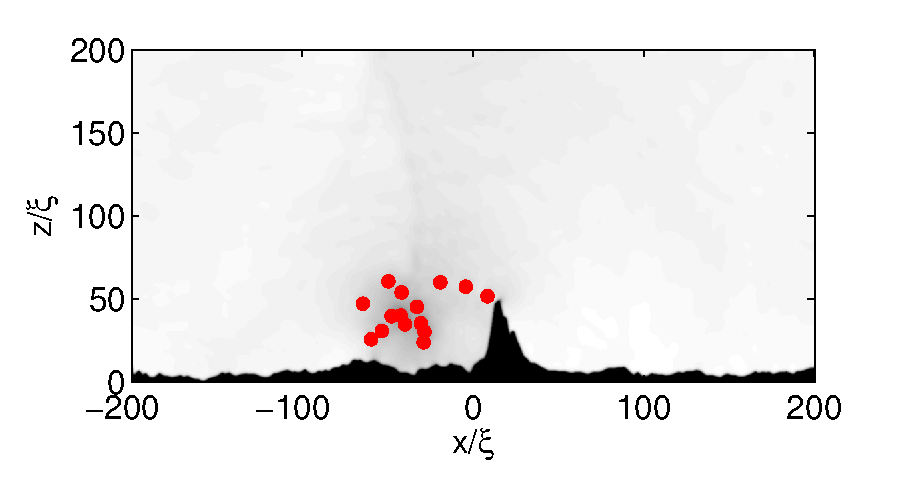
\includegraphics[width=0.35\linewidth]{./afm/figures/prog-35-500}\hspace{-0.6cm}
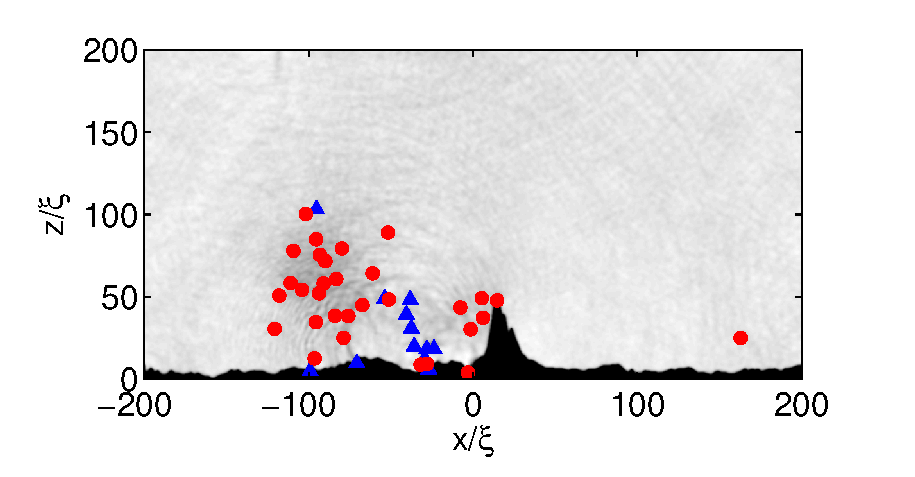
\includegraphics[width=0.35\linewidth]{./afm/figures/prog-35-1580}\hspace{-0.6cm}
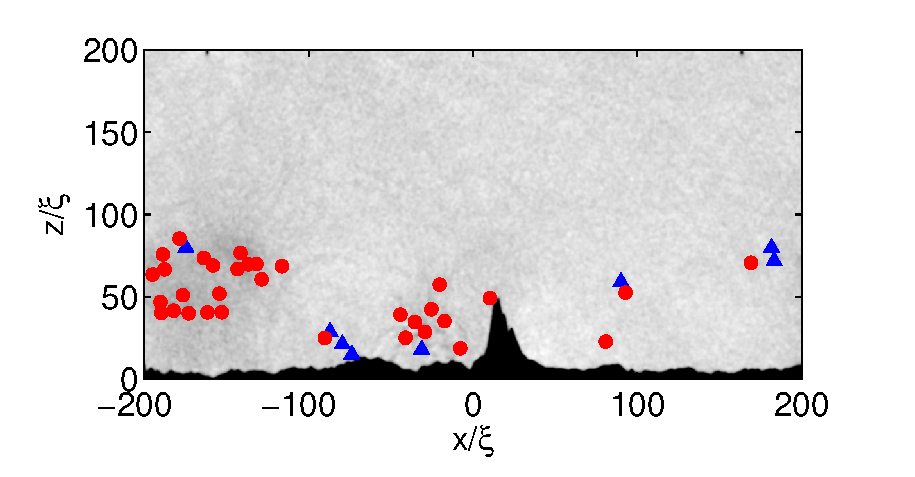
\includegraphics[width=0.35\linewidth]{./afm/figures/prog-35-2100}
\caption{\label{fig:prog} Evolution of 2D flow past the rough surface for a flow speed of $v=0.35c$.  Depicted are snapshots of density and vortex locations at times (from left to right) $t=500$, $1580$, and $2100~\tau$.  Red (blue) circles represent vortices of positive (negative) circulation.  }%Cluster forms, is interupped by secondary cluster and detaches. New cluster forms. }
\end{figure*}
\begin{figure*}
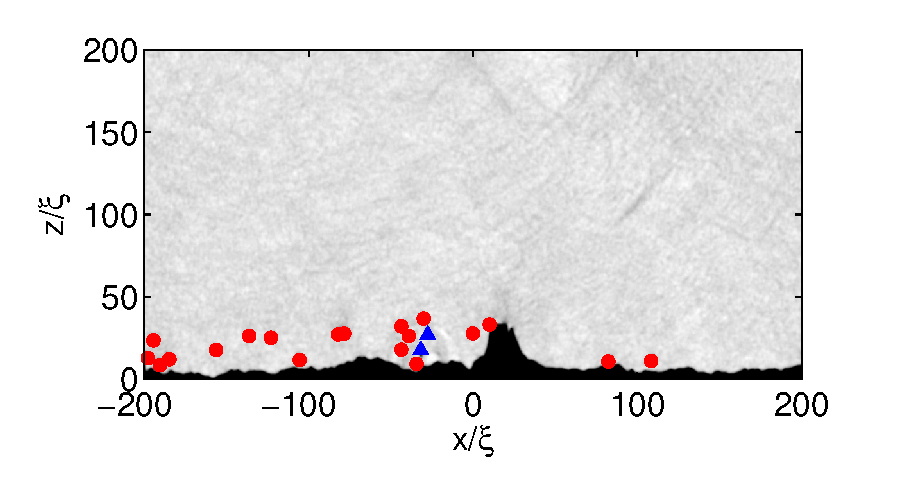
\includegraphics[width=0.35\linewidth]{./afm/figures/6th-35-2440}\hspace{-0.6cm}
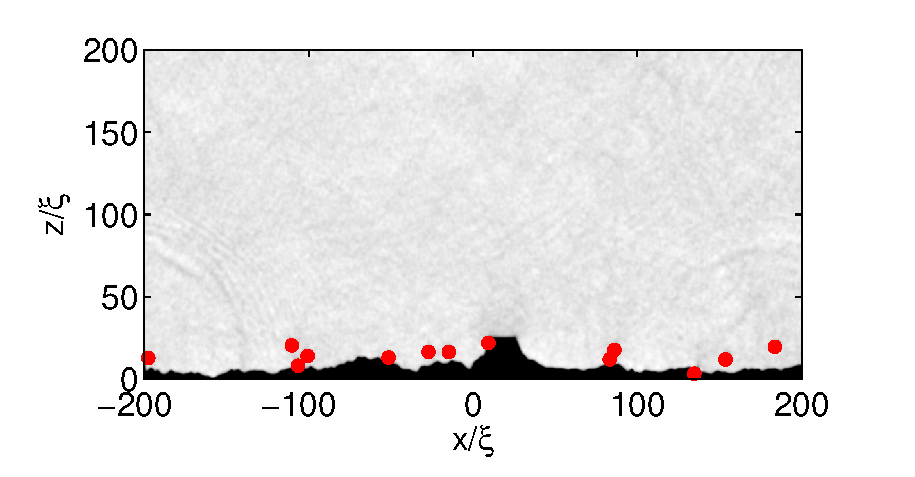
\includegraphics[width=0.35\linewidth]{./afm/figures/8th-35-2440}\hspace{-0.6cm}
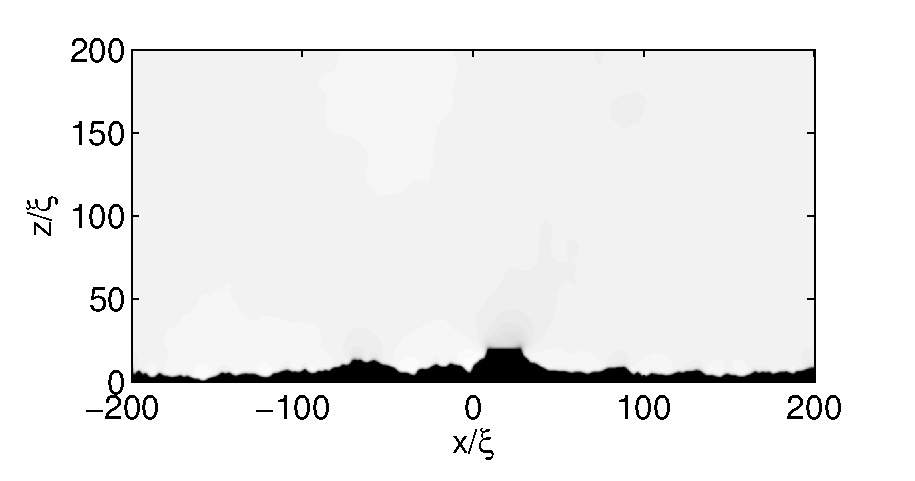
\includegraphics[width=0.35\linewidth]{./afm/figures/10th-35-2440}
\caption{\label{fig:trunc} Same-time snapshots for various levels of surface truncation: (i) $\beta=70\%$, (ii) $\beta=50\%$ and (iiii) $\beta=40\%$, where $\beta$ represents the truncation height relative to the highest point in the surface. Depicted are snapshots of density and vortex locations. For comparison, the untruncated surface ($\beta=100\%$) is depicted in Fig. \ref{fig:prog}.  The flow speed is $v=0.35c$ and the time is $t=2440\tau$.}
\end{figure*}
We find the critical velocity for vortex nucleation to be $v_c=(0.125\pm0.025) c$. We focus on an arbitrary super-critical flow speed of $v=0.35c$, with Fig. \ref{fig:prog} depicting the evolution of the system.  For clarity we show both the condensate density (upper plots) and vortex locations/circulation (lower plots).  At early times, a series of positive-circulation vortices (red) peel off from the peak of the large mountain. Vortices are nucleated here, and not elsewhere, due to the high curvature in the surface at this peak, which induces a relatively high local fluid velocity.  As they are carried downstream the vortices stay in close proximity and co-rotate about one another; this leads to the vortices combining into a larger-scale cluster of positive circulation.  This cluster travels downstream just above the surface.  Close to the surface, the cluster introduces a large relative fluid flow in the positive-$x$ direction.  This interrupts the nucleation of vortices from the mountain top and also induces the secondary generation of vortices (blue) from smaller-scale surface prominences.  These secondary vortices are of negative circulation and also form a vortex cluster. As this cluster grows, it leads to a cessation of secondary vortex production, and so again the primary vortices become nucleated from the mountain peak.  This process repeats.

The total number of vortices $N_v$ increases with time (Fig. \ref{fig:nvort}(a), solid line); initially this increase is rapid but over time it slows down as the number of vortices within the finite-sized box begins to saturate.  Initially this is almost entirely composed of positively-signed vortices (dashed line), apart from a small amount of spurious negative-sign vortices (dotted line).  At $t\approx 700 \tau$ the number of positive-sign vortices increases sharply; this represents the formation of secondary vortices. 

It is important to note that the generation of secondary clusters requires the surface to be rough downstream of the mountain.  If the surface is perfectly smooth downstream of the mountain, the positive-signed vortices persist.  

Note also that it is possible for tertiary vortices/clusters of positive-sign; these arise when the secondary cluster induces a sufficiently high flow speed in the negative-$x$ direction to generate vortices from the local surface roughness.

\subsection{Truncated surfaces}
It is evident above that the vortex generation is dominated by the large single prominence in the surface, with the smaller prominences having only a secondary effect.  To further analysis this we next study how the flow is affected by truncation of the surface height, $z=h(x,y)$, to a percentage $\beta$ of the maximum height $h_0$, i.e. $h(x,y) \rightarrow h(x,y) H(z/h_0=\beta)$, where $H(z)$ is the Heaviside step function ($\beta=100\%$ corresponds to no truncation, $\beta=0$ corresponds to complete truncation).

Figure \ref{fig:trunc} shows a snapshot (at fixed time) for various levels of truncation $\beta$, with all cases having the same flow speed $v=0.35c$.  It is evident that the height of the mountain plays a critical role.  Already, when the mountain is capped at $70\%$, the number of vortices produced by that time is vastly reduced.  The vortices are generated at a sufficiently low frequency that only small clusters form; secondary vortices are still formed but in a much lower quantity.  For $\beta=50\%$ even fewer vortices are produced, and for this case no clustering takes place and in turn no secondary vortices are formed.  For $\beta=40\%$ no vortices are generated at all.  

\begin{figure}
\centering
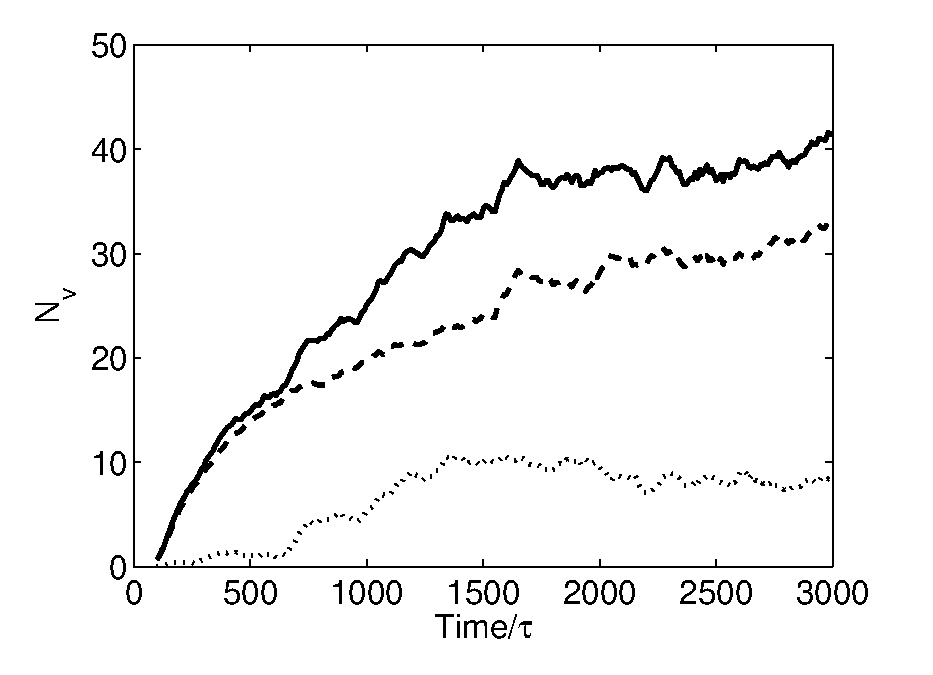
\includegraphics[width=0.45\linewidth]{./afm/figures/nvpn3bw}
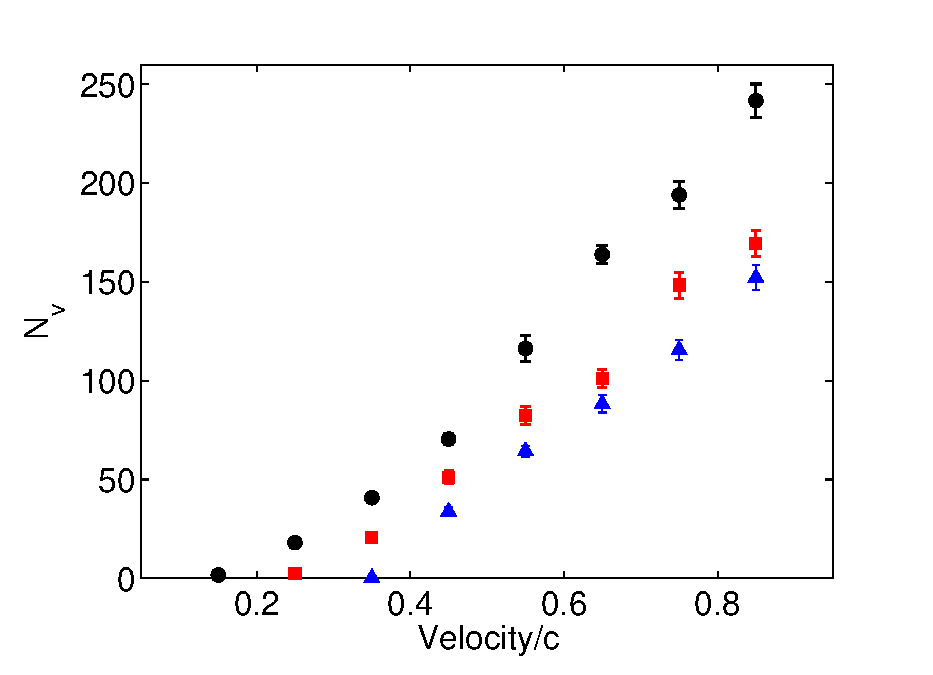
\includegraphics[width=0.45\linewidth]{./afm/figures/nv_v}
\caption{\label{fig:nvort} (a) Number of vortices produced during $v=0.35c$ flow past the surface.  Shown are the numbers of total vortices $N_v$ (solid line), positive vortices (dashed line) and negative vortices (dotted line). (b) Final number of vortices $N_v$ as a function of the flow velocity $v$ for the 2d simulations.  Each data point represents the average of 20 measurements of $N_v$ in the vicinity of $t=3000\tau$.}
\end{figure}  

\section{Conclusions}
In conclusion, our results suggest that the walls of channels which
confine the flow of superfluid liquid helium and the surfaces of moving
objects (wires, grids, propellers, spheres) which are used
to generate superfluid turbulence in current experiments
may be covered by a thin `superfluid boundary layer' consisting of 
vortex loops and rings.  This is a surprising effect, because
in fluid dynamics boundary layers usually arise from viscous forces, 
which in superfluid liquid helium near the temperature of
absolute zero are completely absent.  These findings further illustrate the deep analogies between classical and quantum fluids.
The experimental implications of `superfluid boundary layers` on macroscopic
observables need to be investigated.  Our results should
particularly stimulate experiments in $^3$He-B, where, due to relative
large healing length, it is possible to study flows with controlled 
surface height roughness. 

\end{chapter}

  \begin{chapter}{\label{cha:conc}Conclusions and future work}
\section{Conclusions}
In this chapter, we summarise the conclusions of the work presented throughout the thesis, and suggest relevant directions in which the work can be extended in the future. 

In Part I we introduced the mean-field theory that allows for accurate modelling of a dilute, weakly interacting Bose-Einstein condensate. We described the GPE, a non-linear Schr\"odinger equation used to model condensates at zero temperature, along with extensions to model finite temperatures through phenomenological damping and the classical-field method. We also described the theory and practice of various numerical procedures we have used throughout the thesis.

\subsubsection{Classical-like wakes behind elliptical obstacles in Bose-Einstein condensates}
In Chapter \ref{cha:wake} we showed that a 2D or 3D obstacle in the presence of superfluid flow in a Bose-Einstein condensate generates wakes of quantum vortices which resemble those of classical viscous flow past a cylinder or sphere.

We demonstrated a key ingredient to produce classical-like wakes: high vortex nucleation rate so that vortices undergo strong interactions with their neighbours, rather than being swept away. The role of ellipticity in this chapter was to reduce the critical velocity for vortex nucleation and increase vortex nucleation frequency and density, to facilitate strong interaction between vortices.  

The symmetric wakes produced are similar to those observed in classical flow at low $\Rey$. We showed that they are unstable, forming time-dependent asymmetric structures similar to the B\'enard--von K\'arm\'an vortex street of classical fluid dynamics.

The effects we described are relevant to the motion of objects such as vibrating wires, grids and forks in superfluid helium, where the obstacle's ellipticity plays a role which is analogous to rough boundaries \cite{blaz08,brad05}, and described patterns in the density distribution that could be potentially observed in experimental atomic Bose-Einstein condensates, with moving laser-induced potentials.

\subsubsection{Decay of 2D quantum turbulence in a highly oblate Bose-Einstein condensate}
In Chapter \ref{cha:shin} , we modelled the experimental set up of Kwon {\it et al.} in which the creation and decay of vortices within a BEC~\citep{kwon_moon_14} was observed. We showed that the system is well described by simulations of the 2D-GPE with phenomenological dissipation (despite the system's technically 3D nature). We elucidated the system's experimentally unobserved early stages, showing that vortex clusters form behind a laser-induced obstacle. We demonstrated that early time symmetry breaking causes disorganisation of the vortices and that by the time the obstacle is removed, the vortices are well randomised. We confirmed the occasional appearance of crescent-shaped density features, resulting either from the proximity of vortex cores or from a sound pulse which follows a vortex-antivortex reconnection.

We showed that the vortices decay in a manner which is consistent with the two mechanisms proposed by Kwon {\it et al.} (loss of vortices at the condensate edge due to thermal dissipation and vortex-antivortex annihilation events within the condensate) and fitted the rate equations proposed by Kwon {\it et al.} and Cidrim {\it et al.} to the vortex decay that we observed in our numerical simulations. We concluded that Cidrim's equation fits to the data most favourably, while providing physically realistic values for the decay rates.

\subsubsection{Quasi-classical turbulence and the critical velocity in a quenched Bose gas}
In Chapter \ref{cha:nonequib}, we modelled a finite temperature homogeneous Bose gas. We evolved the classical field from highly non-equilibrium initial conditions, through decay of a vortex tangle, to thermalised equilibrium states with a range of temperatures and condensate fractions.

We characterised the turbulent vortex tangle by finding a kinetic energy spectrum that demonstrates a {\it lack} of quasi-classical turbulence, and through tracking the vortex line-density over time, we found a decay rate characteristic of ultra-quantum turbulence. We confirmed the result by calculating the velocity correlation function and integral scale, finding them to be consistent with ultra-quantum turbulence.

With the resulting equilibrium states we inserted a cylindrical obstacle with Gaussian profile, and imposed a fluid flow.  We found that above the critical velocity, vortices are nucleated as wiggly vortex lines, vortex rings, or as a vortex tangle. We demonstrated that the critical velocity decreases with increasing temperature (becoming zero at the critical temperature for condensation) and scales with the square root of the condensate fraction.

\subsubsection{Simulating the rough surface of a ``Floppy Wire''}
In Chapter \ref{cha:afm}, we modelled the rough surface of a real ``floppy wire'' used in helium II experiments through a potential term in the zero temperature GPE and by imposing a flow. The surface of the wire was provided via atomic force microscopy. We performed two-dimensional simulations of the surface at various levels of truncation and at various flow speeds to probe the parameter space.

We observed for various truncations of the 2D profile and for several flow velocities in excess of the critical velocity, the formation of a `boundary layer' of quantum vortices. In each case, for a high enough imposed flow velocity the boundary layer effect breaks down and quantum vortices instead fill the computational box.

We performed large scale 3D simulations, showing that the boundary layer effect generalises to three dimensions. We showed evidence of a ``vortex mill'' mechanism leading to escaping vortex rings formed from the boundary layer. We measured the velocity profile of the fluid flow and demonstrated a qualitatively similar profile to those seen for boundary layers in classical viscous fluids.

Our results suggest that in superfluids the surfaces of moving objects may be covered by a thin `superfluid boundary layer' consisting of vortex loops and rings. This is a surprising effect: boundary layers usually arise from viscous forces, which in zero temperature superfluids are completely absent.

\section{Future work} 
\subsubsection{Other quantum analogues of classical-like wakes}
Many studies of viscous flow in classical fluids have been performed over the years. Collections such as Van Dyke's {\it Album of Fluid Motion} \cite{nagib} demonstrate the wide range of flows possible with various obstacle shapes and sizes in both 2D and 3D regimes. As an example, the wakes of rectangular (rather than circular) obstacles and recesses are shown in Figure \ref{fig:dyke-imgs}. Chapter \ref{cha:wake} investigated the classical-like wakes in the simplest case of a cylinder in quantum flow. It would be an extremely interesting direction for future work to attempt to experiment with the more complicated examples of classical flow patterns that exist in the literature. The idea that the behaviour of many quantum vortices collectively reproduces classical physics would suggest that perhaps other analogies of classical fluid wakes exist in the quantum fluid realm. 
\begin{figure}
\centering
    \includegraphics[width=\linewidth]{wake/square.png}
  \caption{Various examples of classical viscous fluid flow around square obstacles and recesses \cite{nagib}.} 
  \label{fig:dyke-imgs}
\end{figure}

\subsubsection{Finite temperature trapped Bose gas}
While the work set our in Chapter \ref{cha:nonequib} is based on a homogeneous system, in reality Bose-Einstein condensates are experimentally confined in traps, rendering the gas inhomogeneous. One can expect significant corrections to the critical velocity due to density gradients, as well as modifications to the vortex nucleation pattern. It would be interesting to see these higher order effects studied in future works, in particular in the common case of a harmonic trapping potential.

On the other hand, recent advances have led to the formation of quasi-homogeneous condensates in box-like traps \cite{gaunt_2013,chomaz_2015}. Here, the higher order corrections associated with trapping inhomogeneity should have minimal effect. An interesting direction for future experimental work would be to compare our experimentally measurable numerical predictions, such as critical velocity or the vortex line-density decay rate, to experimental data incorporating quasi-homogeneous box-like traps.

\subsubsection{Exploring the superfluid boundary layer}
The experimental implications of possible `superfluid boundary layers`, demonstrated in Chapter \ref{cha:afm}, on macroscopic observables need to be investigated.  The results we have shown in 3D should particularly stimulate experiments in $^3$He-B, where, due to relative
large healing length, it is possible to observe vortex core structure and study flows with controlled surface height roughness.

An alternative experimental application of the 2D boundary layers observed in Chapter \ref{cha:afm} can be found in the context of atomic BECs. Recently, the path has opened towards the realisation of dynamic and arbitrarily shaped obstacles \cite{Henderson09}. By utilizing arbitrary potentials, a moving rough surface could be implemented in a quasi-two-dimensional atomic BEC.

Numerically there is also much work to still be done, particularly in 3D. While current computational limits are reached quickly with our simulations, the potential future increase in power of high performance clusters or even desktop computers could allow for quicker numerical simulation and easier visualisation of results. Along these lines, a potential extension to the work in Chapter \ref{cha:afm} is the undertaking of a significant exploration of the 3D parameter space. It would be interesting to explore the response to changes to the imposed superfluid flow speed and surface roughness through truncation, and if the behaviour generalises from our two-dimensional results to the three-dimensional case.
\end{chapter}

  \part{Appendix}
  \appendix
  \begin{chapter}{
\label{app:App1}My appendix title}
\end{chapter}
\begin{chapter}{
\label{app:App2}Calculating various properties}
\section{\label{appsection:energy} Energy}
\section{\label{appsection:force} Force}
\end{chapter}                    % An appendix.

  % Uncomment the line below if you want your Bibliography to appear in the
  % table of contents.
  \addcontentsline{toc}{chapter}{Bibliography}
  \bibliography{references}             % References.
  \bibliographystyle{apsrev}
%  \printindex
\end{document}
